\pdfoutput=1
\documentclass[journal, 10pt]{IEEEtran}
\IEEEoverridecommandlockouts
%\documentclass[11pt,draftcls,onecolumn]{IEEEtran}
%\usepackage{geometry}   
%\usepackage[margin=1in]{geometry}             % See geometry.pdf to learn the layout options. There are lots.
%\geometry{letterpaper}                   % ... or a4paper or a5paper or ... 
%\geometry{landscape}                % Activate for for rotated page geometry
%\usepackage[parfill]{parskip}    % Activate to begin paragraphs with an empty line rather than an indent
\usepackage{graphicx}
\usepackage{amssymb}
\usepackage{amsmath}
\usepackage{amsthm}
\usepackage{amsfonts}
\usepackage{hyperref,algorithm}
\usepackage{algpseudocode}
\usepackage{mathtools}
\usepackage{epstopdf}
\usepackage{dblfloatfix}
\usepackage{color}
\usepackage{array}
\usepackage{arydshln}
\usepackage{multirow}
\usepackage{booktabs}
\usepackage{balance}
\usepackage{setspace}
\DeclareGraphicsRule{.tif}{png}{.png}{`convert #1 `dirname #1`/`basename #1 .tif`.png}
\newtheorem{theorem}{\textbf{Theorem}}
\newtheorem{definition}{\textbf{Definition}}
\newtheorem{problem}{\textbf{Problem}}
\newtheorem{example}{\textbf{Example}}
\newtheorem{remark}{\textbf{Remark}}
\newtheorem{lemma}{\textbf{Lemma}}
\newtheorem{corollary}{\textbf{Corollary}}
\newtheorem{proposition}{\textbf{Proposition}}
\newcommand{\transpose}{{\!\scriptscriptstyle\mathrm T}}
\newcommand{\norm}[1]{\lVert#1\rVert}
\newcommand{\R}{\mathbb{R}}
\renewcommand{\l}{\ell}
\newcommand{\Identity}{1\!\!1}
\newcommand{\G}{{\mathcal{G}}}
\newcommand{\E}{{\mathcal{E}}}
\newcommand{\W}{{\mathcal{W}}}
\newcommand{\V}{{\mathcal{V}}}
\newcommand\ip[2]{\langle #1, #2\rangle}
\usepackage{array}
\newcolumntype{L}[1]{>{\raggedright\let\newline\\\arraybackslash\hspace{0pt}}m{#1}}
\newcolumntype{C}[1]{>{\centering\let\newline\\\arraybackslash\hspace{0pt}}m{#1}}
\newcolumntype{R}[1]{>{\raggedleft\let\newline\\\arraybackslash\hspace{0pt}}m{#1}}
\renewcommand{\L}{\boldsymbol{\mathcal{L}}}
 \DeclareMathOperator*{\argmax}{argmax}
 \DeclareMathOperator*{\argmin}{argmin}
\newcommand{\Expectation}{I\!\!E} %expectation
\renewcommand{\IEEEbibitemsep}{0pt plus 0.5pt}
\newcommand{\change}[1]{{\color{blue} {#1} }}
\makeatletter
\IEEEtriggercmd{\reset@font\normalfont\fontsize{7.5pt}{8.0pt}\selectfont}
\makeatother
\IEEEtriggeratref{1}


\begin{document}

\title{
A Scalable $M$-Channel Critically Sampled Filter Bank for Graph Signals 
}
\author{\IEEEauthorblockN{Yan Jin, Shuni Li, and David I Shuman}
%\thanks{Copyright (c) 2015 IEEE. Personal use of this material is permitted. However, permission to use this material for any other purposes must be obtained from the IEEE by sending a request to pubs-permissions@ieee.org.}
\thanks{Yan Jin is with the Institute for Data, Systems, and Society, Massachusetts Institute of Technology, Cambridge, MA 02139, USA (email: yjin1@mit.edu). Shuni Li and David I Shuman are with the Department of Mathematics, Statistics, and Computer Science, Macalester College, St. Paul, MN 55105, USA (email: \{sli,dshuman1\}@macalester.edu).  }
\thanks{This research has been funded in part by a grant to Macalester College from the Howard Hughes Medical Institute through the Precollege and Undergraduate Science Education Program.}
\thanks{The authors would like to thank Federico Poloni for providing a proof to Proposition \ref{Pr:mat_part}, and Andrew Bernoff for helpful discussions about the matrix partitioning problem discussed in Section \ref{Se:partition}.}
\thanks{MATLAB code for all numerical experiments in this paper is available at \url{http://www.macalester.edu/\textasciitilde dshuman1/publications.html}. It leverages the open access GSPBox \cite{gspbox}, into which it will soon be integrated.}}

\maketitle

%\begin{abstract}
%We investigate an $M$-channel critically sampled filter bank for graph signals where each of the $M$ filters is supported on a different subband of the graph Laplacian spectrum. We partition the graph vertices such that the $m^{th}$ set comprises a uniqueness set for signals supported on the $m^{th}$ subband. For analysis, the graph signal is filtered on each subband and downsampled on the corresponding set of vertices. However, the classical synthesis filters are replaced with interpolation operators, circumventing the issue of how to design a downsampling pattern and graph spectral filters to ensure perfect reconstruction for signals that do not reside on bipartite graphs. The resulting transform is critically sampled and graph signals are perfectly reconstructable from their analysis coefficients. We empirically explore the joint vertex-frequency localization of the dictionary atoms and sparsity of the analysis coefficients, as well as the ability of the proposed transform to compress 
%piecewise-smooth graph signals. {\color{red} Update abstract.}
%\end{abstract}

\begin{abstract}
We investigate a scalable $M$-channel critically sampled filter bank for graph signals, where each of the $M$ filters is supported on a different subband of the graph Laplacian spectrum. For analysis, the graph signal is filtered on each subband and downsampled on a corresponding set of vertices. However, the classical synthesis filters are replaced with interpolation operators. For small graphs, we use a full eigendecomposition of the graph Laplacian to partition the graph vertices such that the $m^{th}$ set comprises a uniqueness set for signals supported on the $m^{th}$ subband. The resulting transform is critically sampled, the dictionary atoms are orthogonal to those supported on different bands, and graph signals are perfectly reconstructable from their analysis coefficients. We also investigate a fast version of the proposed transform that scales efficiently for large, sparse graphs. Issues that arise in this context include designing the filter bank to be more amenable to polynomial approximation, estimating the number of samples required for each band, performing non-uniform random sampling for the filtered signals on each band, and efficient reconstruction methods. We empirically explore the joint vertex-frequency localization of the dictionary atoms, the sparsity of the analysis coefficients for different classes of signals, the ability of the proposed transform to compress piecewise-smooth graph signals, and the reconstruction error resulting from the numerical approximations.
\end{abstract}

\begin{IEEEkeywords}
Graph signal processing, filter bank, non-uniform random sampling, interpolation, wavelet, compression
\end{IEEEkeywords}
%

\section{Introduction}

In graph signal processing \cite{shuman2013emerging}, transforms and filter banks can help exploit structure in the data, in order, for example, to compress a graph signal, remove noise, or fill in missing information. 
Broad classes of recently proposed transforms include graph Fourier transforms, vertex domain designs such as \cite{Crovella2003,wang}, top-down approaches such as \cite{szlam,gavish,irion}, diffusion-based designs such as \cite{coifman2006diffusion,Maggioni_biorthogonal}, spectral domain designs such as \cite{hammond2011wavelets,shuman2013spectrum}, windowed graph Fourier transforms  \cite{shuman2015vertex}, and generalized filter banks, the last of which we focus on in this paper. For further introduction to dictionary designs for graph signals, see \cite{shuman2013emerging}.


\begin{figure}[t]
\centerline{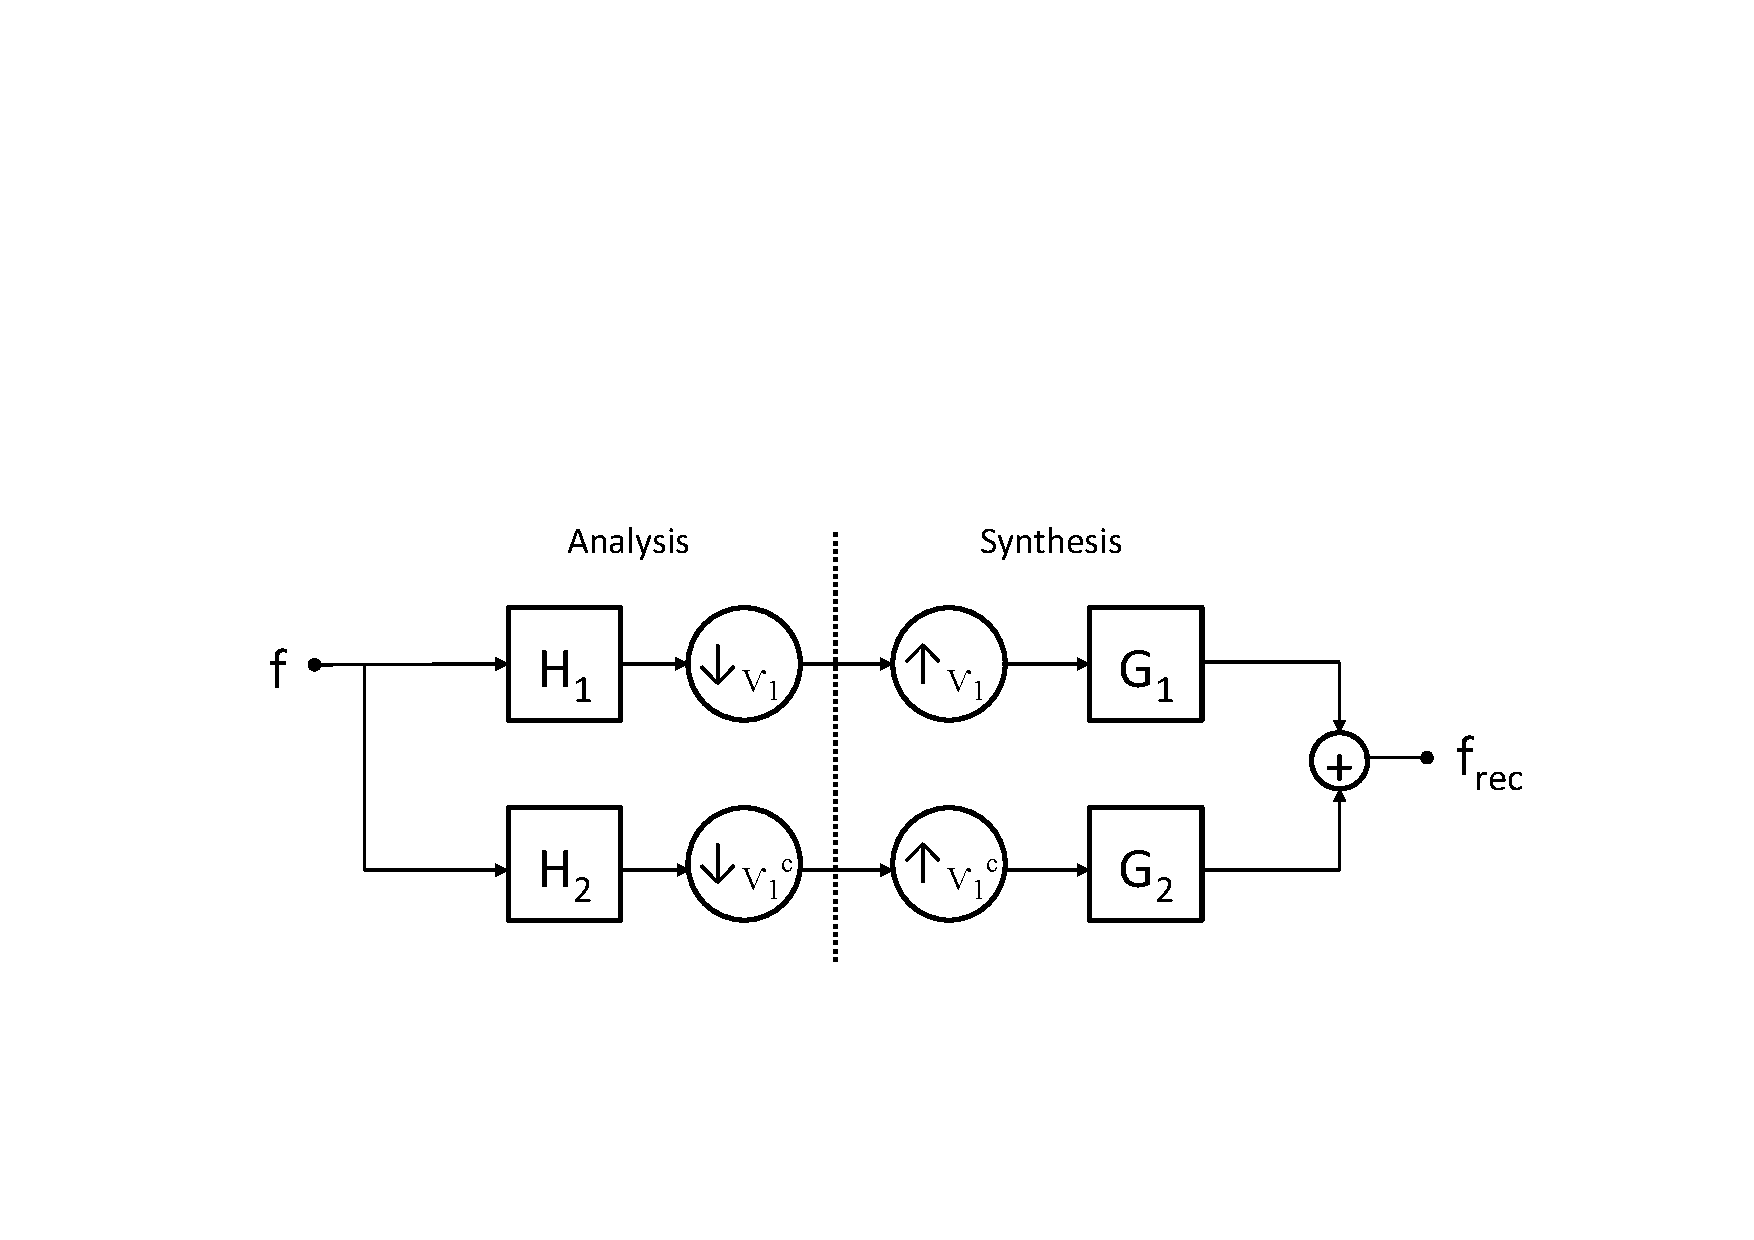
\includegraphics[width=3.3in]{fig_two_channel_classical}}
\caption{Extension of the classical two channel critically sampled filter bank to the graph setting. Here, $\mathbf{H}_1$ is a lowpass graph spectral filter, and $\mathbf{H}_2$ is a highpass graph spectral filter.}\label{Fig:two_channel}
\end{figure}


The extension of the classical two channel critically sampled filter bank to the graph setting was first proposed in \cite{narang_icip}. Fig.\ \ref{Fig:two_channel} shows the analysis and synthesis banks, where ${\bf H}_i$ and ${\bf G}_i$ are graph spectral filters \cite{shuman2013emerging}, and the lowpass and highpass bands are downsampled on complementary sets of vertices. For a general weighted, undirected graph, it is not straightforward %{\color{red} (impossible?)} 
how to design the downsampling and the four graph spectral filters to ensure perfect reconstruction. One approach is to separate the graph into a union of subgraphs, each of which has some regular structure. For example, \cite{narang2012perfect,narang_bior_filters} show that the normalized graph Laplacian eigenvectors of \emph{bipartite} graphs have a spectral folding property that make it possible to design analysis and synthesis filters to guarantee perfect reconstruction. They take advantage of this property by decomposing the graph into bipartite graphs and constructing a multichannel, separable filter bank, while \cite{sakiyama} adds vertices and edges to the original graph to form an approximating bipartite graph. References \cite{teke2016,teke2017ii} generalize this spectral folding property to $M$-block cyclic graphs, and leverage it to construct $M$-channel graph filter banks. Another class of regular structured graphs is \emph{shift invariant} graphs \cite[Chapter 5.1]{grady}. These graphs have a circulant graph Laplacian and their eigenvectors are the columns of the discrete Fourier transform matrix. Any graph can be written as the sum of circulant graphs, and \cite{ekambaram_icip,ekambaram2013globalsip,kotzagiannidis2016icassp} take advantage of this fact in designing critically sampled graph filter banks with perfect reconstruction. Another approach is to use architectures other than the critically sampled filter bank, such as lifting transforms \cite{jansen,narang_lifting_graphs} or pyramid transforms \cite{shuman_TSP_multiscale}.

Our approach in this paper is to replace the synthesis filters with interpolation operators on each subband of the graph spectrum. While this idea was initially suggested independently in \cite{chen2015discrete}, we investigate it in more detail here. Our construction leverages the recent flurry of work in sampling and reconstruction of graph signals \cite{chen2015discrete}-\nocite{pesenson_paley,narang2013interpolation,anis2014towards,gadde2015probabilistic,shomorony,PuyTGV15,chen2015signal,tsitsvero2016uncertainty,chen2016signal}\cite{anis2016efficient}. The key property we use is that any signal whose graph Fourier transform has exactly $k$ non-zero coefficients can be perfectly recovered from samples of that signal on $k$ appropriately selected vertices (see, e.g., \cite[Theorem 1]{chen2015discrete} \cite[Proposition 1]{anis2016efficient}).

{\color{red} Add to intro here: scalable issues, outline, and contribution relative to conference paper.}


\section{$M$-Channel Critically Sampled Filter Bank}
We consider graph signals $f \in \R^N$ residing on a weighted, undirected graph $\G=\{\V,\E,\mathbf{W}\}$, where $\V$ is the set of $N$ vertices, $\E$ is the set of edges, and $\mathbf{W}$ is the weighted adjacency matrix. 
Throughout, we take $\L$ to be the combinatorial graph Laplacian $\mathbf{D}-\mathbf{W}$, where $\mathbf{D}$ is the diagonal matrix of vertex degrees. However, our theory and proposed transform also apply to the normalized graph Laplacian $\mathbf{I}-\mathbf{D}^{-\frac{1}{2}}\mathbf{W}\mathbf{D}^{-\frac{1}{2}}$, or any other Hermitian operator. We can diagonalize the graph Laplacian as $\L=\mathbf{U}{\boldsymbol \Lambda}\mathbf{U}^{*}$, where ${\boldsymbol \Lambda}$ is the diagonal matrix of eigenvalues $\lambda_0,\lambda_1,\ldots,\lambda_{N-1}$ of $\L$, and the columns ${\bf u}_0,{\bf u}_1,\ldots,{\bf u}_{N-1}$ of $\mathbf{U}$ are the associated eigenvectors of $\L$. The graph Fourier transform of a signal is $\hat{\bf{f}}=\mathbf{U}^{*}{\bf f}$, and ${h}(\L){\bf f}=\mathbf{U}{h}({\boldsymbol \Lambda})\mathbf{U}^{*}{\bf f}$ applies the filter ${h}: [0,\lambda_{\max}] \rightarrow \R$ to the graph signal ${\bf f}$. We use the notation $\mathbf{U}_{{\cal R}}$ to denote the submatrix formed by taking the columns of $\mathbf{U}$ associated with the Laplacian eigenvalues indexed by ${\cal R} \subseteq \{0,1,\ldots,N-1\}$. Similarly, we use the notation $\mathbf{U}_{{\cal S},{\cal R}}$ to denote the submatrix  formed by taking the rows of $\mathbf{U}_{{\cal R}}$ associated with the vertices indexed by the set ${\cal S} \subseteq \{1,2,\ldots,N\}$.

We start by constructing an ideal filter bank of $M$ graph spectral filters, where for a set of band endpoints $0=\tau_0 < \tau_1 < \ldots < \tau_{M-1} \leq \tau_M$ (with $\tau_M > \lambda_{\max}$), the $m^{th}$ filter is defined as
\begin{align} \label{Eq:bandpass}
{h}_m(\lambda)=
\begin{cases}
1,& \tau_{m-1} \leq \lambda < \tau_m  \\
0,&\hbox{ otherwise}
\end{cases},~m=1,2,\ldots,M.
\end{align}
%\{\tau_m\}each filter ${h}_m(\lambda)$ is equal to 1 on a subset of the spectrum, and 0 elsewhere.
%We choose the filters so that for each $\l \in \{0,1,\ldots,N-1\}$, ${h}_m(\lambda_\l)=1$ for exactly one $m$. 
 Fig. \ref{Fig:fb} shows an example of such an ideal filter bank. Note that for each $\l \in \{0,1,\ldots,N-1\}$, ${h}_m(\lambda_\l)=1$ for exactly one $m$. 
Equivalently, we are forming a partition $\{{\cal R}_1,{\cal R}_2,\ldots,{\cal R}_M\}$ of $\{0,1,\ldots,N-1\}$ and setting
\begin{align*}
{h}_m(\lambda_{\l})=
\begin{cases}
1,&\hbox{ if } {\l} \in {\cal R}_m \\
0,&\hbox{ otherwise}
\end{cases},~m=1,2,\ldots,M.
\end{align*}

\begin{figure}[t]
\centerline{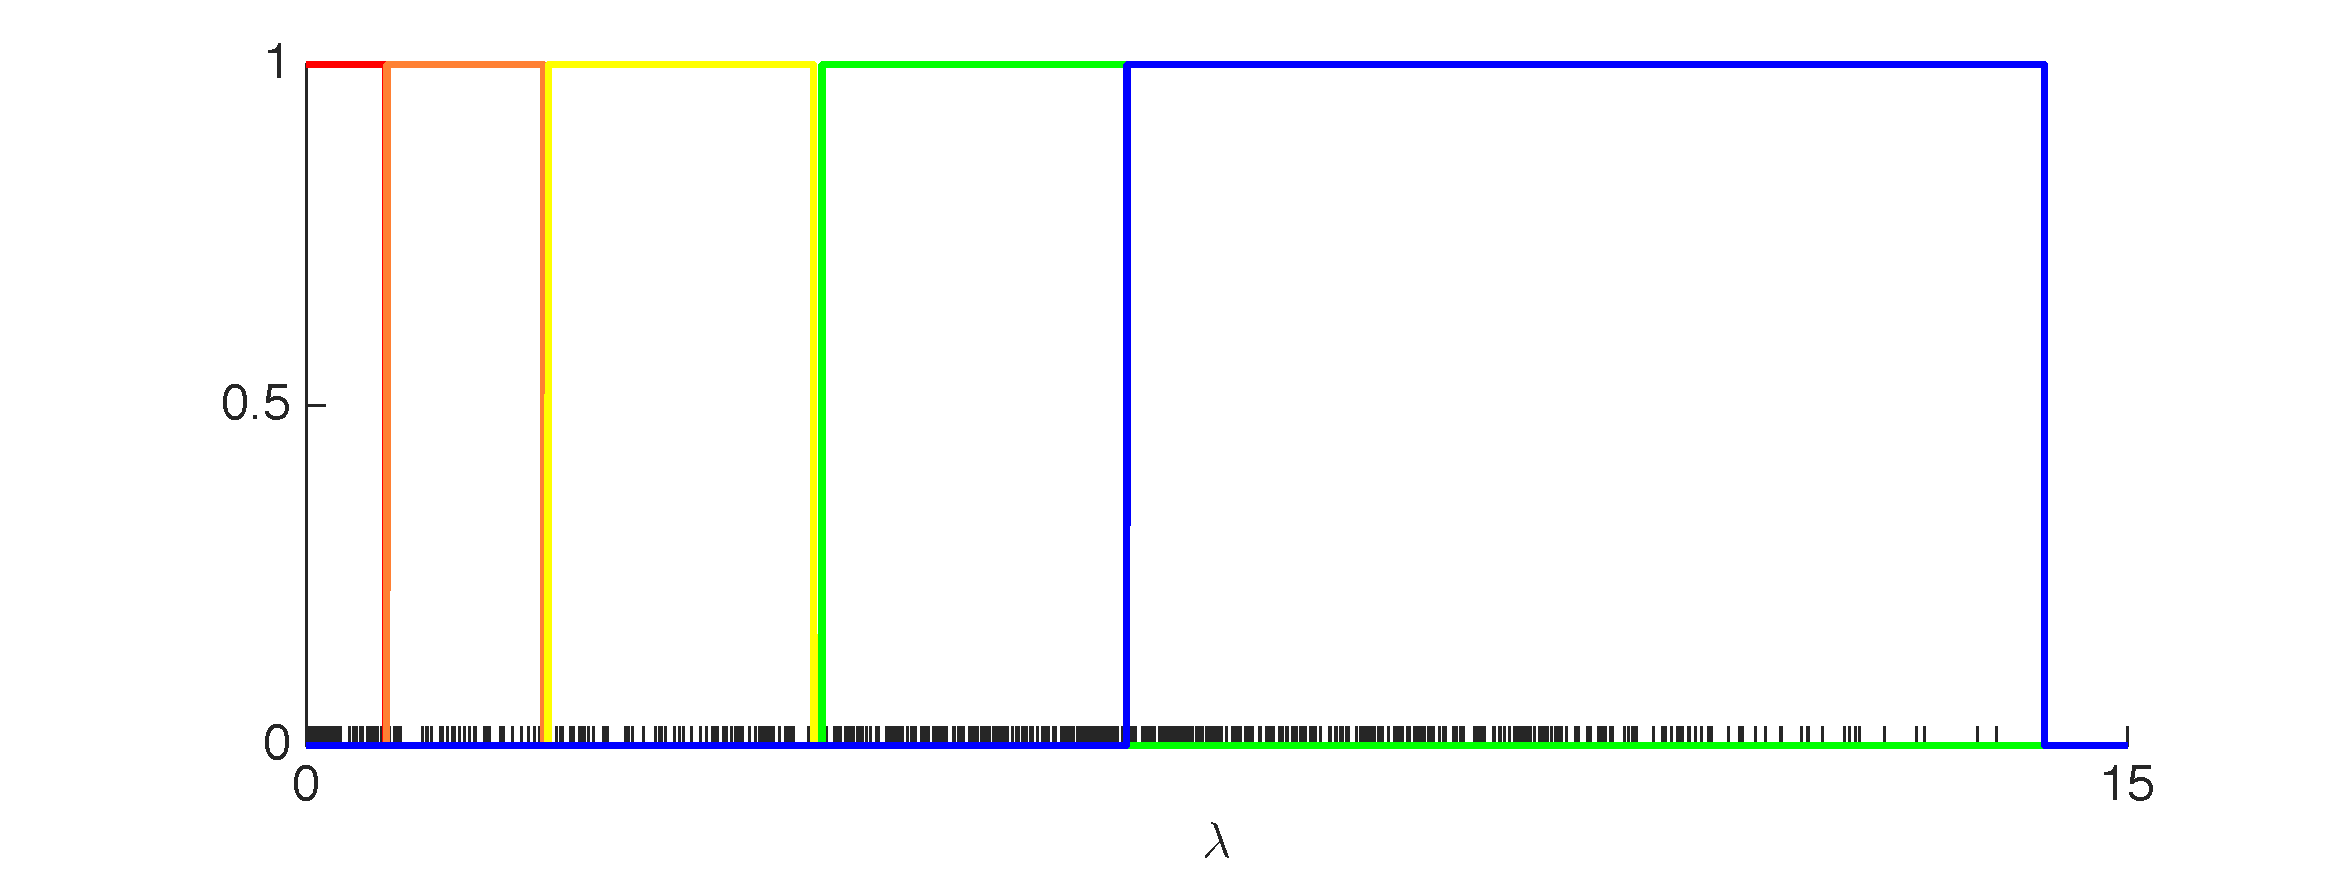
\includegraphics[width=3.1in]{fig_filter_bank}}
\caption{Example ideal filter bank. The red, orange, yellow, green, and blue filters span 31, 31, 63, 125, and 250 graph Laplacian eigenvalues, respectively, on a 500 node sensor network with %500 vertices and 
a maximum graph Laplacian eigenvalue of 14.3. The tick marks on the x-axis represent the locations of the graph Laplacian eigenvalues.}\label{Fig:fb}
\end{figure}

The next step, which we discuss in detail in the next section, is to partition the vertex set $\V$ into subsets $\V_1,\V_2,\ldots,\V_M$ such that $\V_m$ forms a uniqueness set for $\mbox{col}\left(\mathbf{U}_{{\cal R}_m}\right)$.
%the subband ${\cal R}_m$. 
\begin{definition}[Uniqueness set \cite{pesenson_paley}] 
%Let $${\cal R}=\{r_1,r_2,\ldots,r_K\} \subseteq \{0,1,\ldots,N-1\}$$ be a subset of the graph Laplacian eigenvalue indices. 
Let ${\cal P}$ be a subspace of $\R^n$. 
Then a subset $\V_s$ of the vertices $\V$ is a uniqueness set for 
%the subspace $\mbox{col}\left({\mathbf{U}}_{{\cal R}}\right)=\mbox{span}\{u_{r_1},u_{r_2}\ldots,u_{r_K}\} \subseteq \R^n$ 
${\cal P}$ if  and only if for all %$f,g \in \mbox{col}\left({\mathbf{U}}_{{\cal R}}\right)$, 
${\bf f},{\bf g} \in {\cal P}$,
${\bf f}_{\V_s}={\bf g}_{\V_s}$ implies ${\bf f}={\bf g}$. That is, if two signals in ${\cal P}$ have the same values on the vertices in the uniqueness set $\V_s$, then they must be the same signal.
\end{definition}
The following equivalent characterization of a uniqueness set is often useful.
\begin{lemma}[\cite{anis2014towards}, \cite{shomorony}]\label{Le:eq_uniq}
The set $\mathcal{S}$ of $k$ vertices is a uniqueness set for $\mbox{col}({\mathbf{U}}_{\mathcal T})$ if and only if the matrix whose columns are ${\bf u}_{{\mathcal T}_1},{\bf u}_{{\mathcal T}_2},\ldots,{\bf u}_{{\mathcal T}_k}, {\boldsymbol \delta}_{{\mathcal{S}}^c_1}, {\boldsymbol \delta}_{{\mathcal{S}}^c_2}, \ldots, {\boldsymbol \delta}_{{\mathcal{S}}^c_{n-k}}$ is nonsingular,
where each ${\boldsymbol \delta}_{{\mathcal{S}}^c_i}$ is a Kronecker delta centered on a vertex not included in $S$. 
\end{lemma}
The $m^{th}$ channel of the analysis %filter 
bank %then 
filters the graph signal by an ideal %low pass 
filter on subband ${\cal R}_m$, and downsamples the result onto the vertices in $\V_m$. For synthesis, we can interpolate from the samples on $\V_m$ to $\mbox{col}\left(\mathbf{U}_{{\cal R}_m}\right)$. Namely, denoting the analysis coefficients of the $m^{th}$ branch by ${\bf y}_{\V_m}$, we have
\begin{align} \label{Eq:synth}
{\bf f}_{rec} = \sum_{m=1}^M  \mathbf{U}_{{\cal R}_m} \mathbf{U}_{\V_m,{\cal R}_m}^{-1} {\bf y}_{\V_m}.
\end{align}
% the standard least squares reconstruction is to solve $x_m^*=\argmin_{x \in \R^{k_m}} ||\mathbf{U}_{{\cal R}_m}x - y_{\V_m} ||_2$, and let $f_{m,{rec}}(\V_m)=y_{\V_m}$ and $f_{m,{rec}}(\V_m^c)=\mathbf{U}_{\V_m^c,{\cal R}_m}x_m^*$; 
If there is no error in the coefficients, then the reconstruction is perfect, because $\V_m$ is a uniqueness set for $\mbox{col}\left(\mathbf{U}_{{\cal R}_m}\right)$, ensuring $\mathbf{U}_{\V_m,{\cal R}_m}$ is full rank. Fig.\ \ref{Fig:arch} shows the architecture of the proposed $M$-channel critically sampled filter bank (M-CSFB) with interpolation on the synthesis side.

\begin{figure}[t]
\centerline{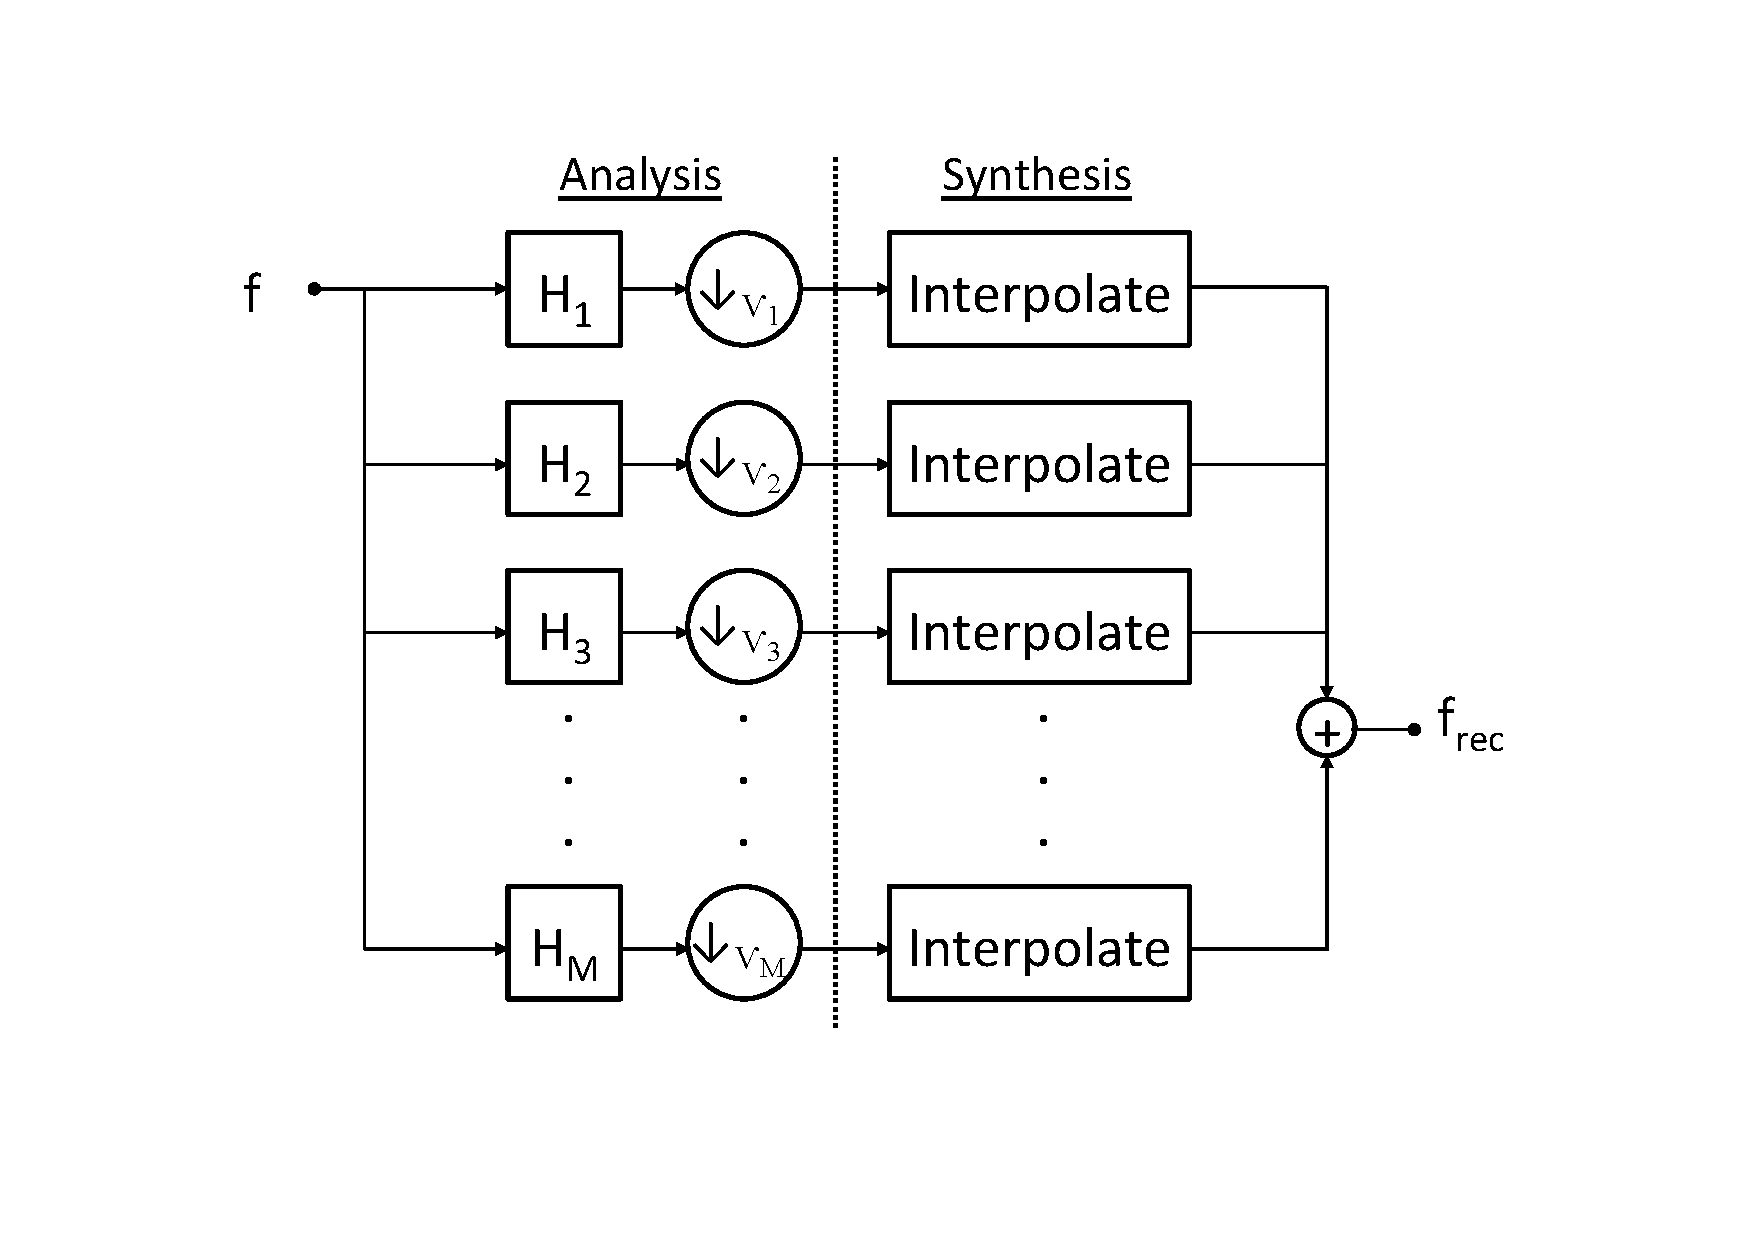
\includegraphics[width=2.8in]{fig_mcsfb_structure3}}
\caption{The $M$-channel critically sampled filter bank architecture. The sets $\V_1, \V_2, \ldots,\V_M$ form a partition of the set $\V$ of vertices, where each set $\V_m$ is a uniqueness set for graph signals supported on a different subband in the graph spectral domain.}\label{Fig:arch}
\end{figure}




\section{Partitioning the Graph into Uniqueness Sets for Different Frequency Bands}\label{Se:partition}

In this section, we show how to partition the set of vertices into uniqueness sets for different subbands of the graph Laplacian eigenvectors. We start with the easier case of $M=2$ and then examine the general case.

\subsection{$M=2$ channels}
%easier result that i
First we show that if a set of vertices is a uniqueness set for a set of signals contained in a band of spectral frequencies, then the complement set of vertices is a uniqueness set for the set of signals with no energy in that band of spectral frequencies.
\begin{proposition}\label{Le:highpass_uniqueness}
On a graph ${\mathcal G}$ with $N$ vertices, let 
${\mathcal T} \subseteq \{0,1,\ldots,N-1\}$ denote a subset of the graph Laplacian eigenvalue indices, and let ${\mathcal T}^c=\{0,1,\ldots,N-1\} \setminus {\mathcal T}$.
Then 
$\mathcal{S}^c$ is a uniqueness set for $\mbox{col}({\mathbf{U}}_{{\mathcal T}^c})$
 if and only if
$\mathcal{S}$ is a uniqueness set for 
$\mbox{col}({\mathbf{U}}_{{\mathcal T}})$.
\end{proposition}
This fact follows from either the CS decomposition \cite[Equation (32)]{paige})
%of C.C. Paige and M. Wei, "History and generality of the CS decomposition," Linear Algebra and Its Applications, 1992), 
or the nullity theorem \cite[Theorem 2.1]{strangInterplay}.  
%of G. Strang and T. Nguyen, "The interplay of ranks and submatrices," SIAM Review, 2004). 
We also provide a standalone proof below that only requires that the space spanned by the first $k$ columns of ${\mathbf{U}}$ is orthogonal to the space spanned by the last $N-k$ columns, not that ${\mathbf{U}}$ is an orthogonal matrix.

\begin{proof}[Proof of Proposition \ref{Le:highpass_uniqueness}]
We assume without loss of generality that ${\mathcal T}=\{0,1,2,\ldots,k-1\}$. 
Suppose first that the set $\mathcal{S}$ is a uniqueness set for $\mbox{col}({\mathbf{U}}_{\mathcal T})$, but $\mathcal{S}^c$ is not a uniqueness set for $\mbox{col}({\mathbf{U}}_{{\mathcal T}^c})$. Then by Lemma \ref{Le:eq_uniq}, the matrix $$\mathbf{A}=
 \left[ \begin{array}{cccccccc}
{\bf u}_{0} & {\bf u}_{1} & \cdots & {\bf u}_{k-1} & {\boldsymbol \delta}_{{\mathcal{S}}^c_1} & {\boldsymbol \delta}_{{\mathcal{S}}^c_2} \cdots & {\boldsymbol \delta}_{{\mathcal{S}}^c_{N-k}} \end{array} \right]$$
has full rank, and the matrix $$\mathbf{B}=
 \left[ \begin{array}{cccccccc}
{\bf u}_{k} & {\bf u}_{k+1} & \cdots & {\bf u}_{N-1} & {\boldsymbol \delta}_{\mathcal{S}_{1}} & {\boldsymbol \delta}_{\mathcal{S}_{2}} \cdots & {\boldsymbol \delta}_{\mathcal{S}_k} \end{array} \right]$$
is singular, implying
\begin{align}\label{Eq:span}
\mbox{span}({\bf u}_{k}, {\bf u}_{k+1},\ldots, {\bf u}_{N-1}, {\boldsymbol \delta}_{\mathcal{S}_{1}}, {\boldsymbol \delta}_{\mathcal{S}_{2}}, \ldots, {\boldsymbol \delta}_{\mathcal{S}_k}) \neq \mathbb{R}^N.
\end{align}
Since 
$$\mbox{dim}(\mbox{span}({\bf u}_{k}, {\bf u}_{k+1},\ldots, {\bf u}_{N-1}))=N-k$$ and $$\mbox{dim}(\mbox{span}({\boldsymbol \delta}_{S_{1}}, {\boldsymbol \delta}_{S_{2}}, \ldots, {\boldsymbol \delta}_{\mathcal{S}_k}))=k,$$ equation 
\eqref{Eq:span} implies that
there must exist a vector ${\bf x} \neq {\bf 0}$ such that 
\begin{align*}
&{\bf x} \in  \mbox{span}({\bf u}_{k}, {\bf u}_{k+1},\ldots, {\bf u}_{N-1})  \hbox{ and } \\
& {\bf x} \in \mbox{span}({\boldsymbol \delta}_{\mathcal{S}_{1}}, {\boldsymbol \delta}_{\mathcal{S}_{2}}, \ldots, {\boldsymbol \delta}_{\mathcal{S}_{k}}).\end{align*}
Yet, ${\bf x} \in \mbox{col}({\mathbf{U}}_{{\mathcal T}^c})$ implies ${\bf x}$ is orthogonal to  ${\bf u}_0, {\bf u}_1, \ldots, {\bf u}_{k-1}$, and, similarly, 
${\bf x} \in \mbox{span}({\boldsymbol \delta}_{\mathcal{S}_{1}}, {\boldsymbol \delta}_{\mathcal{S}_{2}}, \ldots, {\boldsymbol \delta}_{\mathcal{S}_{k}})$ implies ${\bf x}$ is orthogonal to ${\boldsymbol \delta}_{\mathcal{S}^c_{1}}, {\boldsymbol \delta}_{\mathcal{S}^c_{2}}, \ldots, {\boldsymbol \delta}_{\mathcal{S}^c_{N-k}}.$
In matrix notation, we have $\mathbf{A}^{\top}{\bf x}={\bf 0}$, so $\mathbf{A}^{\top}$ has a non-trivial null space, and thus the square matrix $\mathbf{A}$ is not full rank and $\mathcal{S}$ is not a uniqueness set for $\mbox{col}({\mathbf{U}}_{\mathcal T})$, a contradiction. We conclude that if $\mathbf{A}$ is full rank, then $\mathbf{B}$ must be full rank and $\mathcal{S}^c$ is a uniqueness set for $\mbox{col}({\mathbf{U}}_{{\mathcal T}^c})$, completing the proof of sufficiency. Necessity follows from the same argument, with the roles of $\mathbf{A}$ and $\mathbf{B}$ interchanged.
\end{proof}

The Steinitz exchange lemma \cite{steinitz} guarantees that we can find the uniqueness set $\mathcal{S}$ (and thus $\mathcal{S}^c$), and the graph signal processing literature contains methods such as Algorithm 1 of \cite{shomorony} to do so.

\subsection{$M>2$ channels}
The issue with using the methods of Proposition \ref{Le:highpass_uniqueness} for the case of $M>2$ is that while the submatrix ${\mathbf{U}}_{{\mathcal S^c},{\mathcal T^c}}$ is nonsingular, it is not necessarily orthogonal, and so we cannot proceed with an inductive argument. The following proposition and corollary circumvent this issue by only using the nonsingularity of the original matrix. The proof of the following proposition is due to Federico Poloni \cite{poloni}, %of the University of Pisa via mathoverflow.net
and we later discovered the same method in \cite{greeneMultiple}, \cite[Theorem 3.3]{greene_magnanti}.
\begin{proposition}\label{Pr:mat_part}
Let $\mathbf{A}$ be an $N \times N$ nonsingular matrix, and $\beta=\{\beta_1,\beta_2,\ldots,\beta_M\}$ be a partition of $\{1,2,\ldots,N\}$. Then there exists another partition $\alpha=\{\alpha_1,\alpha_2,\ldots,\alpha_M\}$ of $\{1,2,\ldots,N\}$ with $|\alpha_i|=|\beta_i|$ for all $i$ such that the $M$ square submatrices $\mathbf{A}_{\alpha_i,\beta_i}$ are all nonsingular.
\end{proposition}
\begin{proof}%[Proof of Proposition \ref{Pr:part_uniq}]
First consider the case $M=2$, and let $k=|\beta_1|$. Then by the generalized Laplace expansion \cite{gle}, 
\begin{align}\label{Eq:det2}
\mbox{det}(\mathbf{A})~=~\sum_{\mathclap{\{\alpha_1 \subset \{1,2,\ldots,N\}: |\alpha_1|=k \}}}~~\sigma_{\alpha_1,\beta_1} \mbox{det}(\mathbf{A}_{\alpha_1,\beta_1})\mbox{det}(\mathbf{A}_{\alpha_1^c,\beta_2}),
\end{align}
where the sign $\sigma_{\alpha_1,\beta_1}$ of the permutation determined by $\alpha_1$ and $\beta_1$ is equal to 1 or -1. Since $\mbox{det}(\mathbf{A})\neq 0$, one of the terms in the summation of \eqref{Eq:det2} must be nonzero, ensuring a choice of $\alpha_1$ such that the submatrices $\mathbf{A}_{\alpha_1,\beta_1}$ and $\mathbf{A}_{\alpha_1^c,\beta_2}$ are nonsingular. We can choose $\{\alpha_1,\alpha_1^c\}$ as the desired partition. For $M>2$, by induction, we have
\begin{align}\label{Eq:detM}
\mbox{det}(\mathbf{A})~=~\sum_{\mathclap{\{\hbox{Partitions } \alpha \hbox{ of }\{1,2,\ldots,N\}: |\alpha_i|=|\beta_i|~\forall i \}}}~~\sigma_{\alpha}~{\textstyle \prod_{i=1}^M}~\mbox{det}(\mathbf{A}_{\alpha_i,\beta_i}),
\end{align}
where again $\sigma_\alpha$ is always 1 or -1 and one of the terms in the summation in \eqref{Eq:detM} must be nonzero, yielding the desired partition. 
\end{proof}
\begin{corollary}\label{Co:part_uniq}
For any %arbitrary 
partition $\{{\cal R}_1,{\cal R}_2,\ldots {\cal R}_M \}$ of the graph Laplacian eigenvalue indices $\{0,1,\ldots,N-1\}$ into $M$ subsets, there exists a partition $\{\V_1,\V_2,\ldots,\V_M\}$ of the graph vertices into $M$ subsets 
such that for every $m \in \{1,2,\ldots,M\}$, $|\V_m|=|{\cal R}_m|$ and 
%of corresponding sizes such that each subset 
$\V_m$ is a uniqueness set for $\mbox{col}\left(\mathbf{U}_{{\cal R}_m}\right)$.%of the vertices is the uniqueness set for each of the bandwidth sets.
\end{corollary}
\begin{proof}
By Proposition \ref{Pr:mat_part}, we can find a partition such that $\mathbf{U}_{\V_m,{\cal R}_m}$ is nonsingular for all $m$. Let $\mathbf{E}_m$ be the matrix formed by joining the $k_m$ columns of  $\mathbf{U}$ indexed by ${\cal R}_m$ with $N-k_m$ Kronecker deltas centered on all vertices not included in $\V_m$. By Lemma \ref{Le:eq_uniq}, it suffices to show that the matrices $\mathbf{E}_m$ are all nonsingular. Yet, for all $m$, we have
$$|\mbox{det}(\mathbf{E}_m)|=|\mbox{det}(\mathbf{U}_{\V_m,{\cal R}_m})| \neq 0.$$
\end{proof}

Corollary \ref{Co:part_uniq} ensures the existence of the desired partition, and the proof of Proposition \ref{Pr:mat_part} suggests that we can find it inductively. However, given a partition of the columns of ${\mathbf{A}}$ into two sets $\mathcal{T}$ and $\mathcal{T}^c$, Proposition \ref{Pr:mat_part} does not provide a constructive method to partition the rows of ${\mathbf{A}}$ into two sets $\mathcal{S}$ and $\mathcal{S}^c$ such that the submatrices ${\mathbf{A}}_{{\mathcal{S}},{\mathcal{T}}}$ and ${\mathbf{A}}_{{\mathcal{S}^c},{\mathcal{T}}^c}$ are nonsingular. This problem is studied in the more general framework of matroid theory in \cite{greene_magnanti}, which gives an algorithm to find the desired row partition into two sets. We summarize this method in Algorithm \ref{Al:uniqueness}, which takes in a partition $\{{\cal R}_1,{\cal R}_2,\ldots {\cal R}_M \}$ of the spectral indices and constructs the partition $\{\V_1,\V_2,\ldots,\V_M\}$ of the vertices. In Fig. \ref{Fig:part_examples}, we show two examples of the resulting partitions.

\begin{algorithm} 
\caption{Partition the vertices into uniqueness sets for each frequency band}
\begin{algorithmic}
\State \textbf{Input} $\mathbf{U}$,~a partition $\{{{\cal R}_1,{\cal R}_2,\ldots,{\cal R}_M}\}$ %of the spectrum %, a partition of $\{0,1,\ldots,N-1\}$
\State $\mathcal{S} \gets \emptyset$
%\State $\mathcal{R} \gets \emptyset$
\For {$m=1,2,\ldots,M$}%{each frequency set ${\cal R}_m$}
\State Find sets $\gamma_1, \gamma_2 \subset {\mathcal{S}}^c$ s.t. $\mathbf{U}_{\gamma_1,{\cal R}_m}$ and $\mathbf{U}_{\gamma_2,{\cal R}_{m+1:M}}$ are nonsingular
\While {$\gamma_1 \cap \gamma_2 \neq \emptyset$}
\State Find a chain of pivots from an element $y \in {\mathcal S}^c \setminus (\gamma_1 \cup \gamma_2)$
to an element $z \in \gamma_1 \cap \gamma_2$ (c.f. \cite{greene_magnanti} for details)
\State Update $\gamma_1$ and $\gamma_2$ by carrying out a series of exchanges resulting with $y$ and $z$ each appearing in exactly one of $\gamma_1$ or $\gamma_2$
\EndWhile
\State $\V_m \gets \gamma_1$%\V_m \cup v$
\State $\mathcal{S} \gets \mathcal{S} \cup \gamma_1$ % \V_m$
\EndFor
\State \textbf{Output} the partition $\{\V_1,\V_2,\ldots,\V_M$\}
\end{algorithmic}
\label{Al:uniqueness}
\end{algorithm}

\begin{remark}
While Algorithm \ref{Al:uniqueness} always finds a partition into uniqueness sets, such a partition is usually not unique, and the initial choices of $\gamma_i$ in each loop play a significant role in the final 
partition. In the numerical experiments in the next section, we use the greedy algorithm in \cite[Algorithm 1]{shomorony} to find an initial choice for $\gamma_1$, and use row reduction after permuting the complement of $\gamma_1$ to the top to find an initial choice for $\gamma_2$.  %We discuss this issue further in Section \ref{Se:noisy_ext}.
\end{remark}

\begin{figure}[tb]
\begin{minipage}[m]{0.43\linewidth}
\centerline{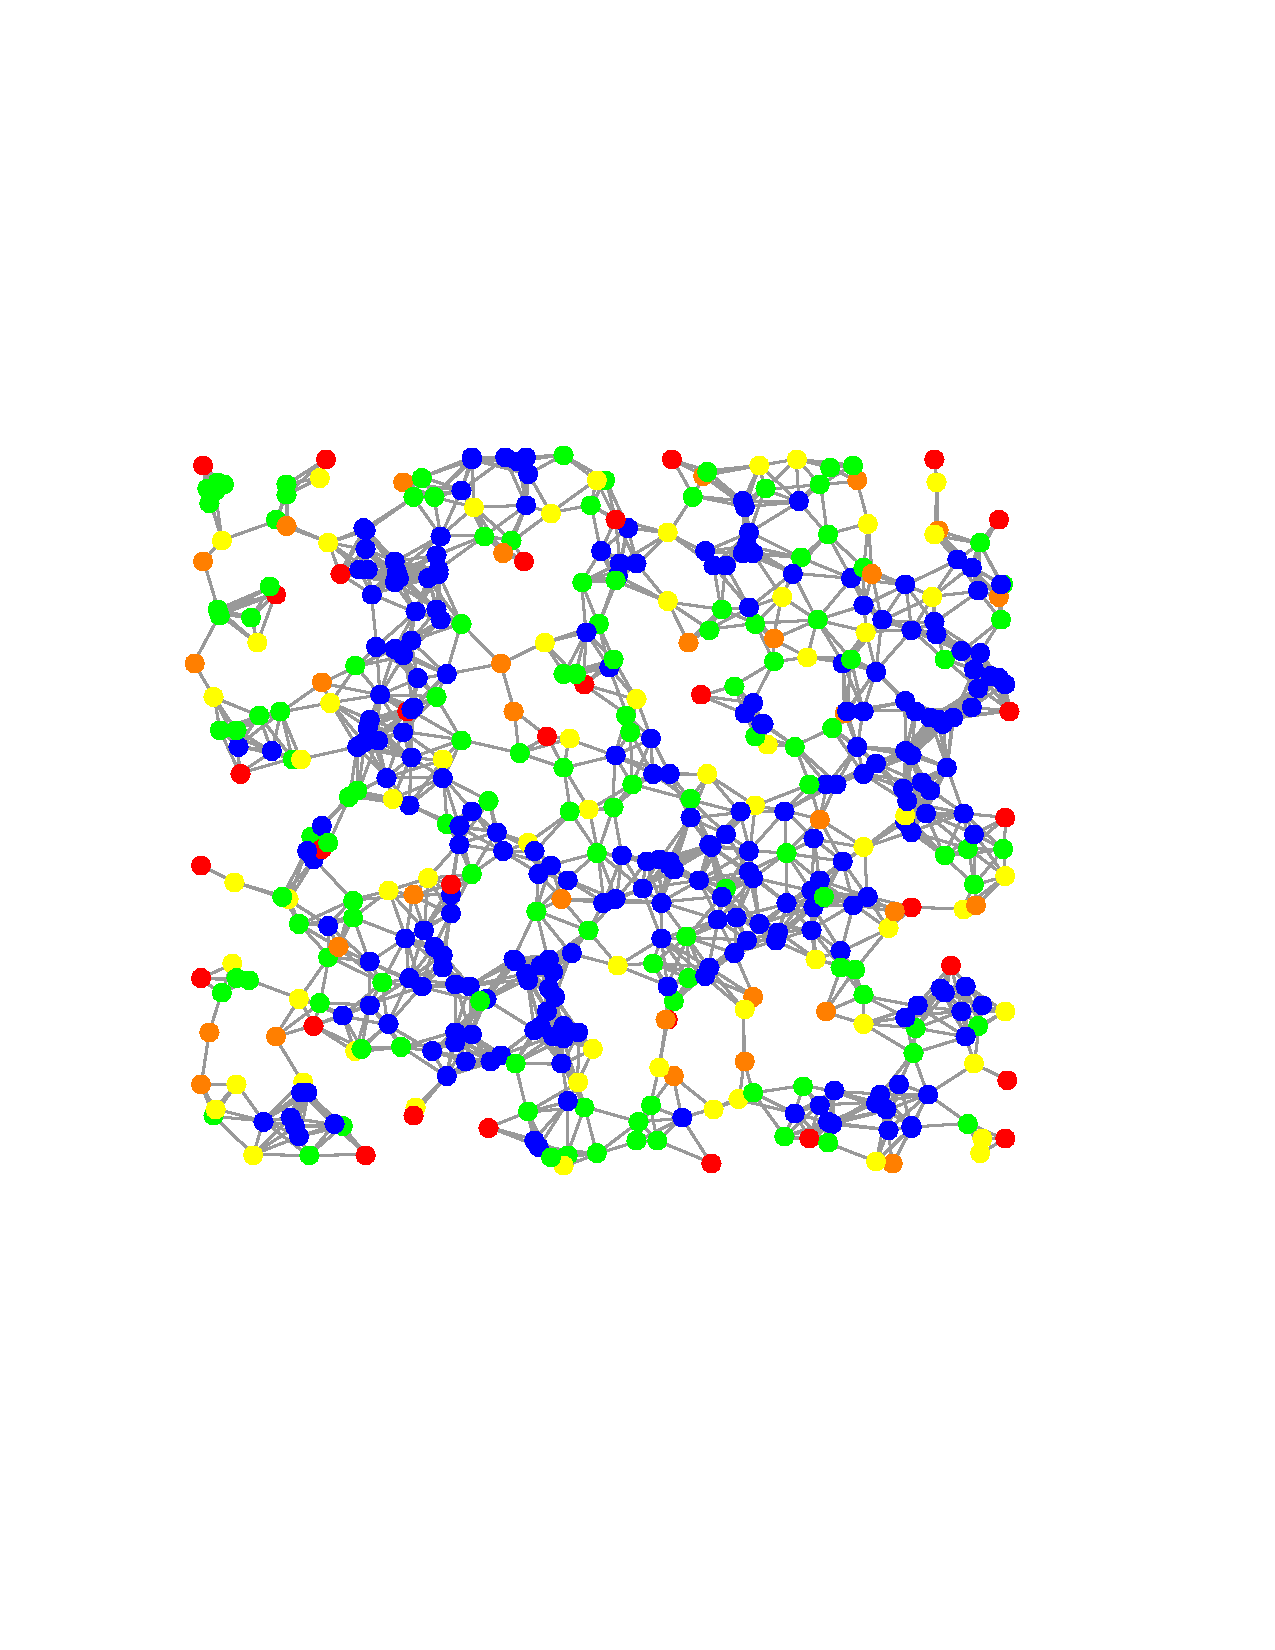
\includegraphics[width=.98\linewidth]{fig_uniq_part_sensor3}}
\end{minipage}
\hspace{.003\linewidth}
\begin{minipage}[m]{0.05\linewidth}
\centerline{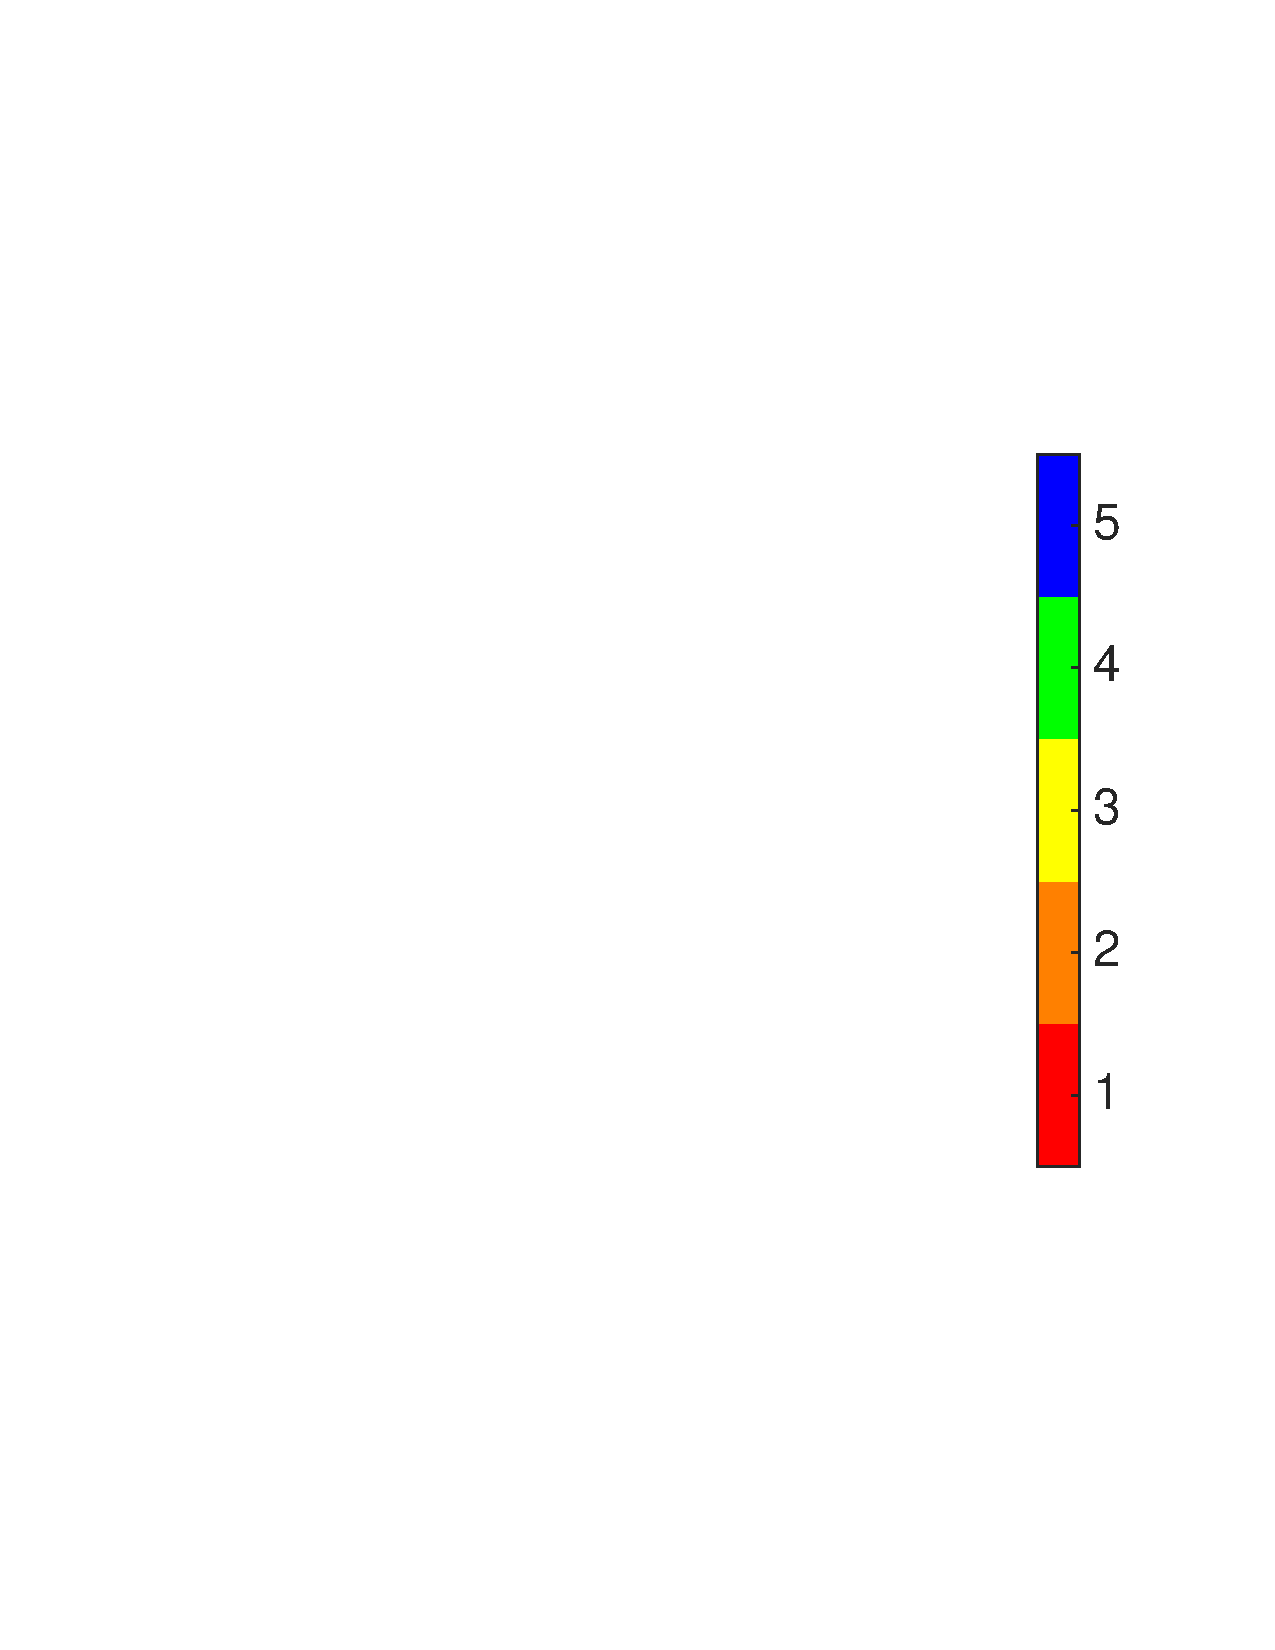
\includegraphics[width=.9\linewidth]{fig_uniq_part_col2}}
\end{minipage}
\hspace{.003\linewidth}
\begin{minipage}[m]{0.46\linewidth}
\centerline{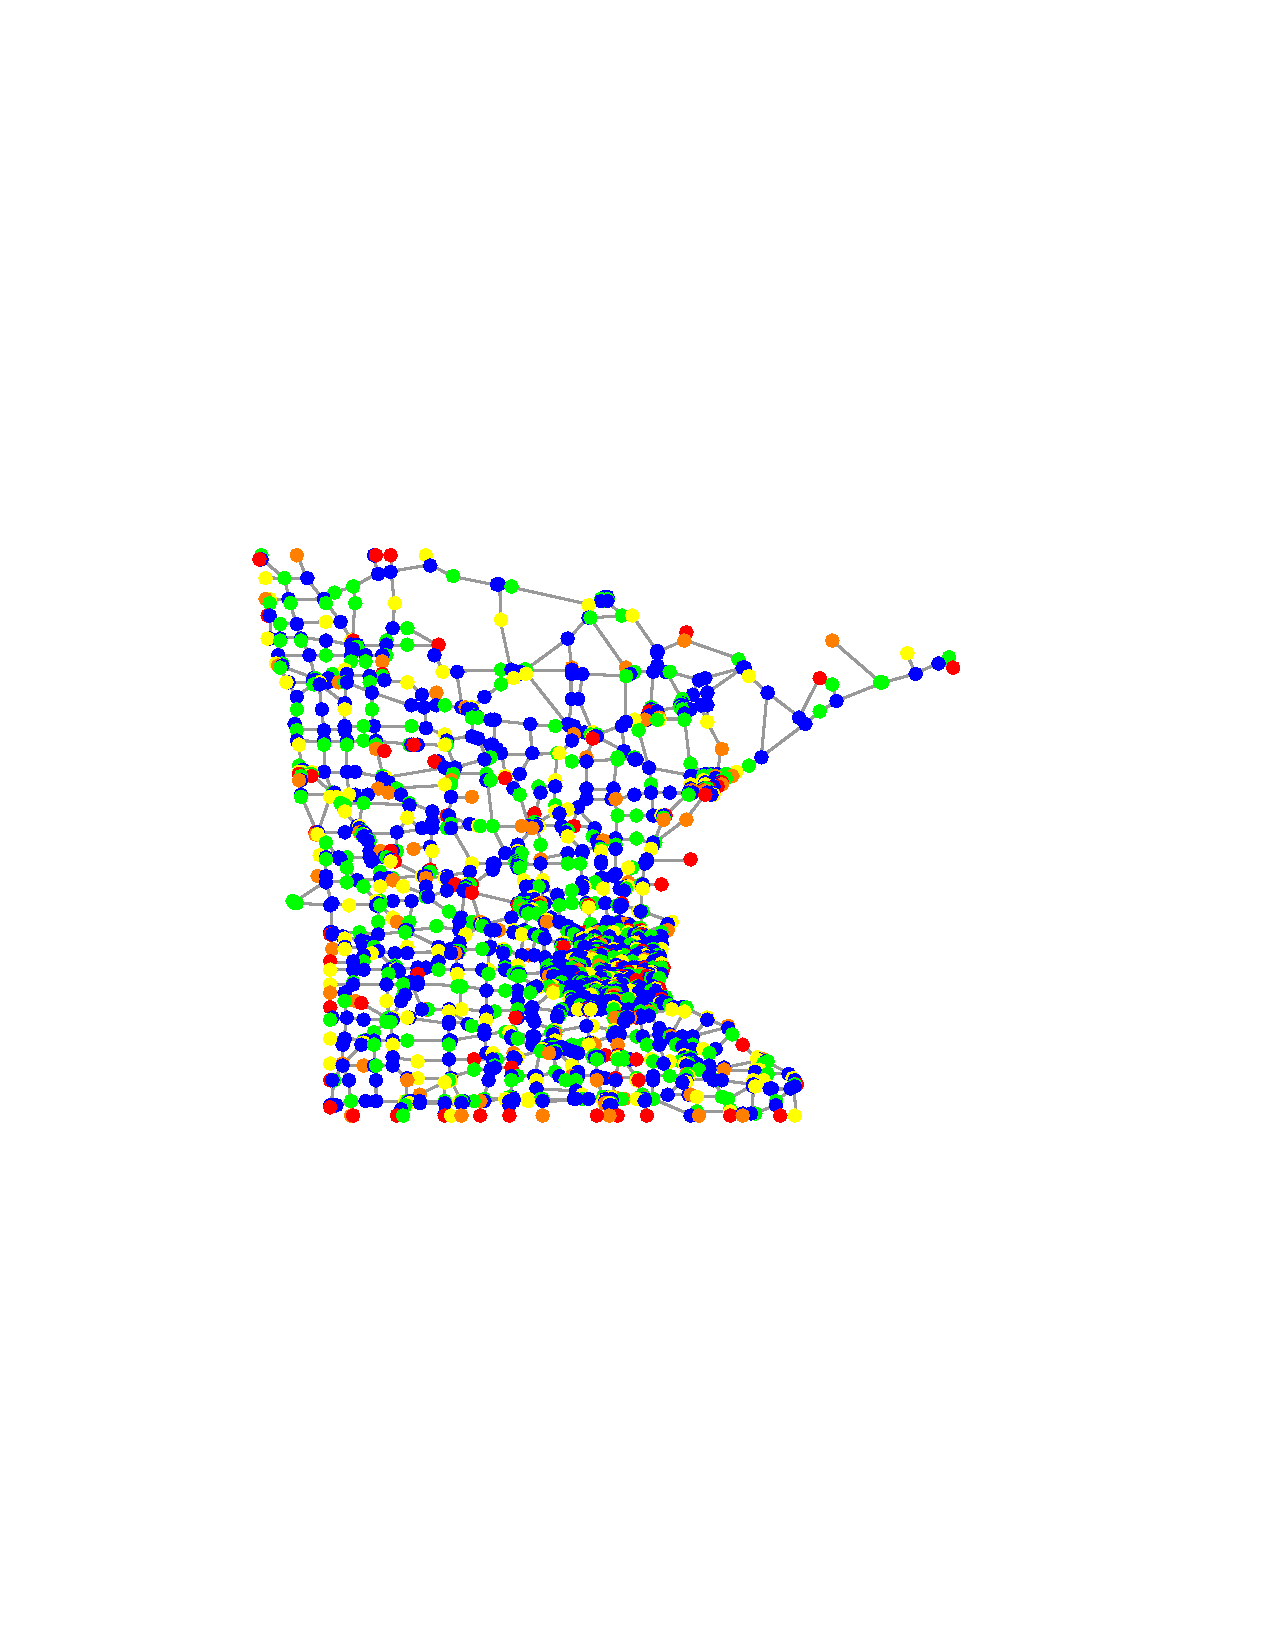
\includegraphics[width=\linewidth]{fig_uniq_part_minn4}}
\end{minipage}
\caption{Partitions of a 500 node random sensor network and the Minnesota road network \cite{gleich} into uniqueness sets for five different spectral bands, with the indices increasing from lowpass bands (1) to highpass bands (5).} \label{Fig:part_examples}
\end{figure} 


%\section{Dictionary Atoms and Signals that are Sparsely Represented by the MCSFB Transform}
\section{Transform Properties}
%{\color{red} Move this section until the end and discuss both the exact and approximate transforms together?}
We now briefly examine some properties of the proposed transform. 
\subsection{Dictionary atoms}
Let ${\bf M}_m \in \R^{|{\cal V}_m| \times N}$ be the downsampling matrix for the $m^{th}$ channel. That is, ${\bf M}_m(i,j)=1$ if vertex $j$ is the $i^{th}$ element of ${\cal V}_m$, and 0 otherwise. The proposed transform is a linear mapping ${\cal F}: \R^N \rightarrow \R^N$ by ${\cal F}{\bf f} = {\bf Tf}$, where 
\begin{align*}
{\bf T}=\left[
\begin{array}{c}
{\bf M}_1 h_1(\L) \\  \hdashline[.05cm/.05cm]
{\bf M}_2 h_2(\L) \\  \hdashline[.05cm/.05cm]
\vdots \\  \hdashline[.05cm/.05cm]
{\bf M}_M h_M(\L)
\end{array}
\right] \in \R^{N \times N}.
\end{align*}
The atoms of the resulting dictionary are given by the columns of ${\bf T}^{\top}$. While the transform is not orthogonal, each atom is orthogonal to all atoms concentrated on other spectral bands. Informally, this is because the atoms are projections of Kronecker deltas onto the orthogonal subspaces spanned by the Laplacian eigenvectors of each band. More formally, each atom is of the form $h_m(\L){\boldsymbol \delta}_i$, where vertex $i$ is in ${\cal V}_m$. If $m \neq m^{\prime}$, then the inner product of the two atoms from different bands is given by
\begin{align} \label{Eq:ortho_bands}
&\langle h_m(\L){\boldsymbol \delta}_i , h_{m^{\prime}}(\L){\boldsymbol \delta}_{i^{\prime}} \rangle \nonumber \\
&~~~~~~= {\boldsymbol \delta}_i^{\top} {\bf U} h_m({\boldsymbol \Lambda}) {\bf U}^* {\bf U} h_{m^{\prime}}({\boldsymbol \Lambda}) {\bf U}^* {\boldsymbol \delta}_{i^{\prime}}= 0,
\end{align}
since ${\bf U}^* {\bf U}={\bf I}$ and $h_m(\lambda)h_{m^{\prime}}(\lambda)=0$ for all $\lambda$ by design.
%One possible extension is to find a fast algorithm to orthogonalize the atoms within each band. 
Note also that the wavelet atoms at all scales ($m>1$) have mean zero, as they have no energy at eigenvalue zero.

{\color{red}

\subsection{Signals that are sparsely represented by the M-CSFB transform}
\begin{itemize}
%\item Add theorem about orthogonality across bands
\item Concentrated in the graph Fourier domain
\item If spectral coefficients decay, transform coefficients also decay
\item Characterization of joint localization? Localization in vertex domain guaranteed when polynomial filters used
\item We  plan to more formally characterize the relationships between the decay of the analysis coefficients under the proposed transform and different properties of graph signals, as well as the underlying graph structure.
Globally smooth signals trivially lead to sparse analysis coefficients because the coefficients are only nonzero for first set of vertices in the partition. The same line of reasoning applies more generally to signals that are sparse in the graph spectral domain. More interesting is a theory for the coefficient decay for piecewise-smooth graph signals such as the ones shown in Fig. \ref{Fig:bunny_signal}(a) and Fig. \ref{Fig:comp}(a).
\end{itemize}
%\subsection{Computational complexity}
}

\section{Illustrative Examples I: Exact Calculations}
We can represent the proposed filter bank as an $N \times N$ dictionary matrix $\boldsymbol{\Phi}$ that maps graph signals to their filter bank analysis coefficients. 

\begin{figure*}[bth] 
\begin{minipage}[m]{0.16\linewidth}
~
\end{minipage}
\begin{minipage}[m]{0.16\linewidth}
\centerline{\small{Scaling Functions}}
\end{minipage}
\hspace{.01\linewidth}
\begin{minipage}[m]{0.16\linewidth}
\centerline{\small{Wavelet Scale 1~~~~}}
\end{minipage}
\begin{minipage}[m]{0.16\linewidth}
\centerline{\small{Wavelet Scale 2~~~~}}\end{minipage}
\begin{minipage}[m]{0.16\linewidth}
\centerline{\small{Wavelet Scale 3~~~~}}\end{minipage}
\begin{minipage}[m]{0.16\linewidth}
\centerline{\small{Wavelet Scale 4~~~~~}}\end{minipage} \\
\begin{minipage}[m]{0.16\linewidth}
\centerline{\small{Example Atom}}
\end{minipage}
\begin{minipage}[m]{0.16\linewidth}
\centerline{~~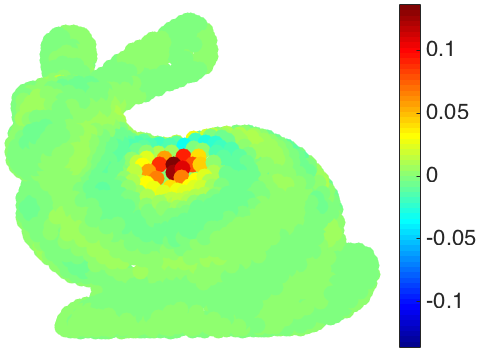
\includegraphics[width=.85\linewidth]{fig_bunny_atom_scalinga}}
\end{minipage}
\begin{minipage}[m]{0.16\linewidth}
\centerline{~~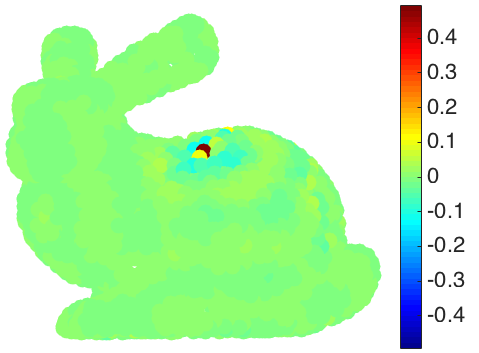
\includegraphics[width=.85\linewidth]{fig_bunny_atom_wav1a}}
\end{minipage}
\begin{minipage}[m]{0.16\linewidth}
\centerline{~~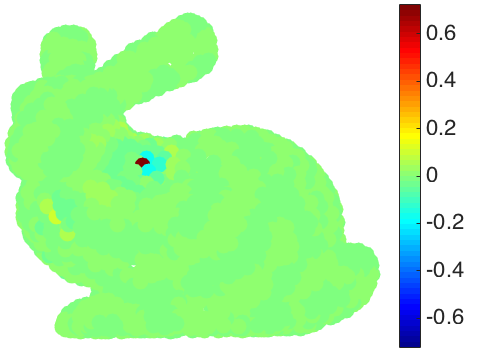
\includegraphics[width=.85\linewidth]{fig_bunny_atom_wav2a}}
\end{minipage}
\begin{minipage}[m]{0.16\linewidth}
\centerline{~~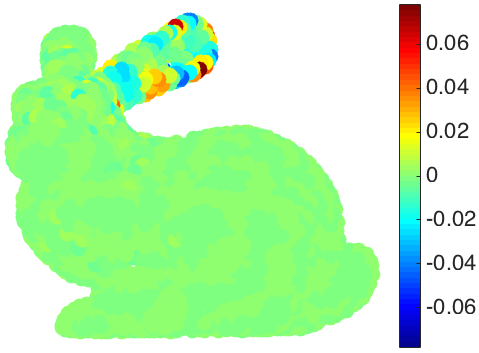
\includegraphics[width=.85\linewidth]{fig_bunny_atom_wav3a}}
\end{minipage}
\begin{minipage}[m]{0.16\linewidth}
\centerline{~~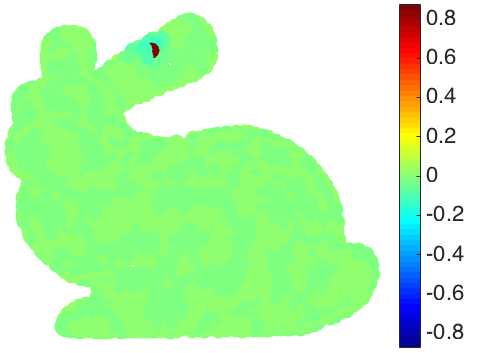
\includegraphics[width=.85\linewidth]{fig_bunny_atom_wav4a}}
\end{minipage}\\
\begin{minipage}[m]{0.16\linewidth}
\centerline{\small{Spectral Content}}
\centerline{\small{of All Atoms}}
\end{minipage}
\begin{minipage}[m]{0.16\linewidth}
\centerline{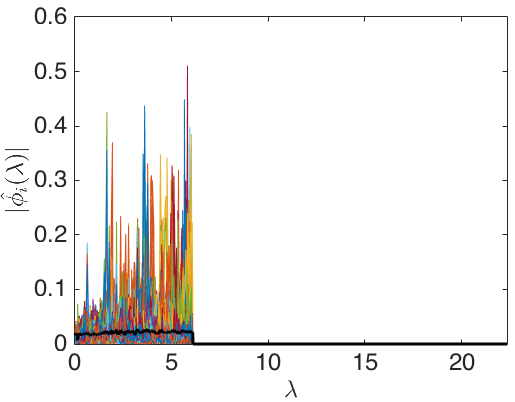
\includegraphics[width=.8\linewidth]{fig_bunny_freq_scaling3}}
\end{minipage}
\begin{minipage}[m]{0.16\linewidth}
\centerline{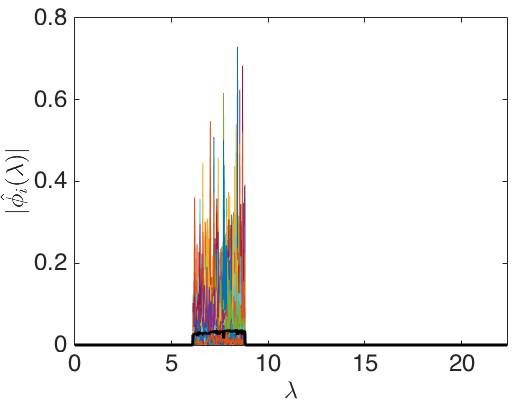
\includegraphics[width=.8\linewidth]{fig_bunny_freq_wav1a}}
\end{minipage}
\begin{minipage}[m]{0.16\linewidth}
\centerline{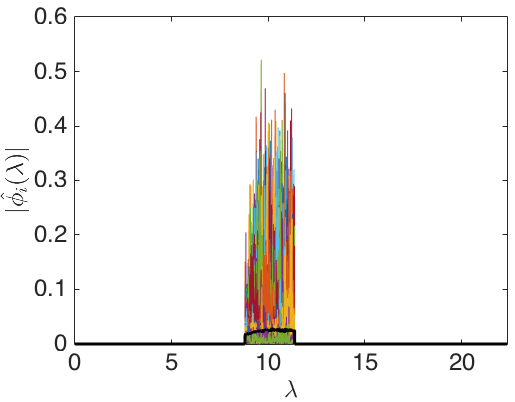
\includegraphics[width=.8\linewidth]{fig_bunny_freq_wav2a}}
\end{minipage}
\begin{minipage}[m]{0.16\linewidth}
\centerline{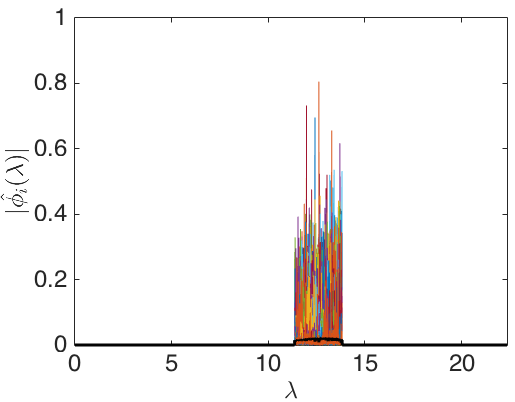
\includegraphics[width=.8\linewidth]{fig_bunny_freq_wav3a}}
\end{minipage}
\begin{minipage}[m]{0.16\linewidth}
\centerline{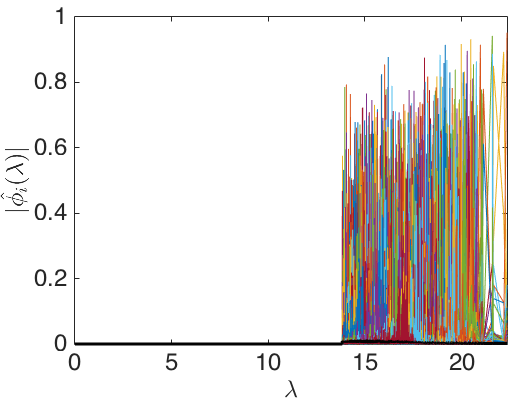
\includegraphics[width=.8\linewidth]{fig_bunny_freq_wav4a}}
\end{minipage}\\
\begin{minipage}[m]{0.16\linewidth}
\centerline{\small{Analysis}}
\centerline{\small{Coefficients}}
\end{minipage}
\begin{minipage}[m]{0.16\linewidth}
\centerline{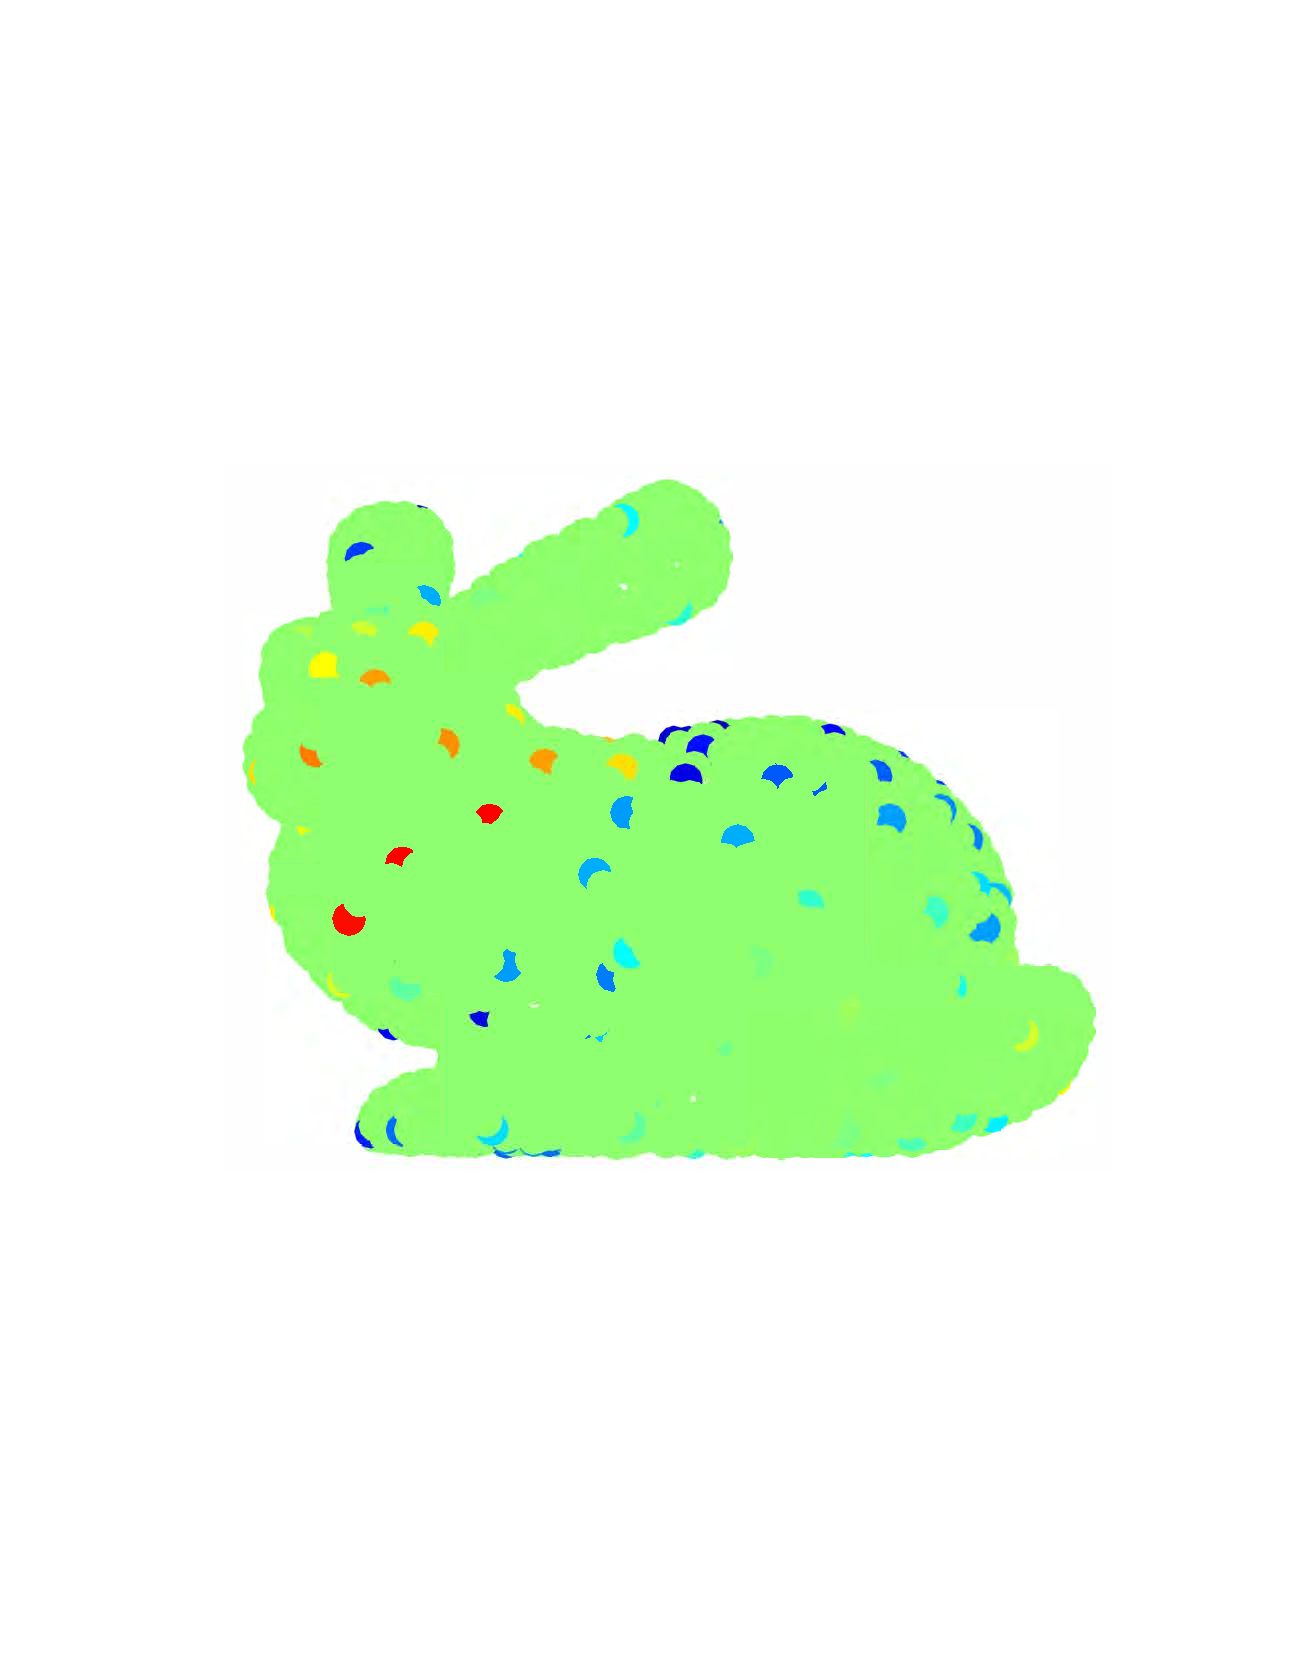
\includegraphics[width=.8\linewidth]{fig_bunny_coef_scaling}}
\end{minipage}
\begin{minipage}[m]{0.16\linewidth}
\centerline{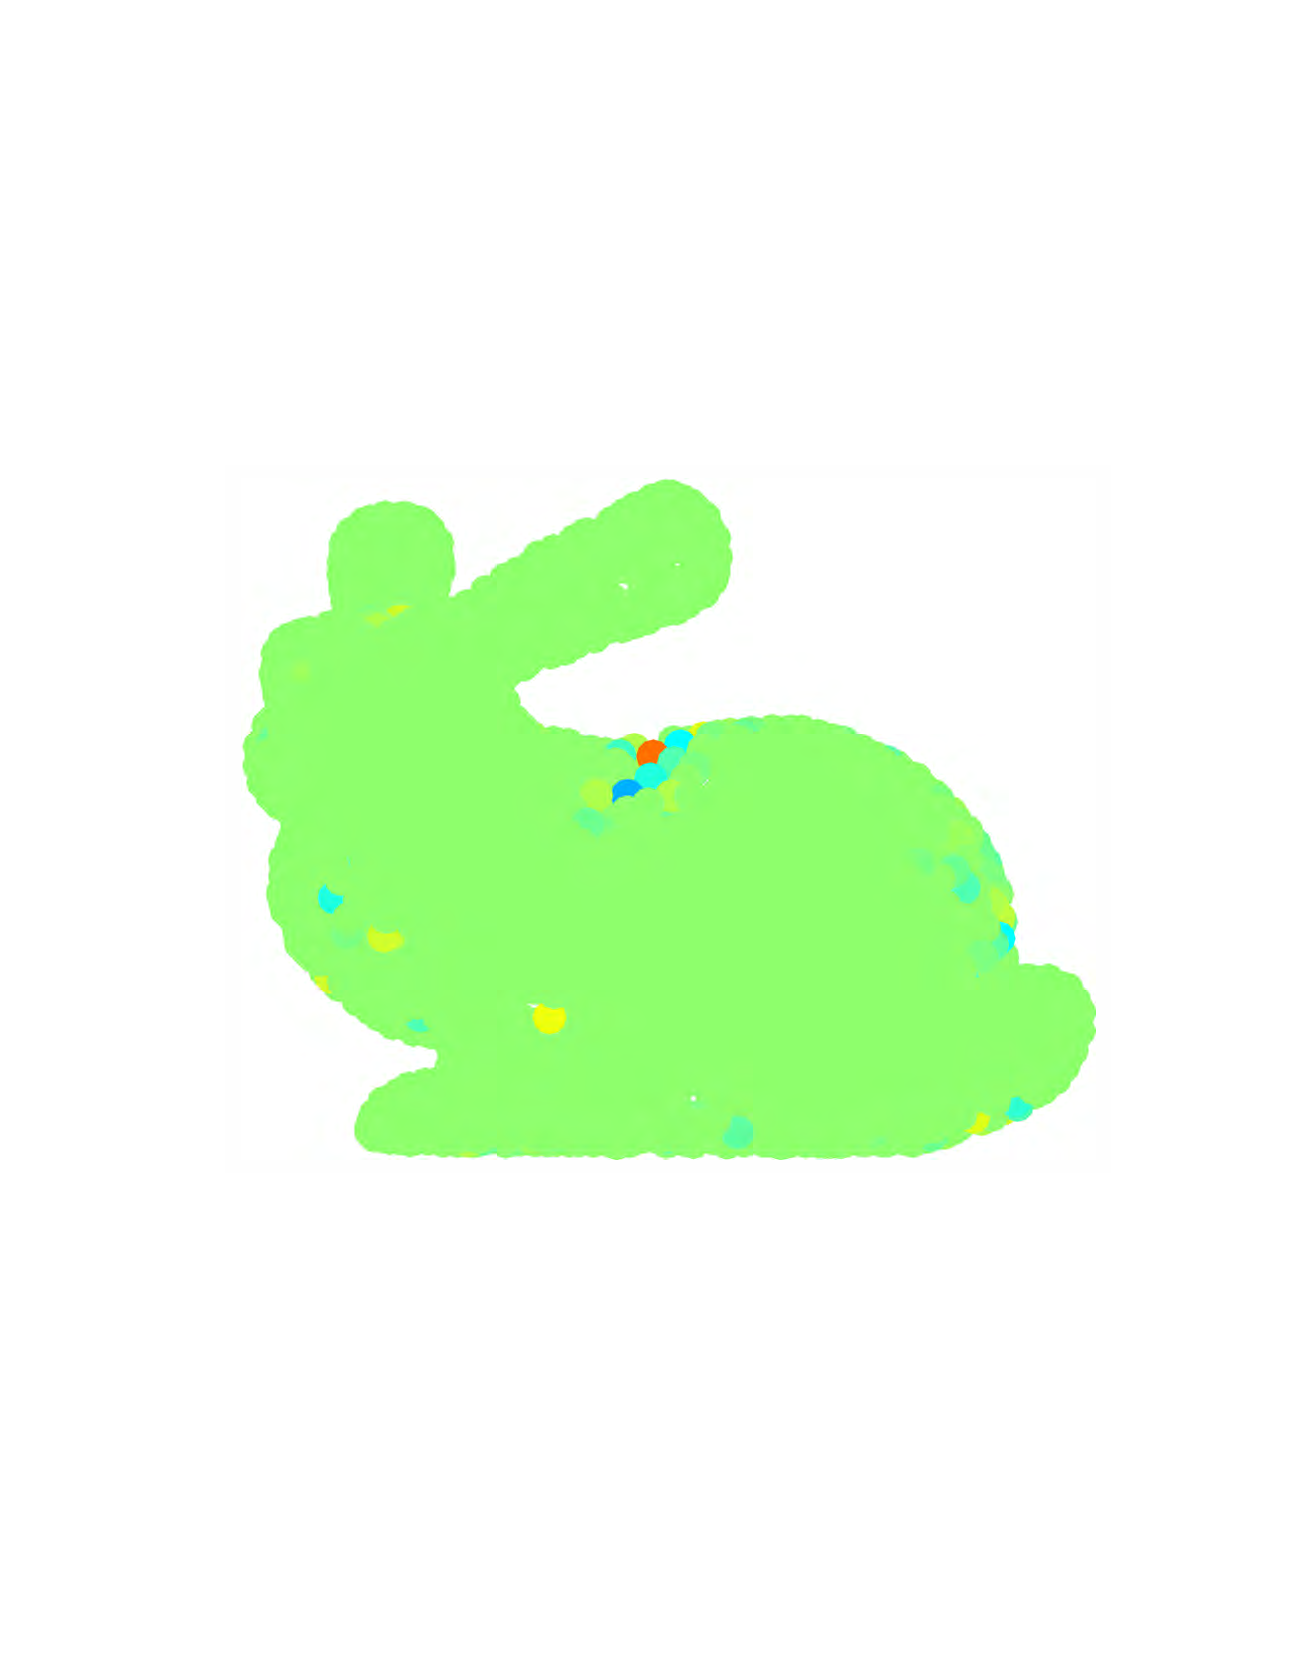
\includegraphics[width=.8\linewidth]{fig_bunny_coef_wav1}}
\end{minipage}
\begin{minipage}[m]{0.16\linewidth}
\centerline{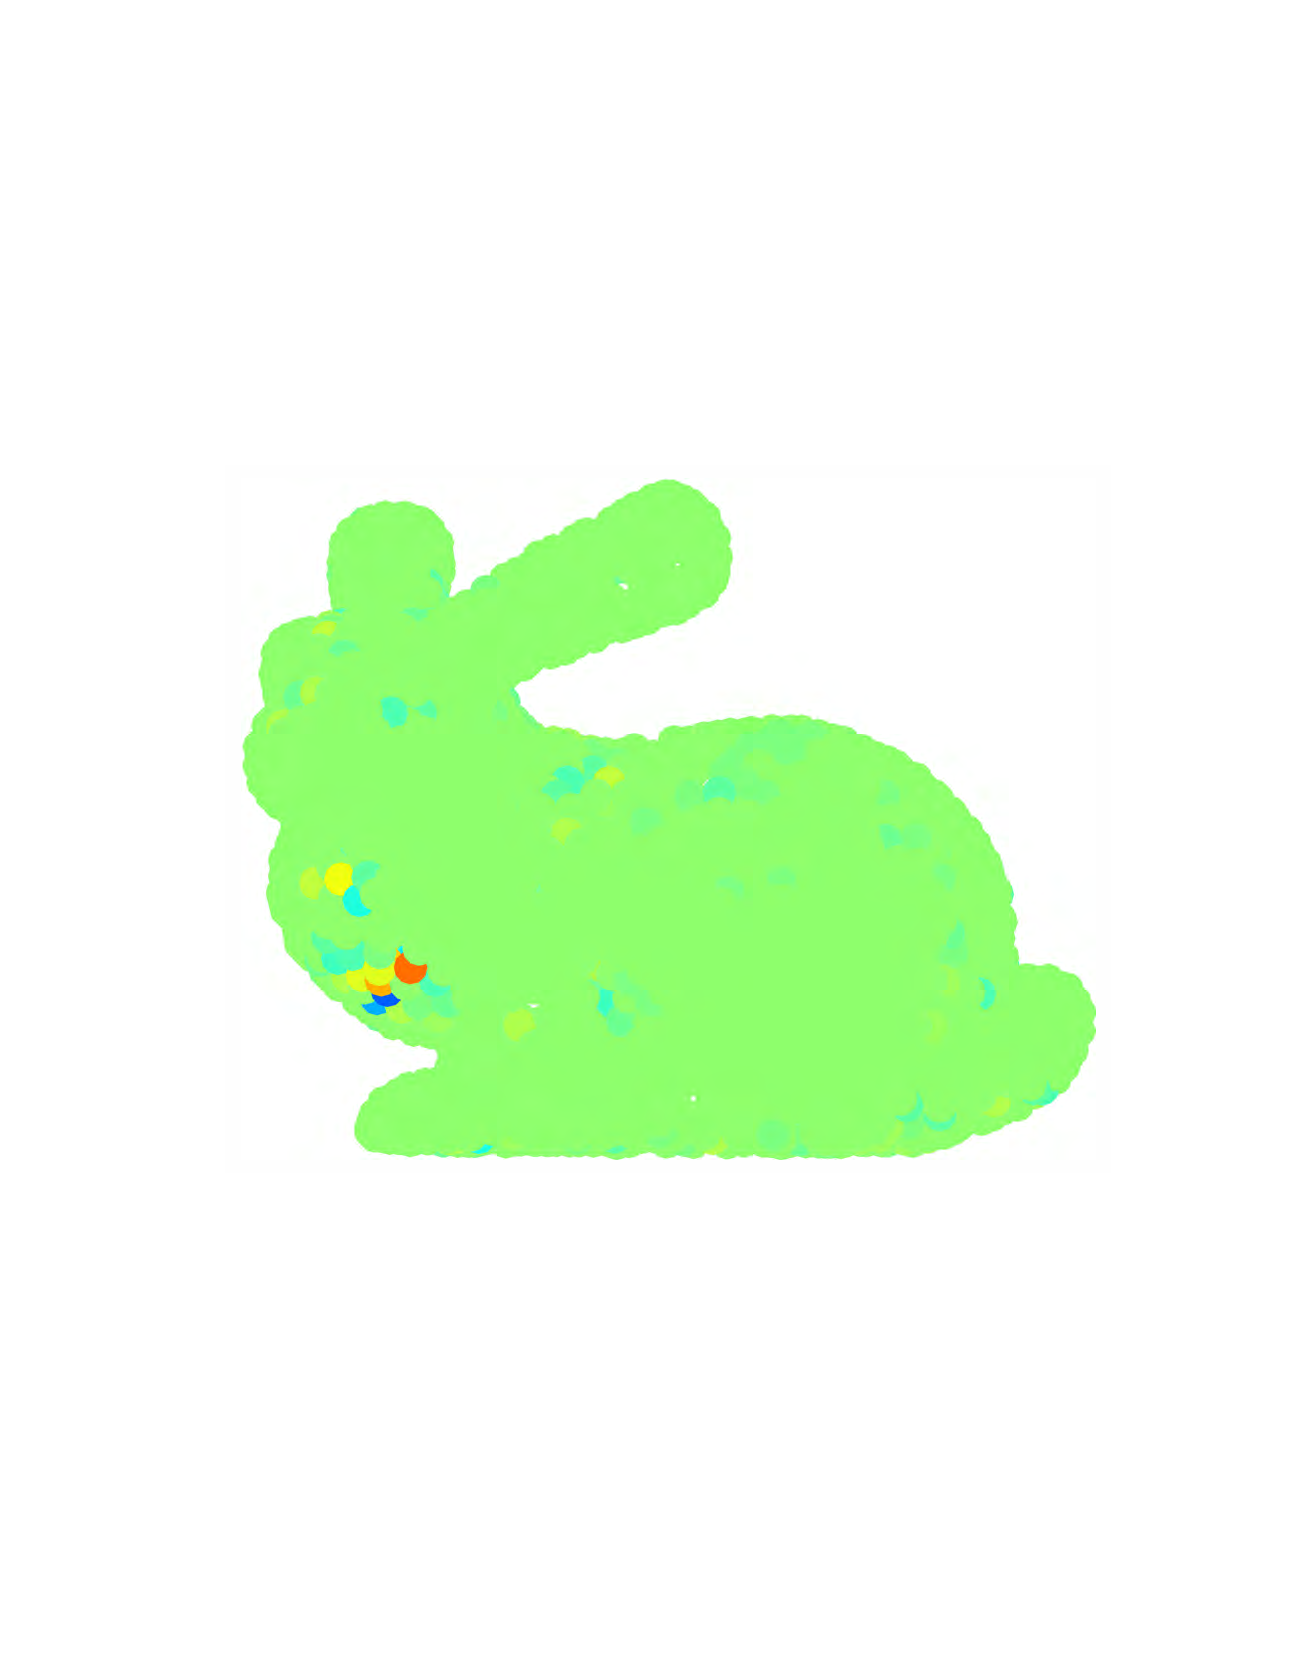
\includegraphics[width=.8\linewidth]{fig_bunny_coef_wav2}}
\end{minipage}
\begin{minipage}[m]{0.16\linewidth}
\centerline{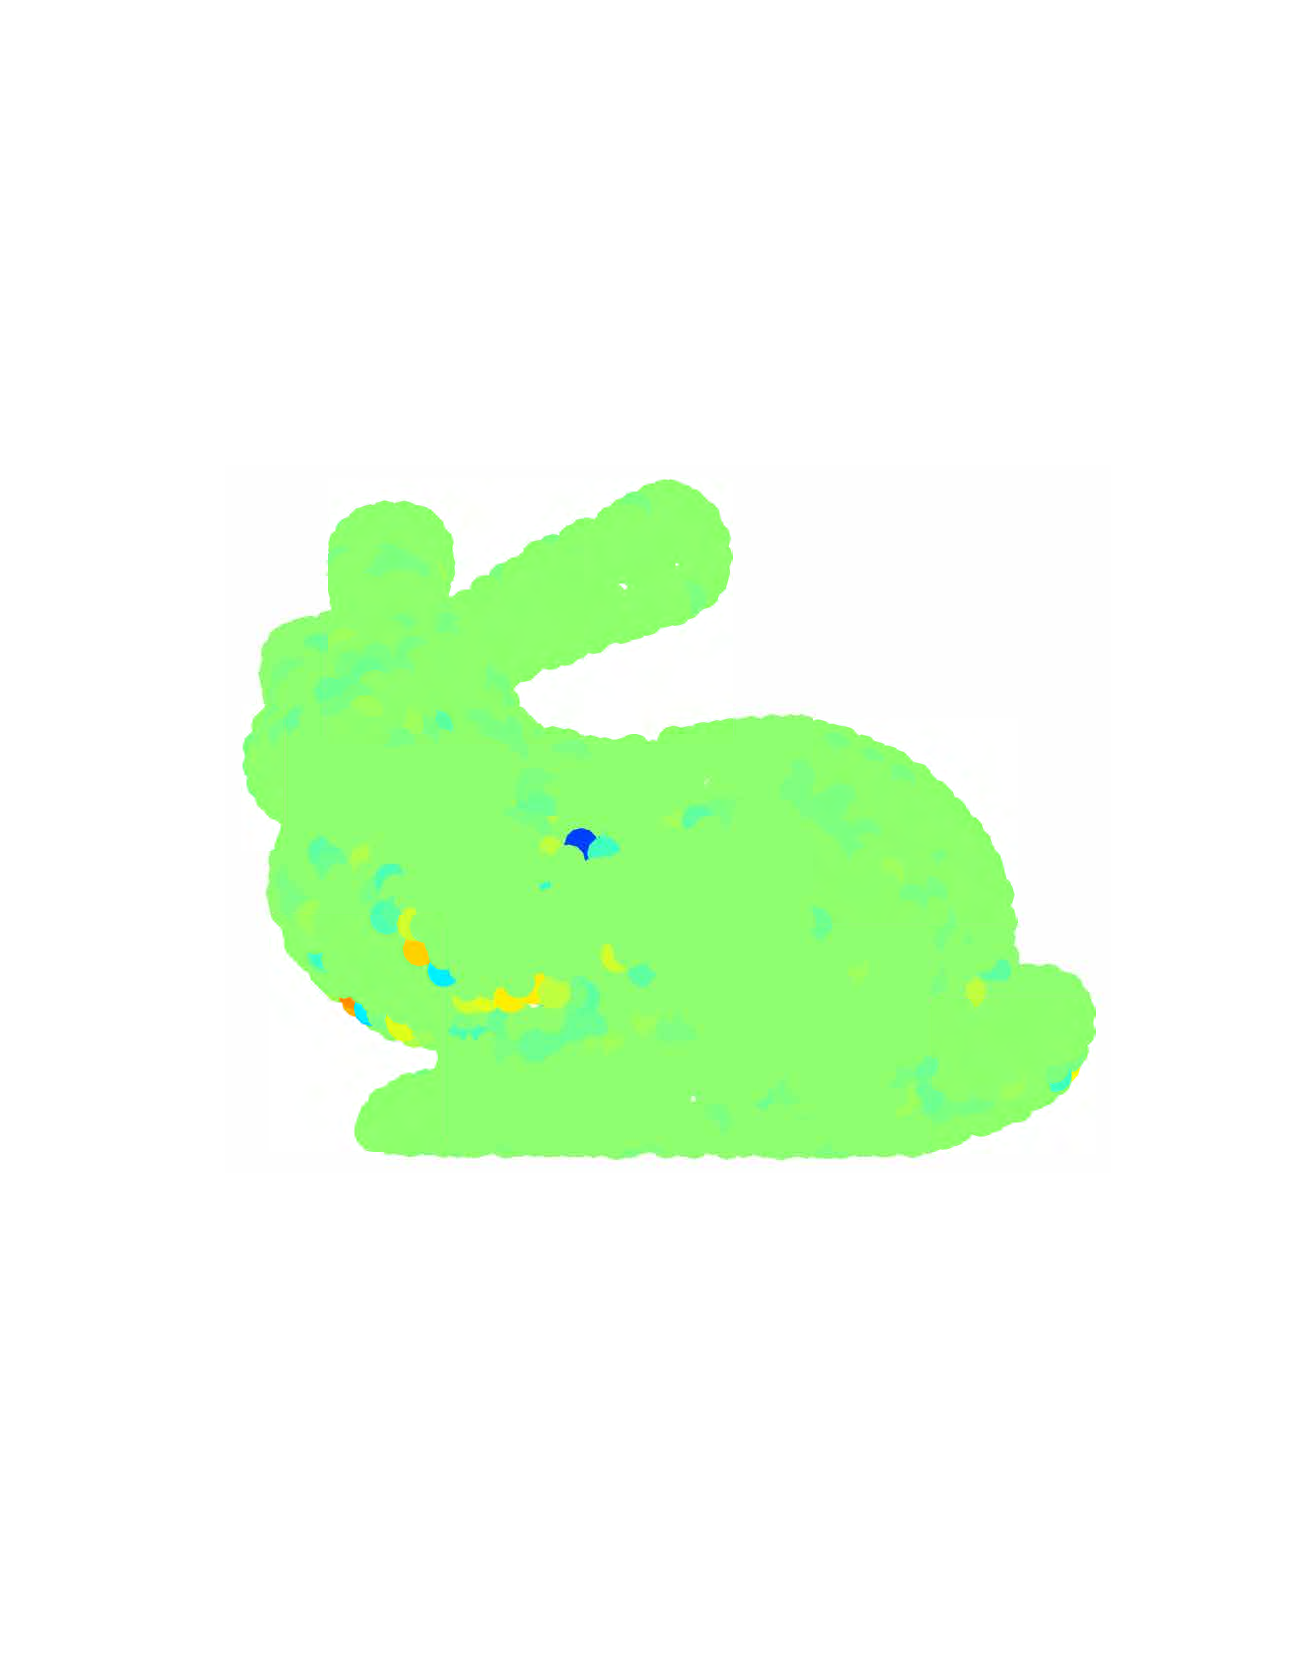
\includegraphics[width=.8\linewidth]{fig_bunny_coef_wav3}}
\end{minipage}
\begin{minipage}[m]{0.16\linewidth}
\centerline{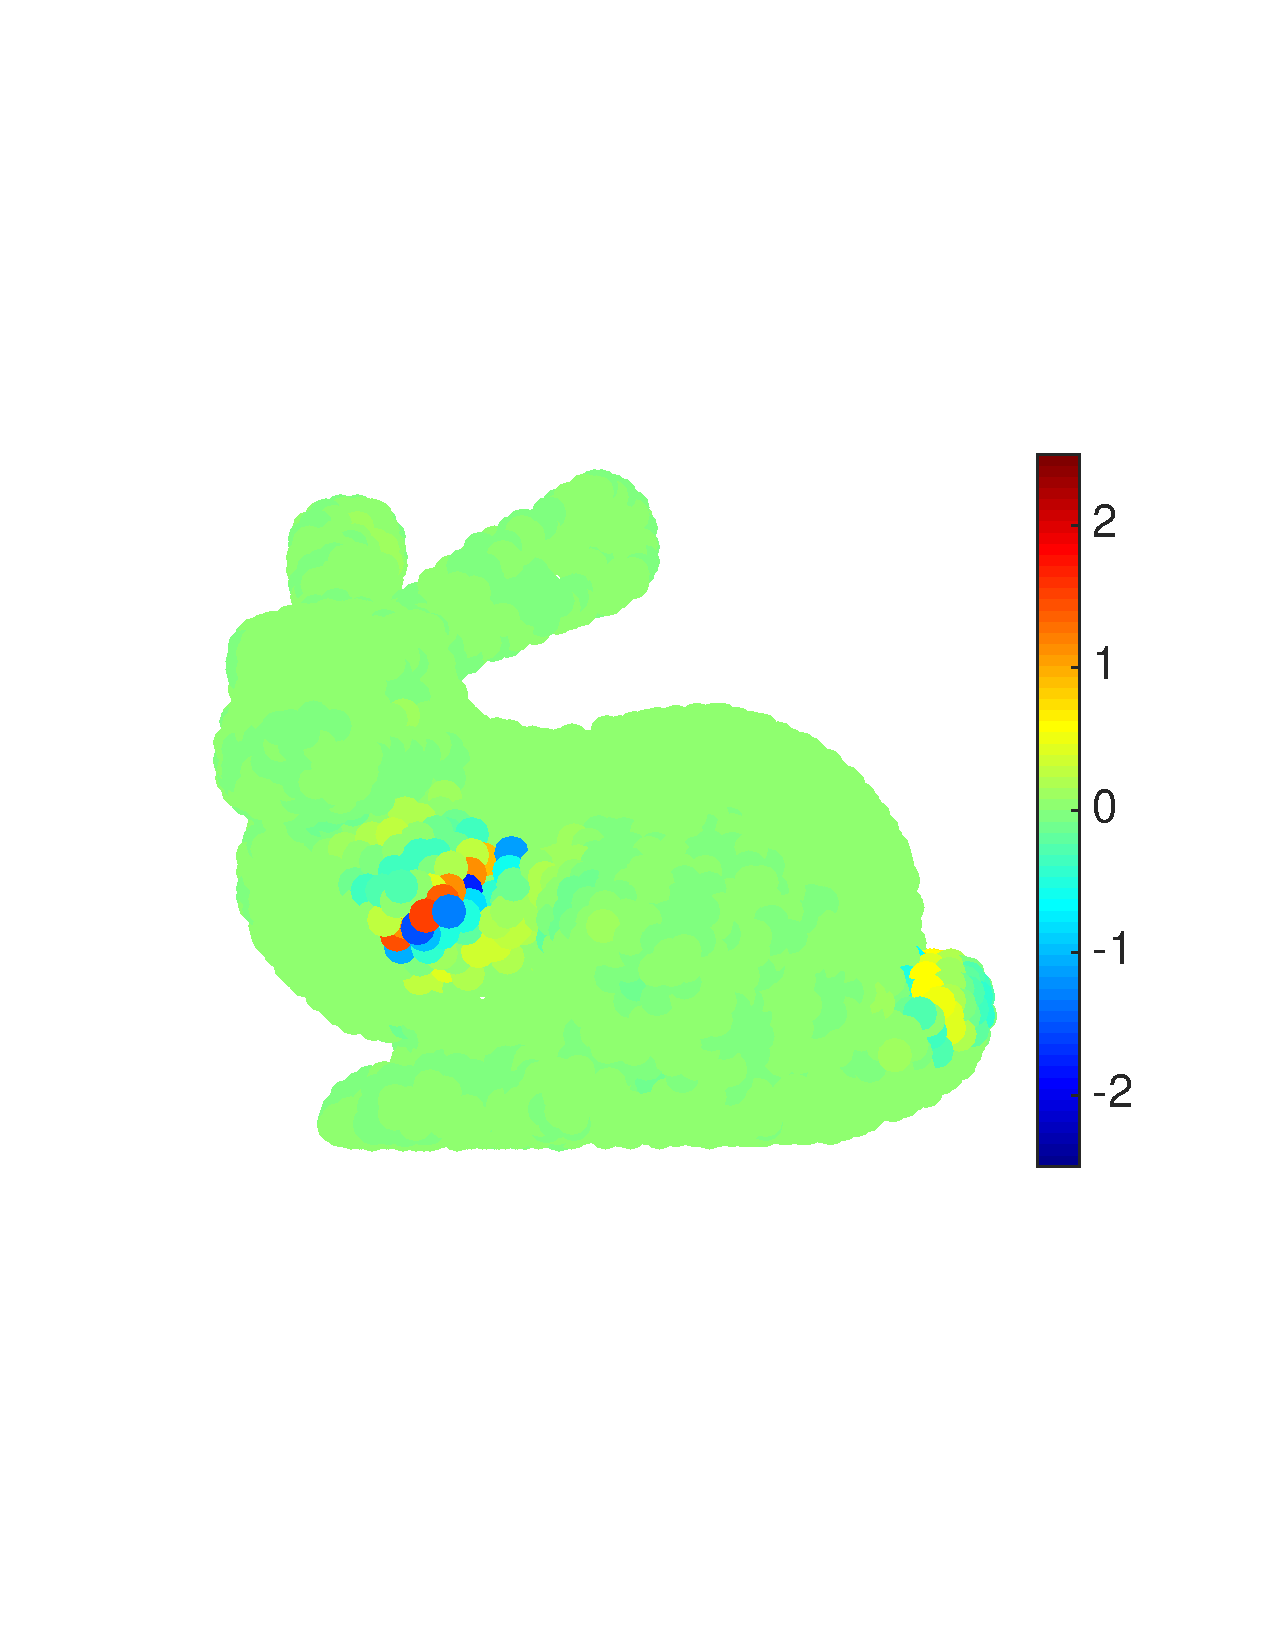
\includegraphics[width=.85\linewidth]{fig_bunny_coef_wav4}}
\end{minipage}\\
\begin{minipage}[m]{0.16\linewidth}
\centerline{\small{Reconstruction}}
\centerline{\small{by Band}}
\end{minipage}
\begin{minipage}[m]{0.16\linewidth}
\centerline{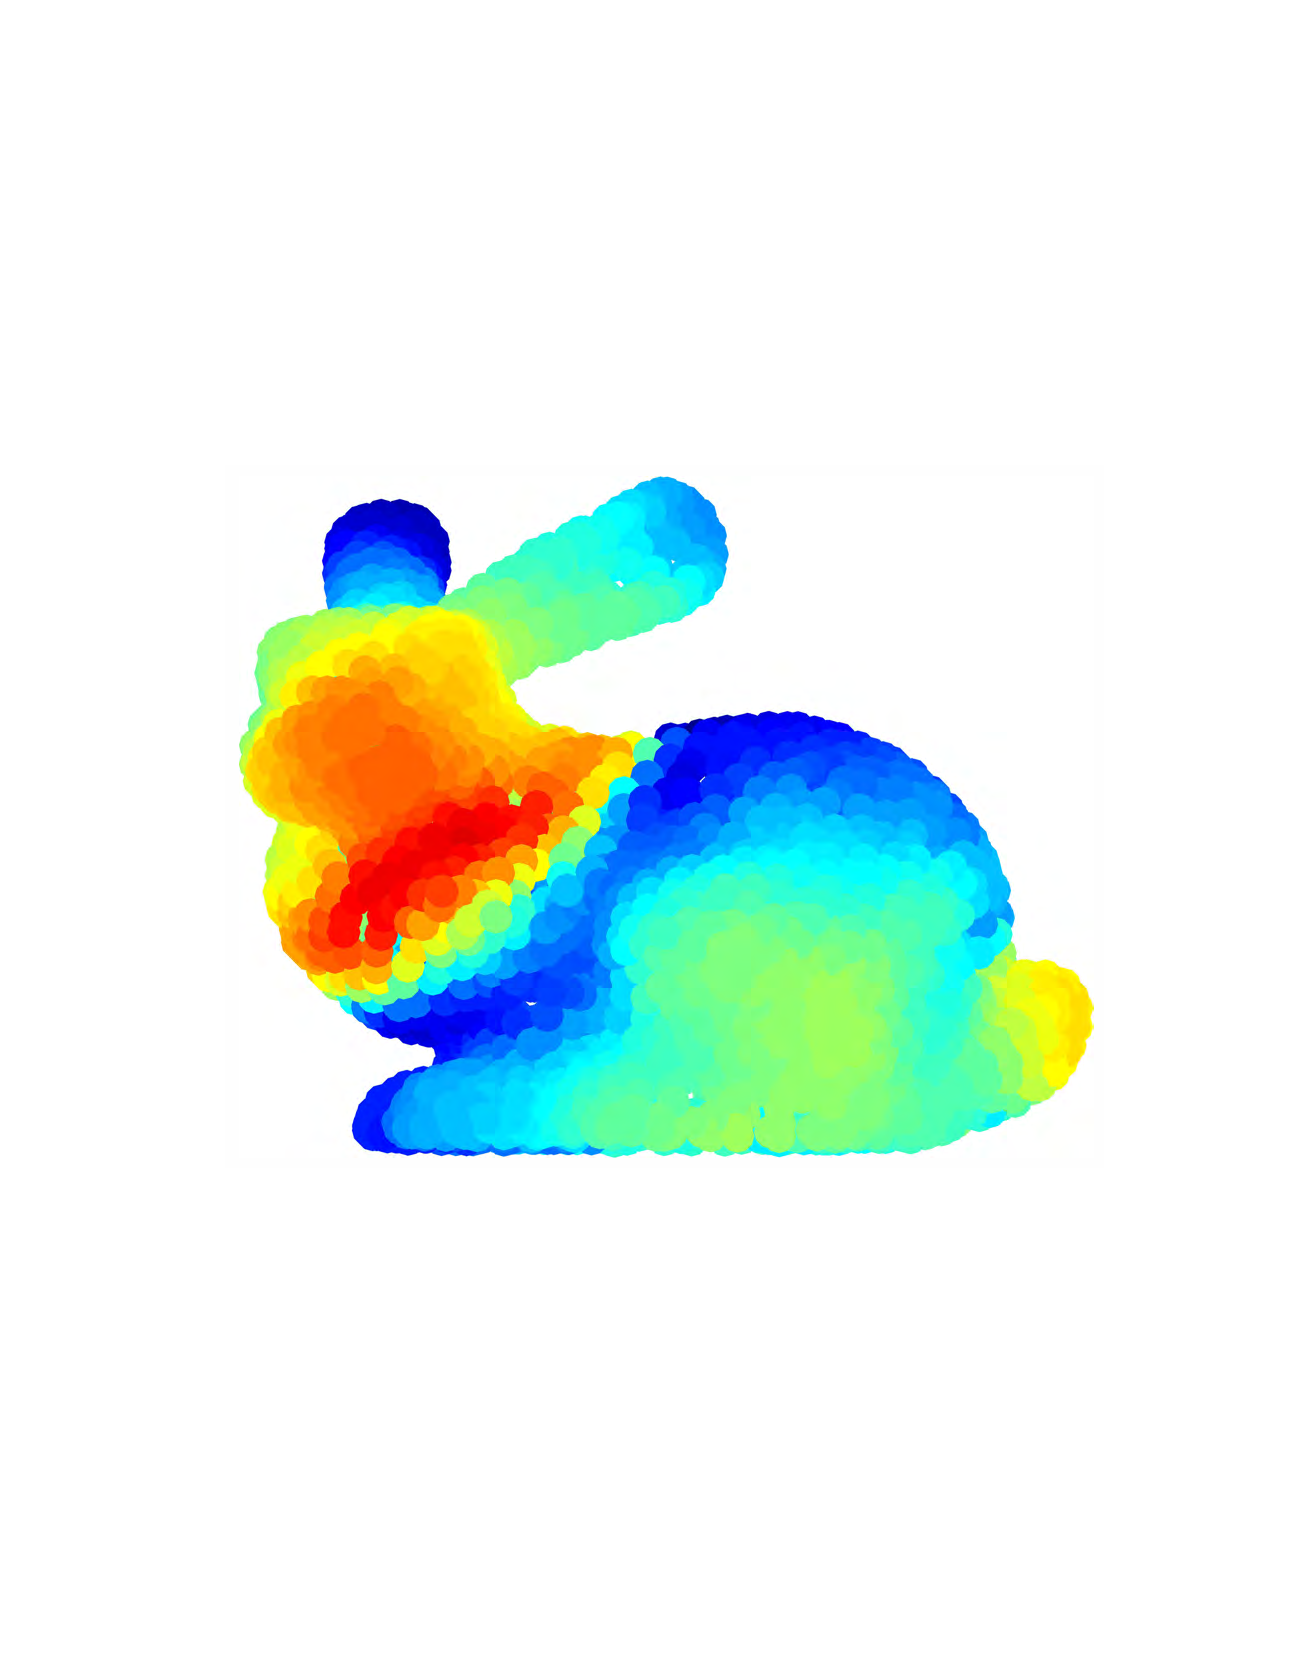
\includegraphics[width=.8\linewidth]{fig_bunny_rec_scaling}}
\end{minipage}
\begin{minipage}[m]{0.16\linewidth}
\centerline{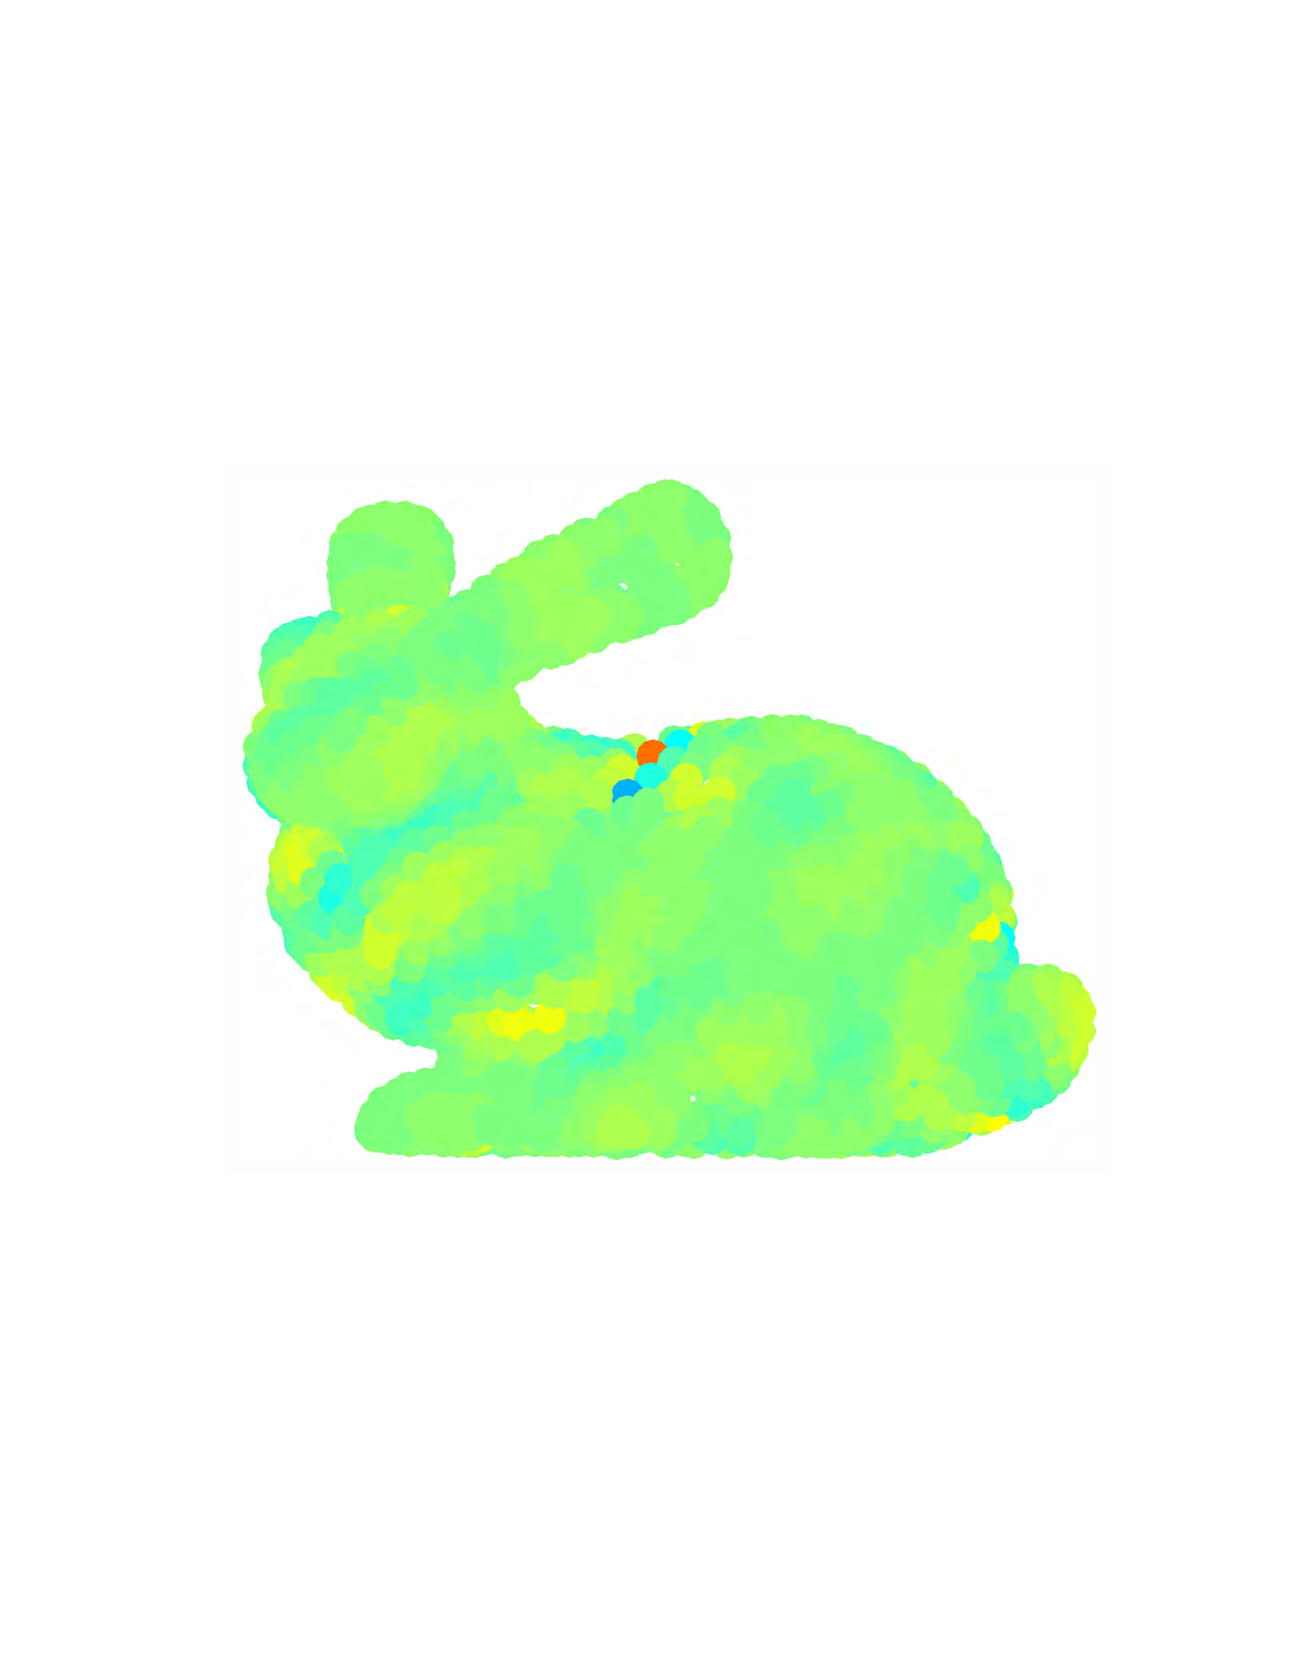
\includegraphics[width=.8\linewidth]{fig_bunny_rec_wav1}}
\end{minipage}
\begin{minipage}[m]{0.16\linewidth}
\centerline{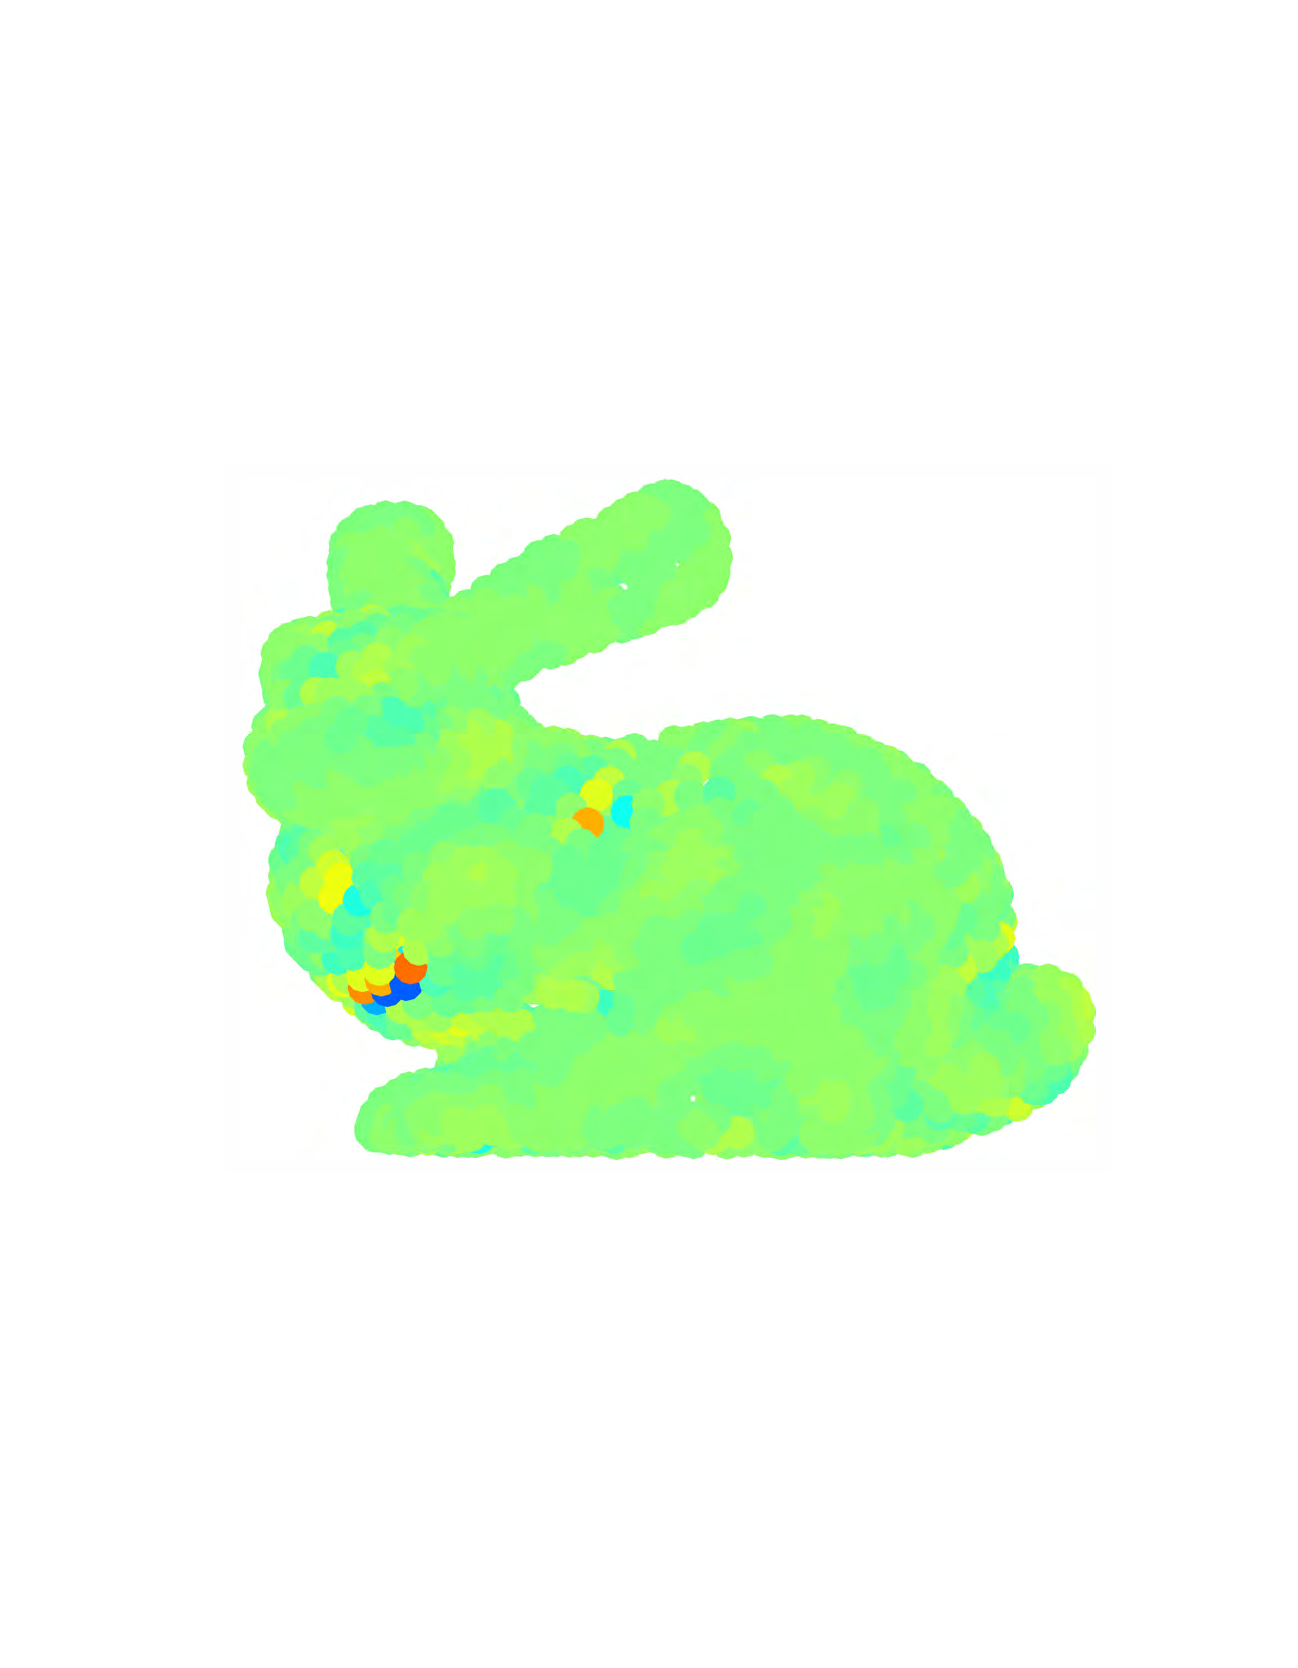
\includegraphics[width=.8\linewidth]{fig_bunny_rec_wav2}}
\end{minipage}
\begin{minipage}[m]{0.16\linewidth}
\centerline{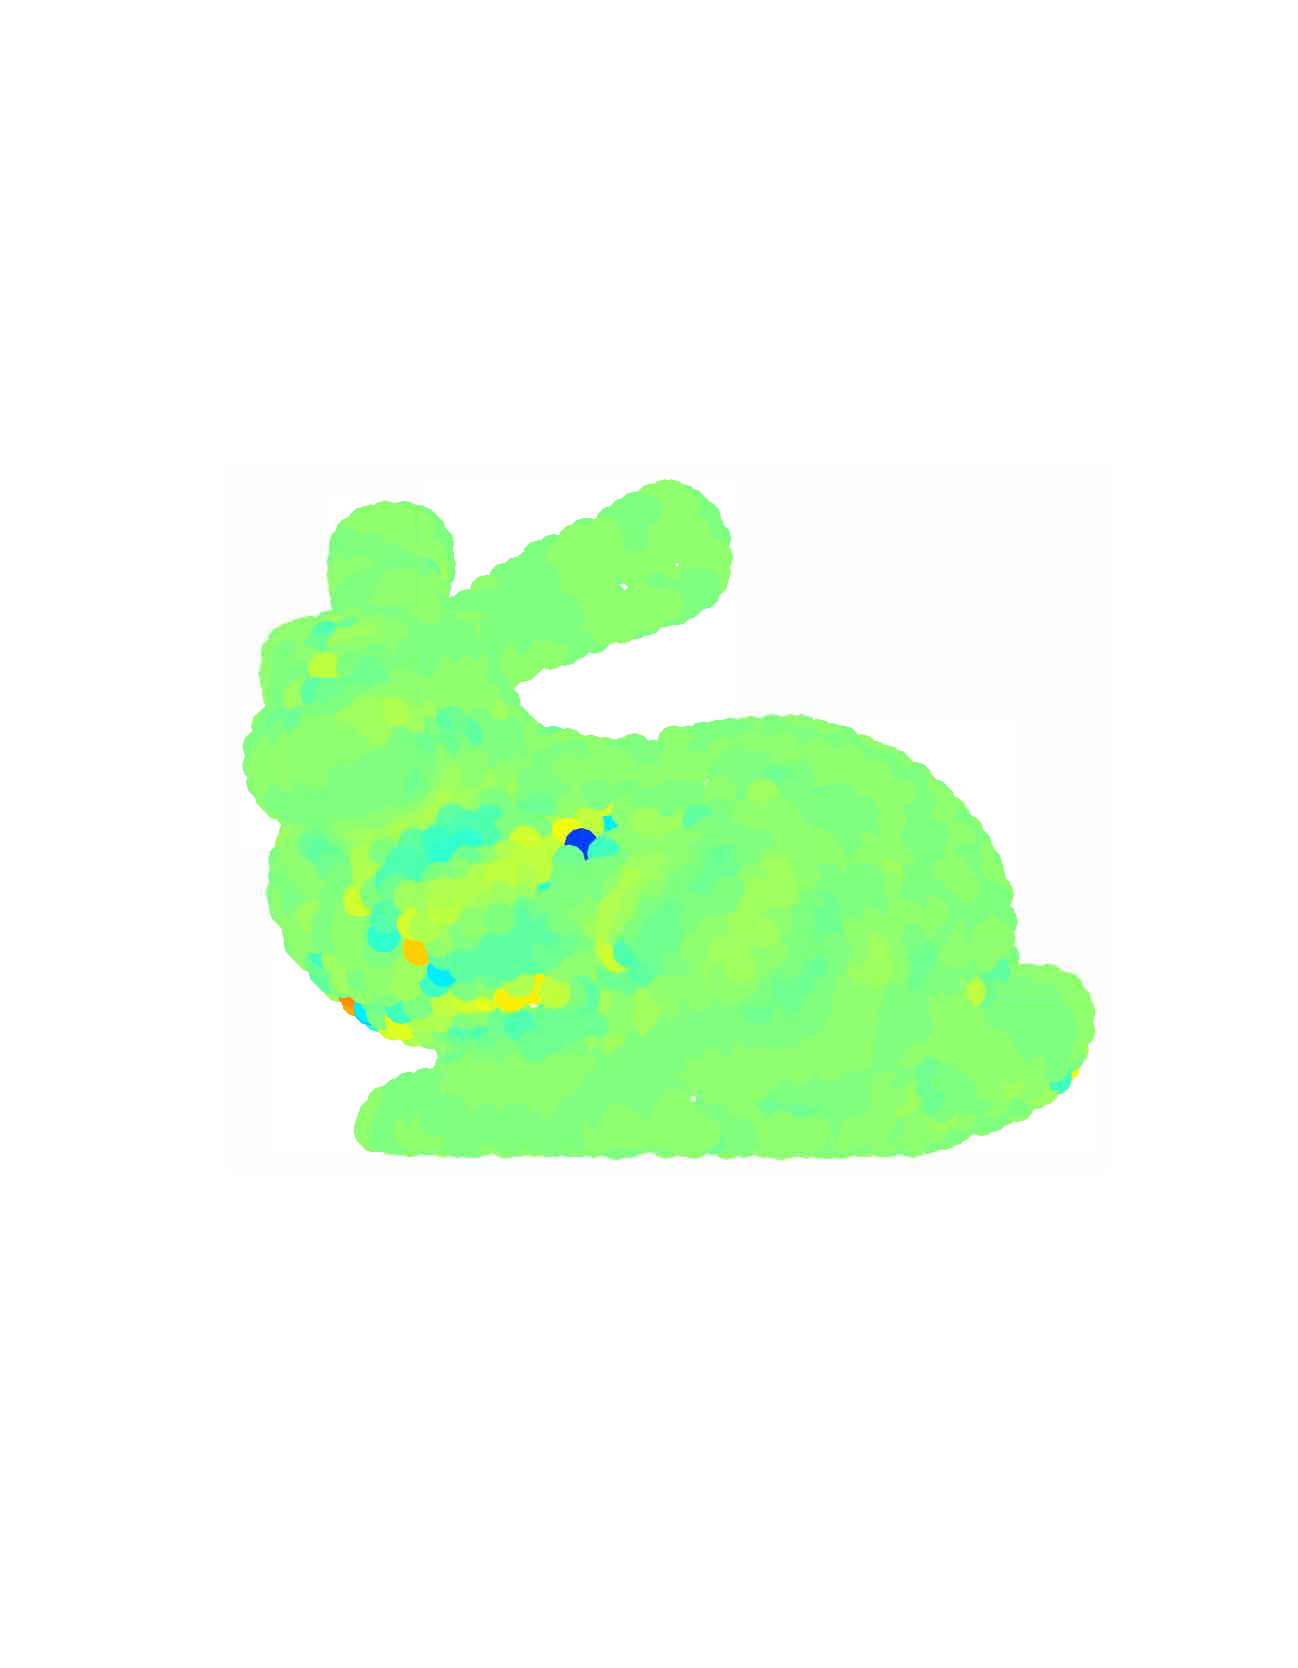
\includegraphics[width=.8\linewidth]{fig_bunny_rec_wav3}}
\end{minipage}
\begin{minipage}[m]{0.16\linewidth}
\centerline{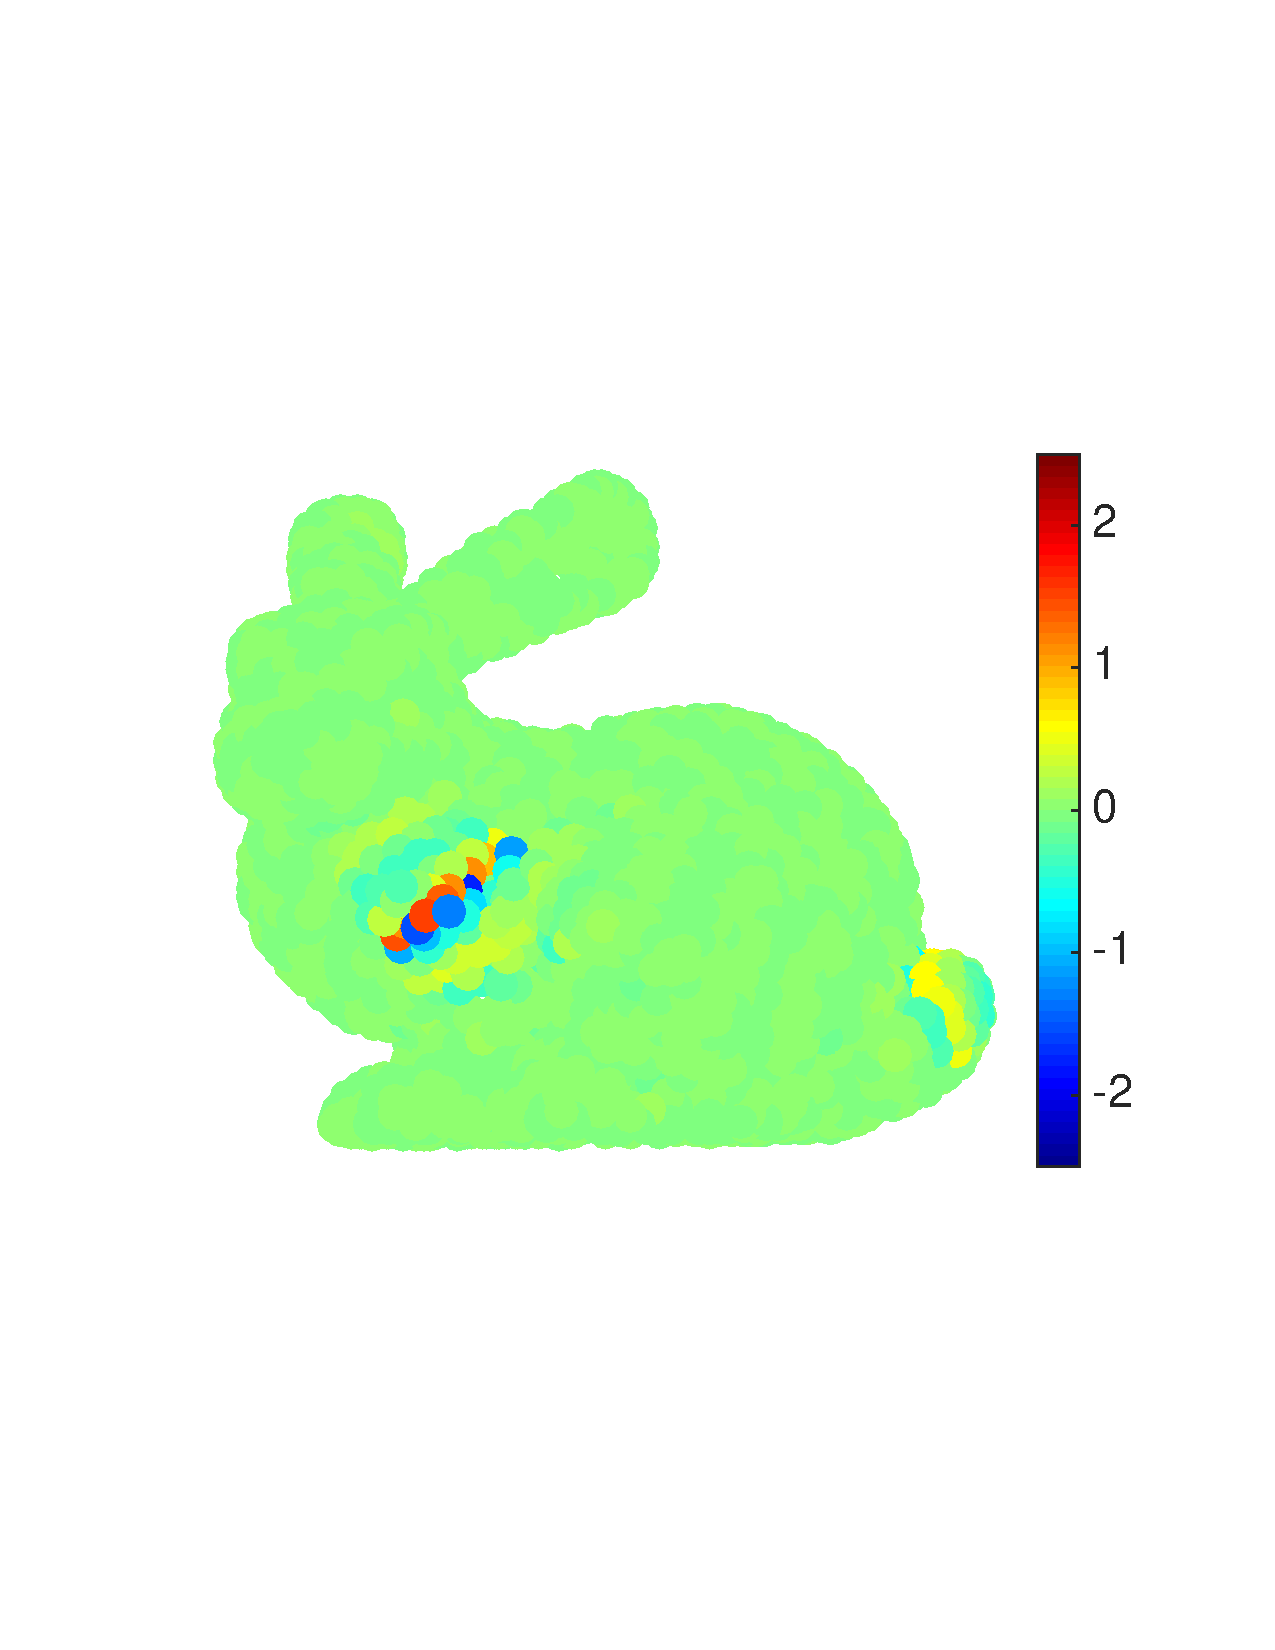
\includegraphics[width=.85\linewidth]{fig_bunny_rec_wav4}}
\end{minipage}
\caption{$M$-channel filter bank example. The first row shows example atoms in the vertex domain. The second row shows all atoms in the spectral domain, with an average of the atoms in each band shown by the thick black lines. The third row shows the analysis coefficients of Fig.\ \ref{Fig:bunny_signal}(d) by band, and the last row is the interpolation by band from those coefficients.}\label{Fig:bunny_coef}
\end{figure*}

\begin{figure}[tbh]
\begin{minipage}[m]{0.48\linewidth}
\centerline{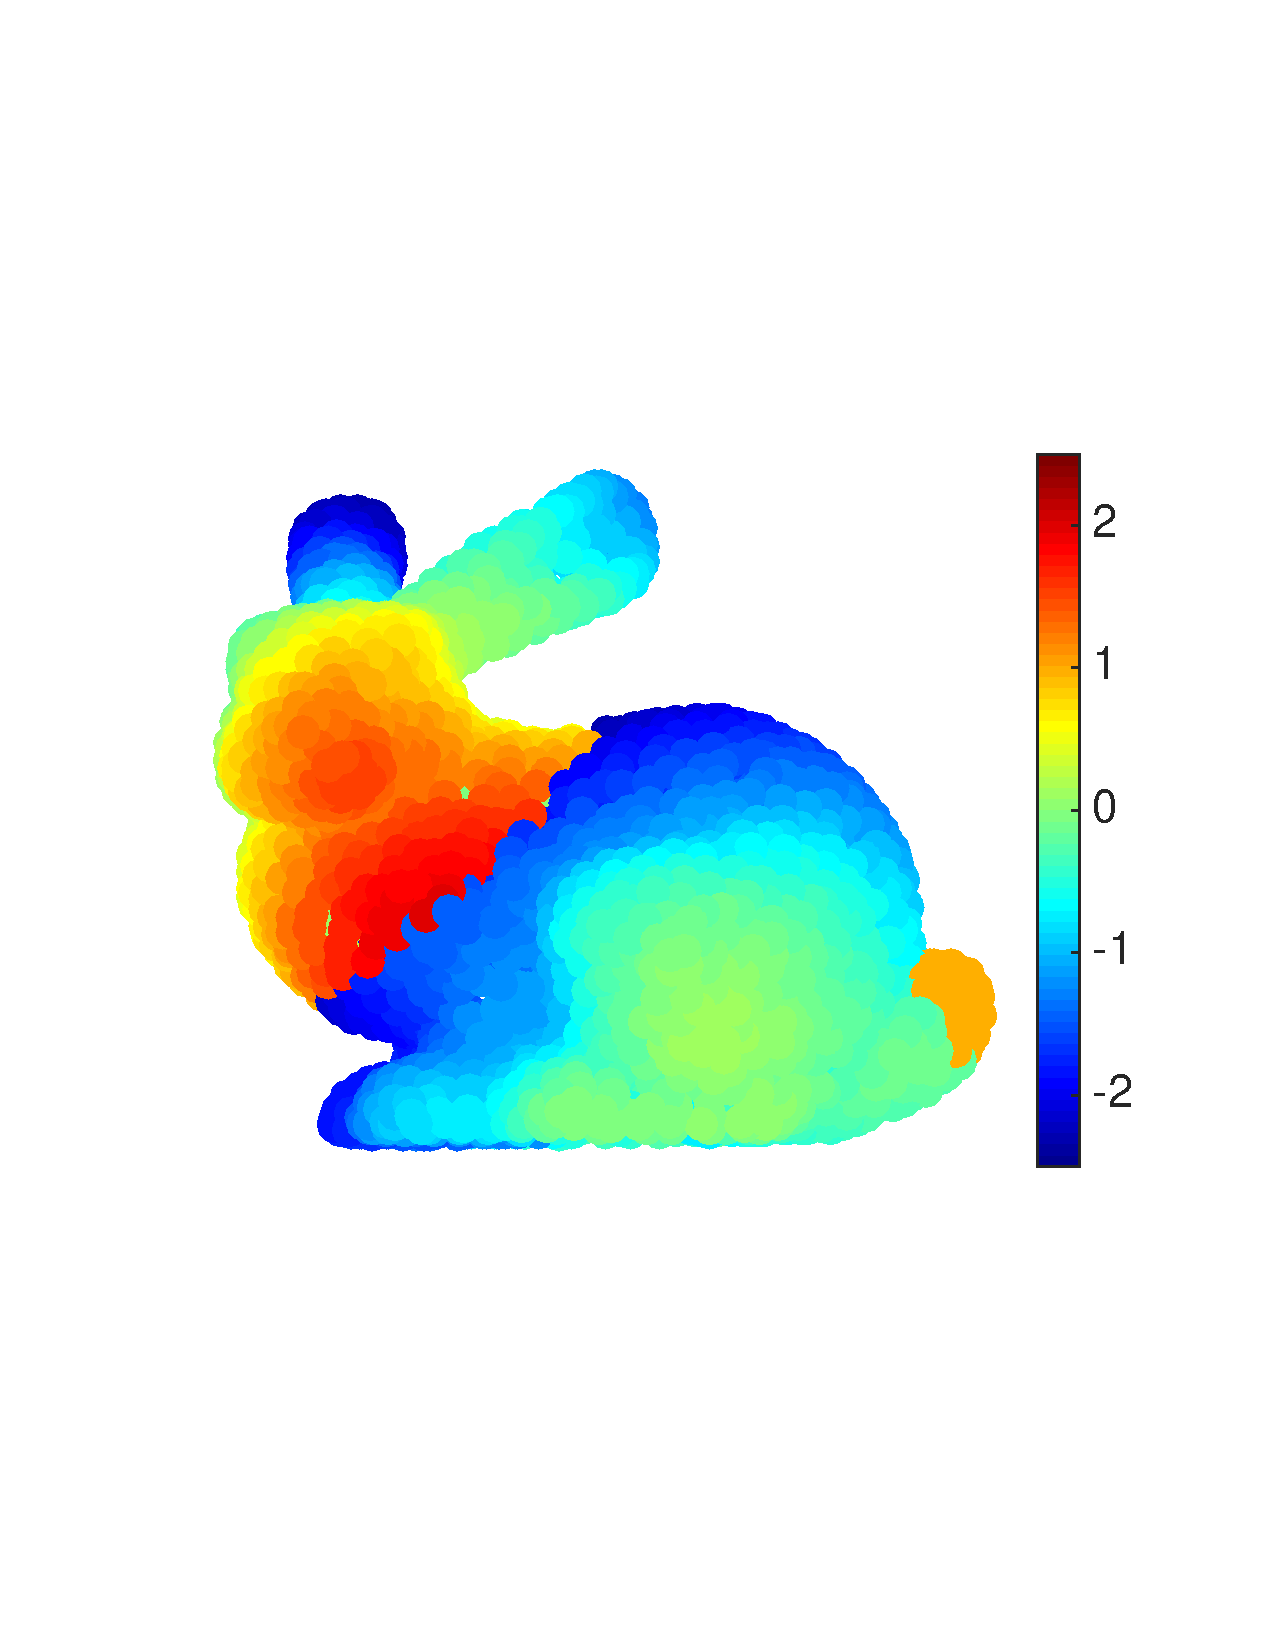
\includegraphics[width=.8\linewidth]{fig_bunny_signal}}
\centerline{\small{(a)}}
\end{minipage}
\begin{minipage}[m]{0.48\linewidth}
\centerline{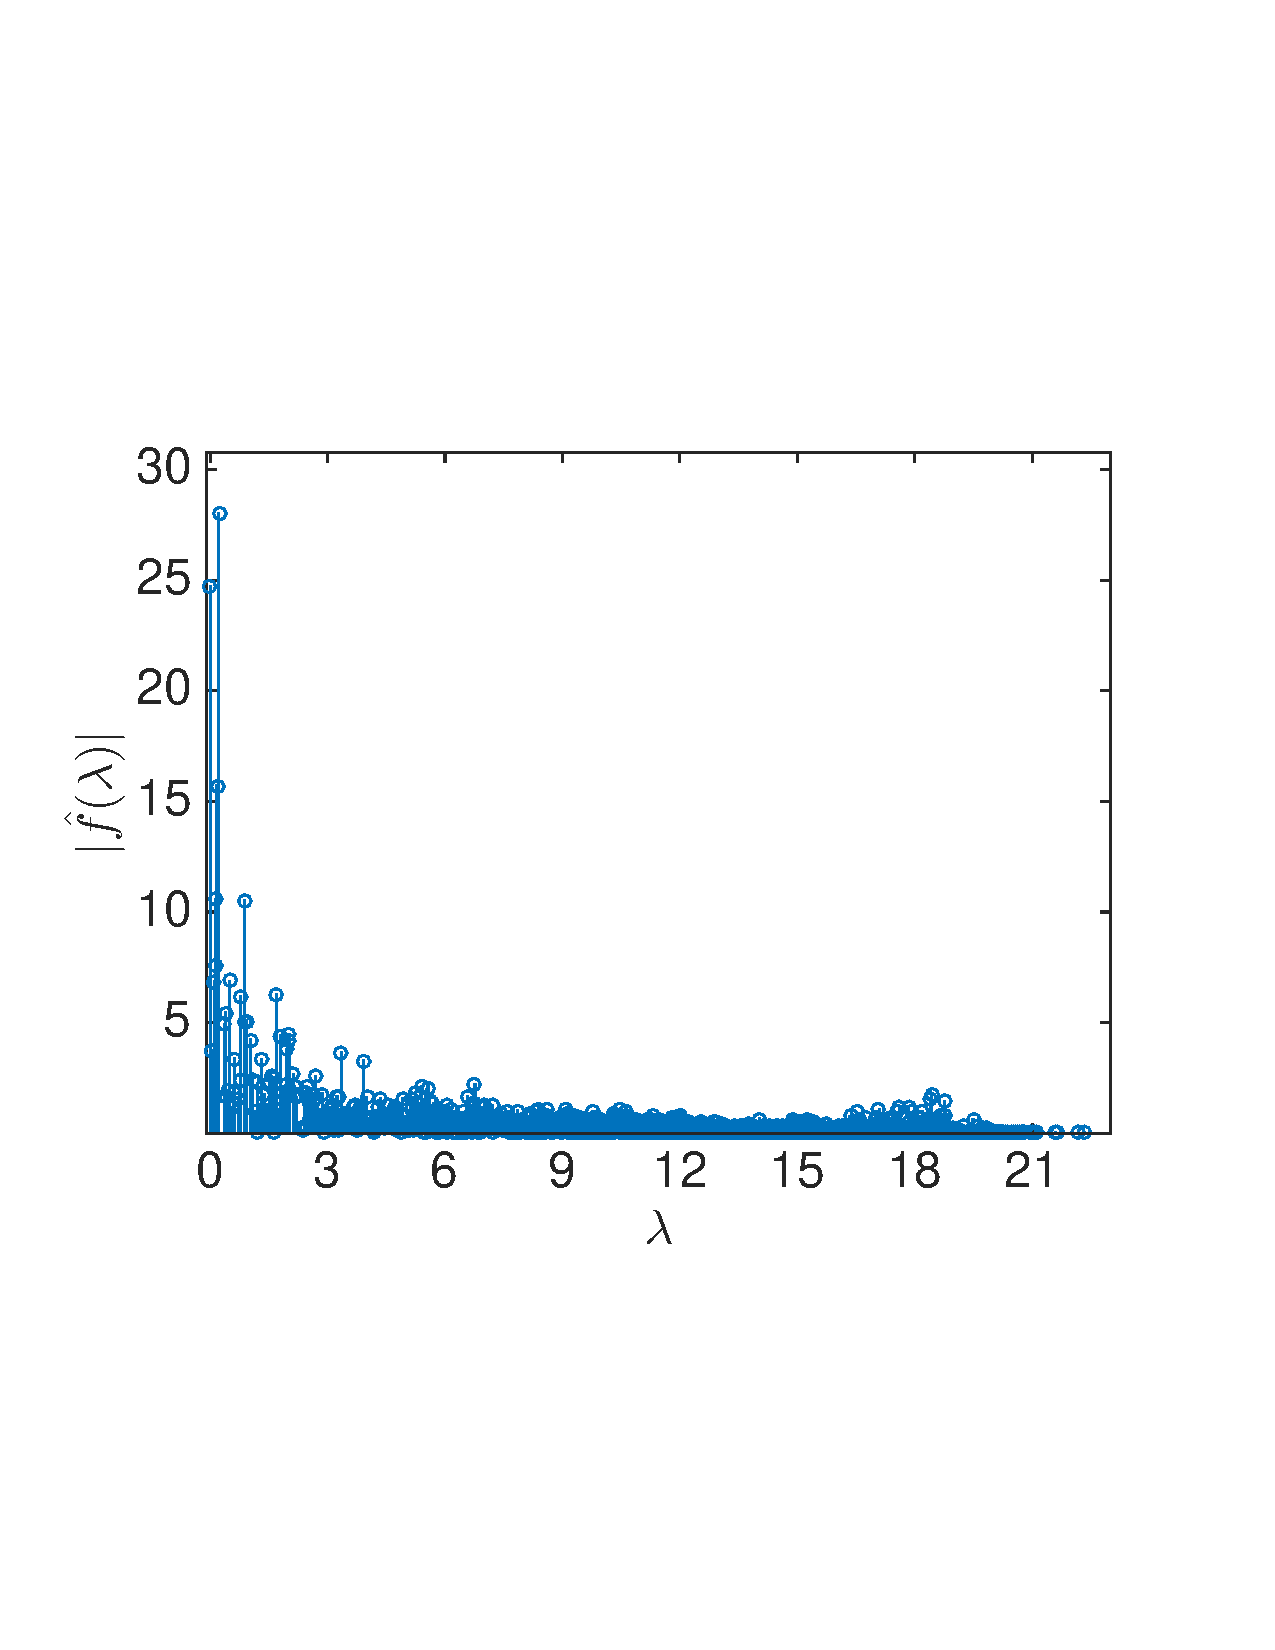
\includegraphics[width=.8\linewidth]{fig_bunny_signal_hat}~~~~~~~}
\centerline{\small{(b)}}
\end{minipage} \\
\begin{minipage}[m]{0.48\linewidth}
\centerline{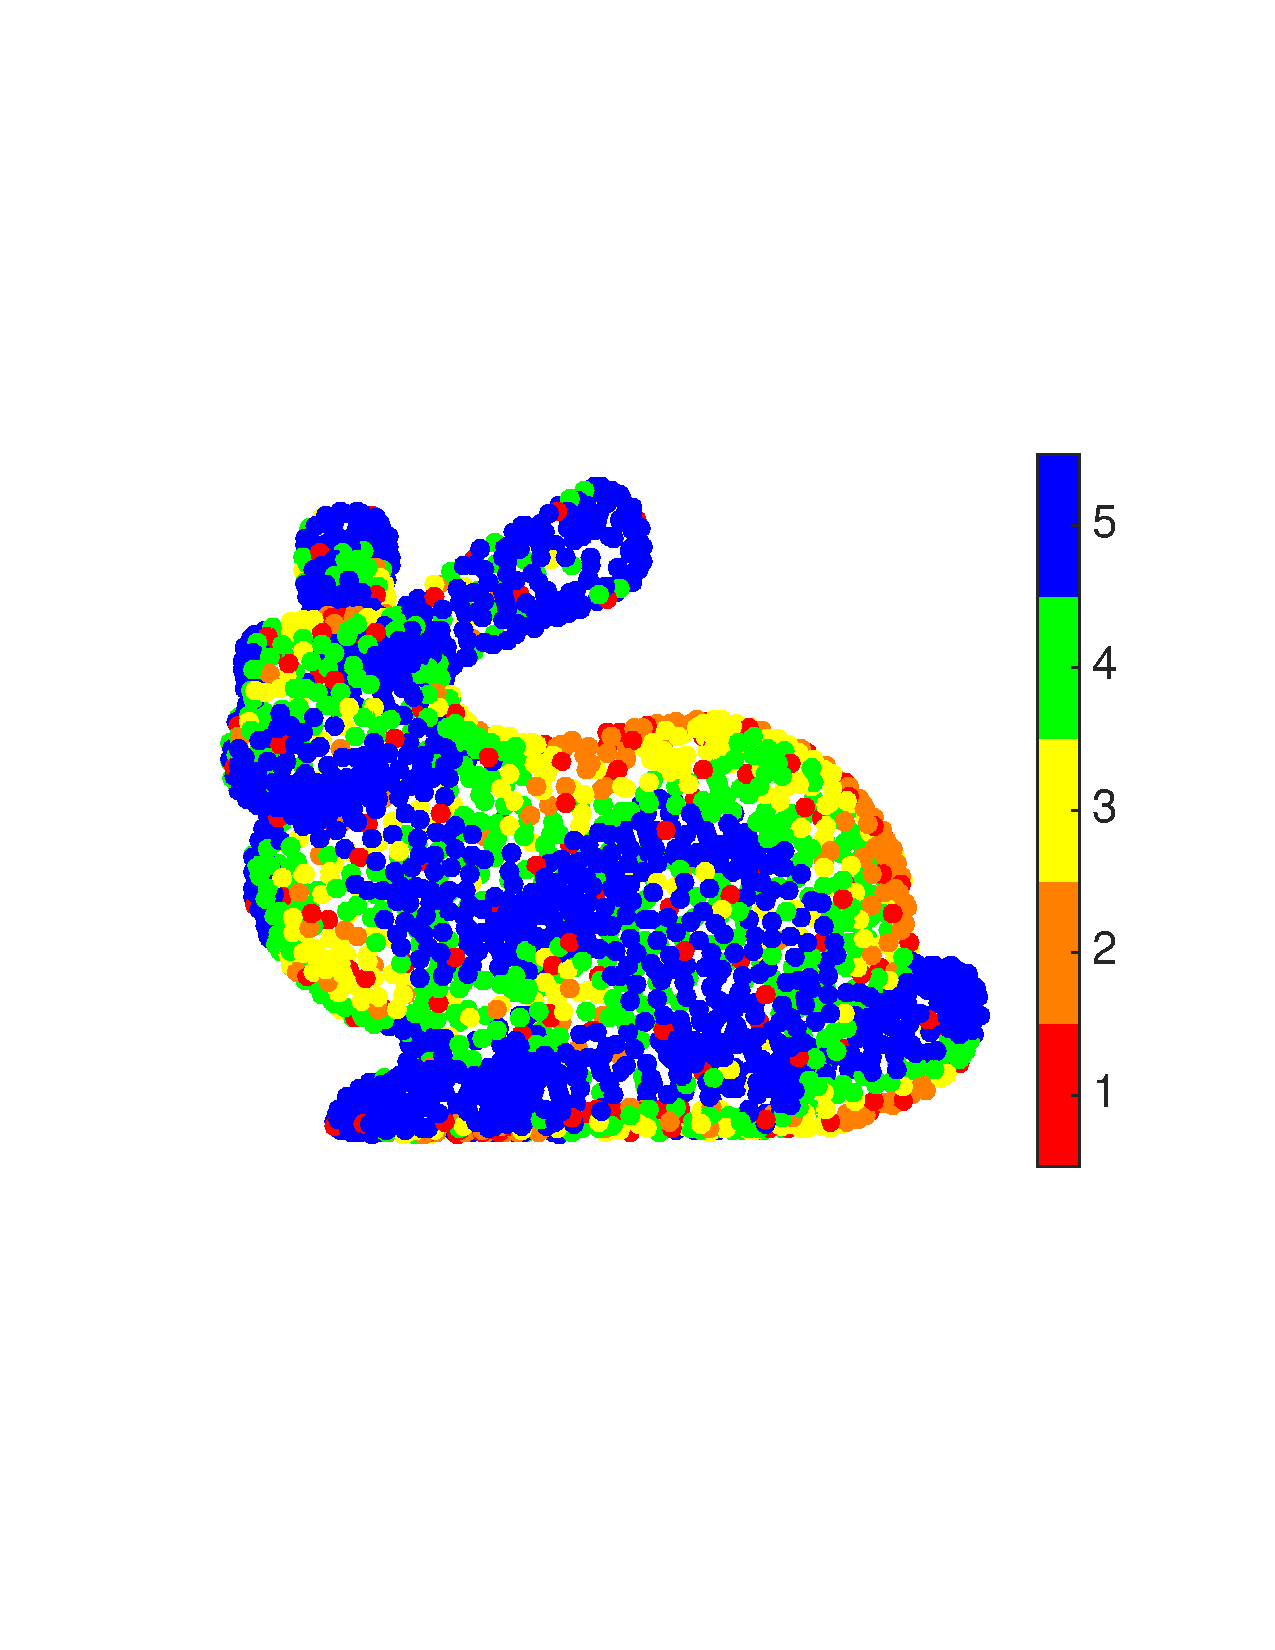
\includegraphics[width=.8\linewidth]{fig_bunny_partition}}
\centerline{\small{(c)}}
\end{minipage}
\begin{minipage}[m]{0.48\linewidth}
\centerline{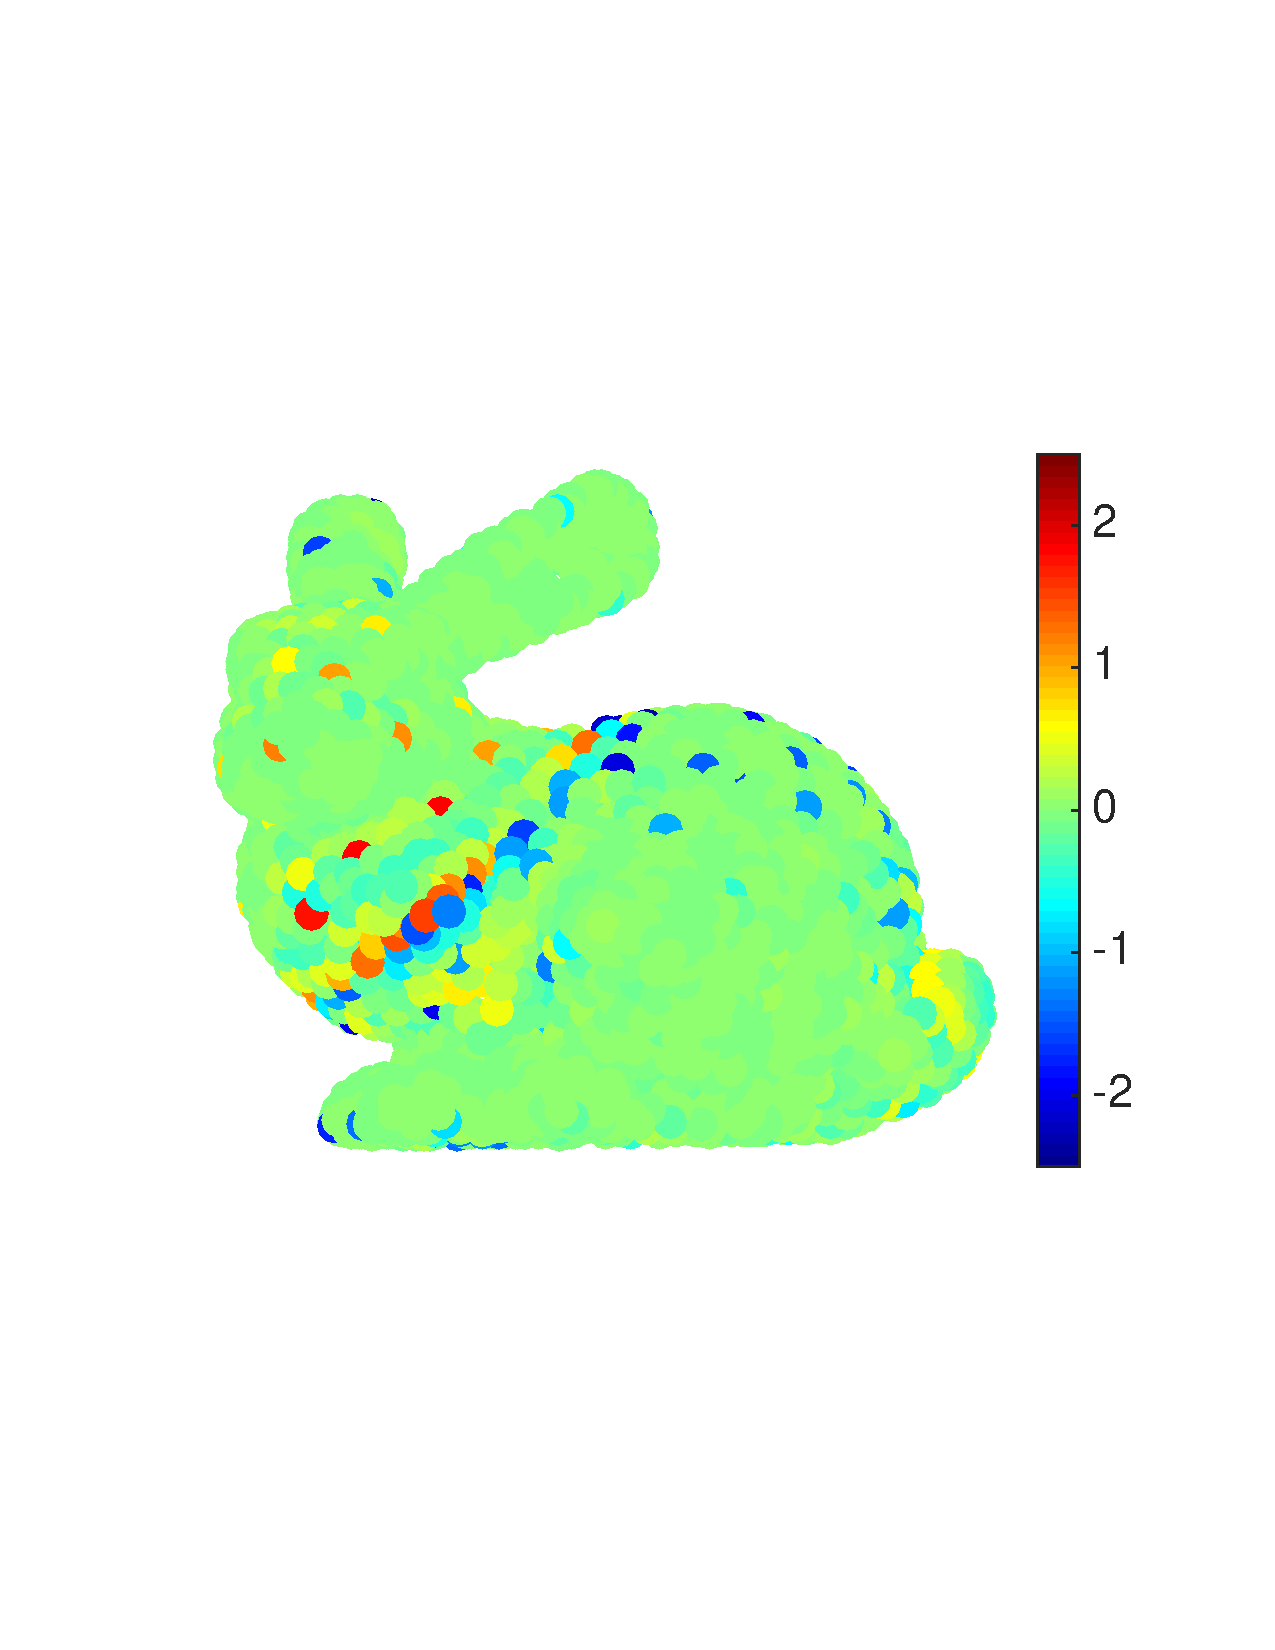
\includegraphics[width=.8\linewidth]{fig_bunny_coef_all}}
\centerline{\small{(d)}}
\end{minipage}
\caption{(a)-(b) Piecewise smooth signal on the Stanford bunny graph \cite{bunny} in the vertex and graph spectral domains, respectively. (c) Partition of the graph into uniqueness sets for five different spectral bands. (d) $M$-channel filter bank analysis coefficients of the signal shown in (a) and (b).}\label{Fig:bunny_signal}
\end{figure}

\subsection{Joint vertex-frequency localization of atoms and example analysis coefficients}
We start by empirically showing that the dictionary atoms (the columns of $\boldsymbol{\Phi}$) are jointly localized in the vertex and graph spectral domains. On the Stanford bunny graph \cite{bunny} with 2503 vertices, we partition the spectrum into five bands, and show the resulting partition into uniqueness sets 
in Fig.\ \ref{Fig:bunny_signal}(c). The first row of Fig.\ \ref{Fig:bunny_coef} shows five different example atoms whose energy is concentrated on different spectral bands. We see that these atoms are generally localized in the vertex domain as well. Some atoms such as the one shown at wavelet scale 3 are more spread in the vertex domain, possibly as a result of using ideal filters in the filter bank, an issue we revisit in Section \ref{Se:ill2}. The second row of Fig.\ \ref{Fig:bunny_coef} shows the spectral content of all atoms in each band, with the average for each represented by a thick black line. As expected, the energies of the atoms are localized in the spectral domain as well. 

Next we apply the proposed transform to a piecewise-smooth graph signal $f$ that is shown in the vertex domain in Fig.\ \ref{Fig:bunny_signal}(a), and in the graph spectral domain in Fig.\ \ref{Fig:bunny_signal}(b). The full set of analysis coefficients is shown in Fig.\ \ref{Fig:bunny_signal}(d), and these are separated by band in the third row of Fig.\ \ref{Fig:bunny_coef}. We see that with the exception of the lowpass channel, the coefficients are clustered around the two main discontinuities (around the midsection and tail of the bunny). The bottom row of Fig.\ \ref{Fig:bunny_coef} shows the interpolation of these coefficients onto the corresponding spectral bands, and if we sum these reconstructions together, we recover exactly the original signal in Fig.\ \ref{Fig:bunny_signal}(a).


\subsection{Sparse approximation}
Next, we compress 
a piecewise-smooth graph signal ${\bf f}$ via the sparse coding optimization
\begin{align}\label{Eq:sparse_coding}
\argmin_{\bf x}   || {\bf f}-\boldsymbol{\Phi}{\bf x} ||_2^2 \hbox{~~~subject to } ||{\bf x}||_0 \leq T,
\end{align}
where $T$ is a predefined sparsity level. After first normalizing the atoms of various critically-sampled dictionaries, we use the greedy %approximately solve the optimization problem
 % with 
 orthogonal matching pursuit (OMP) algorithm \cite{tropp2004greed,elad_book} to approximately solve \eqref{Eq:sparse_coding}. For the $M$-channel filter bank, the partition into uniqueness sets is shown in Fig. \ref{Fig:part_examples}, and the filter bank is shown in Fig. \ref{Fig:fb}. We show the reconstruction errors in Fig. \ref{Fig:comp}(d). 

\begin{figure}[tbh]
\begin{minipage}[m]{0.48\linewidth}
\centerline{~~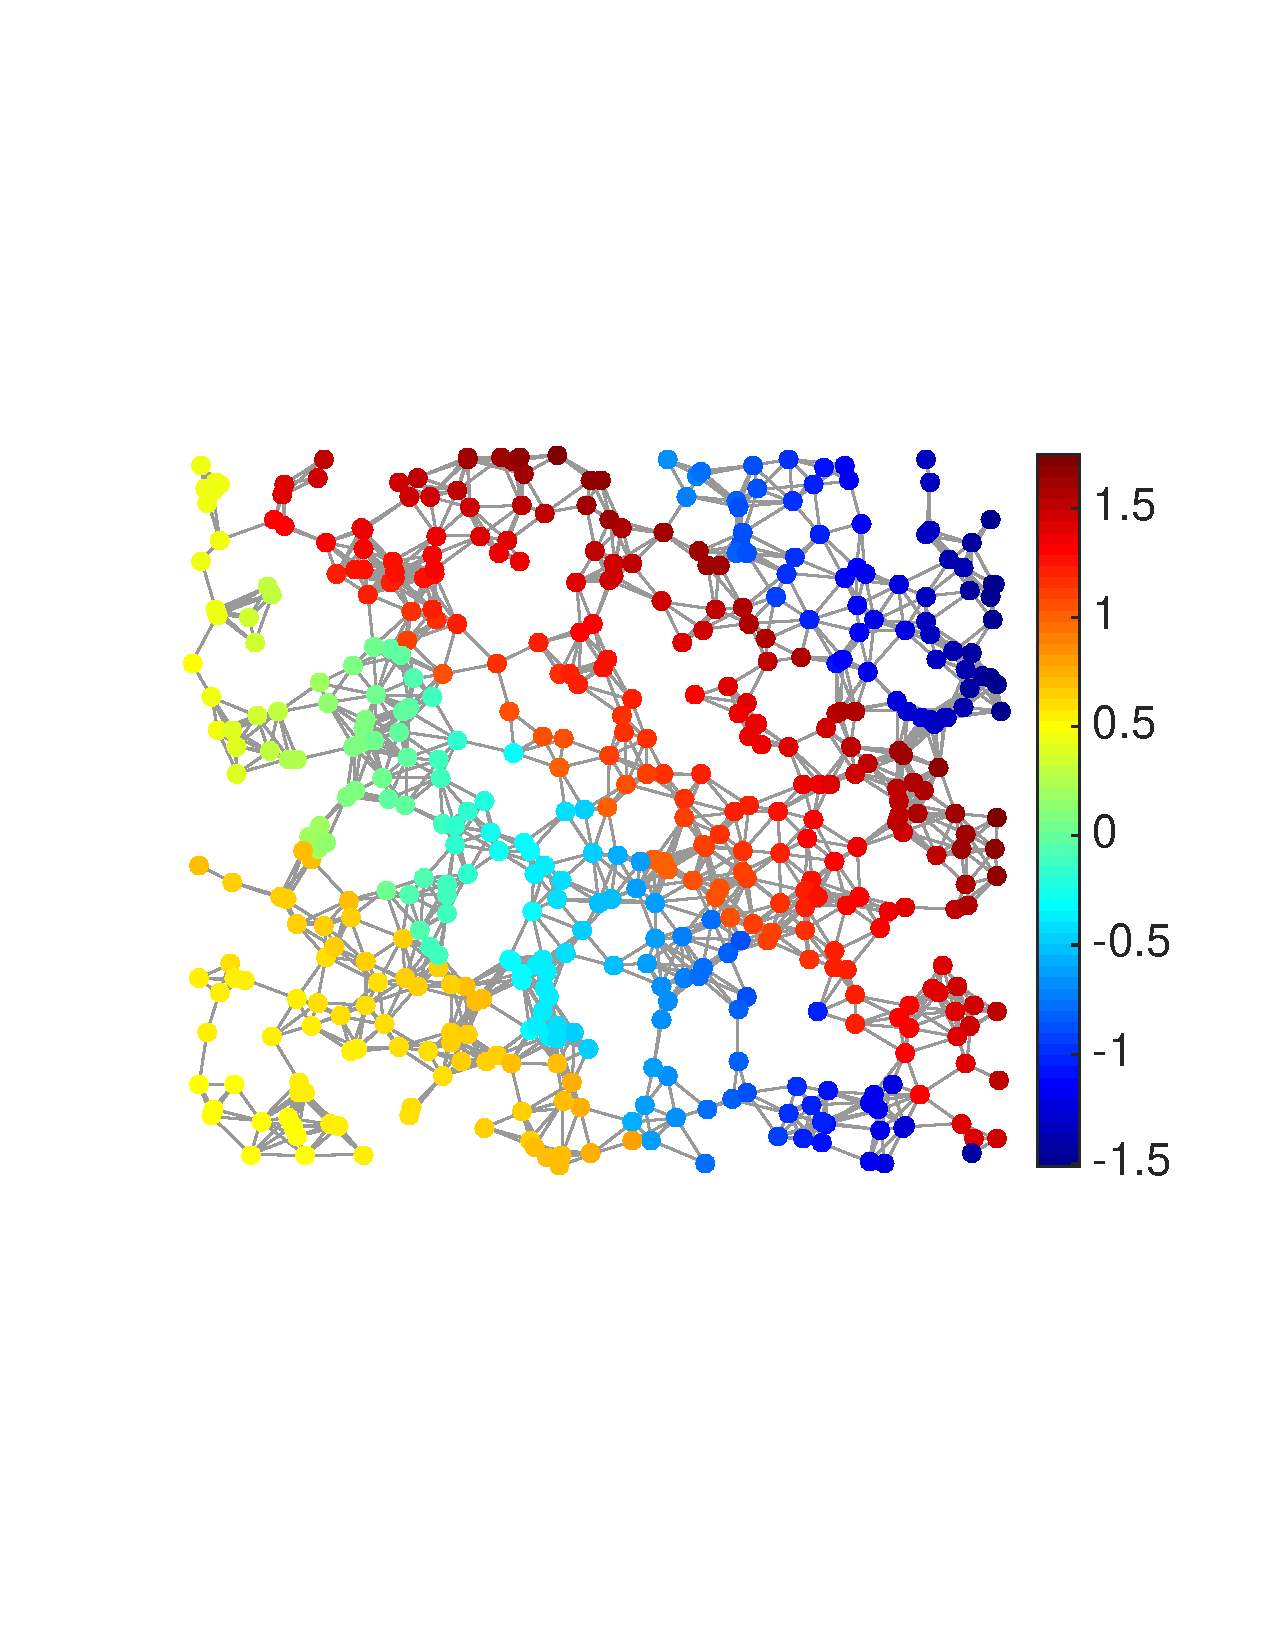
\includegraphics[width=.9\linewidth]{fig_comp_sig}}
\vspace{.05in}
\centerline{\small{(a)}}
\end{minipage}
\begin{minipage}[m]{0.48\linewidth}
\vspace{.02in}
\centerline{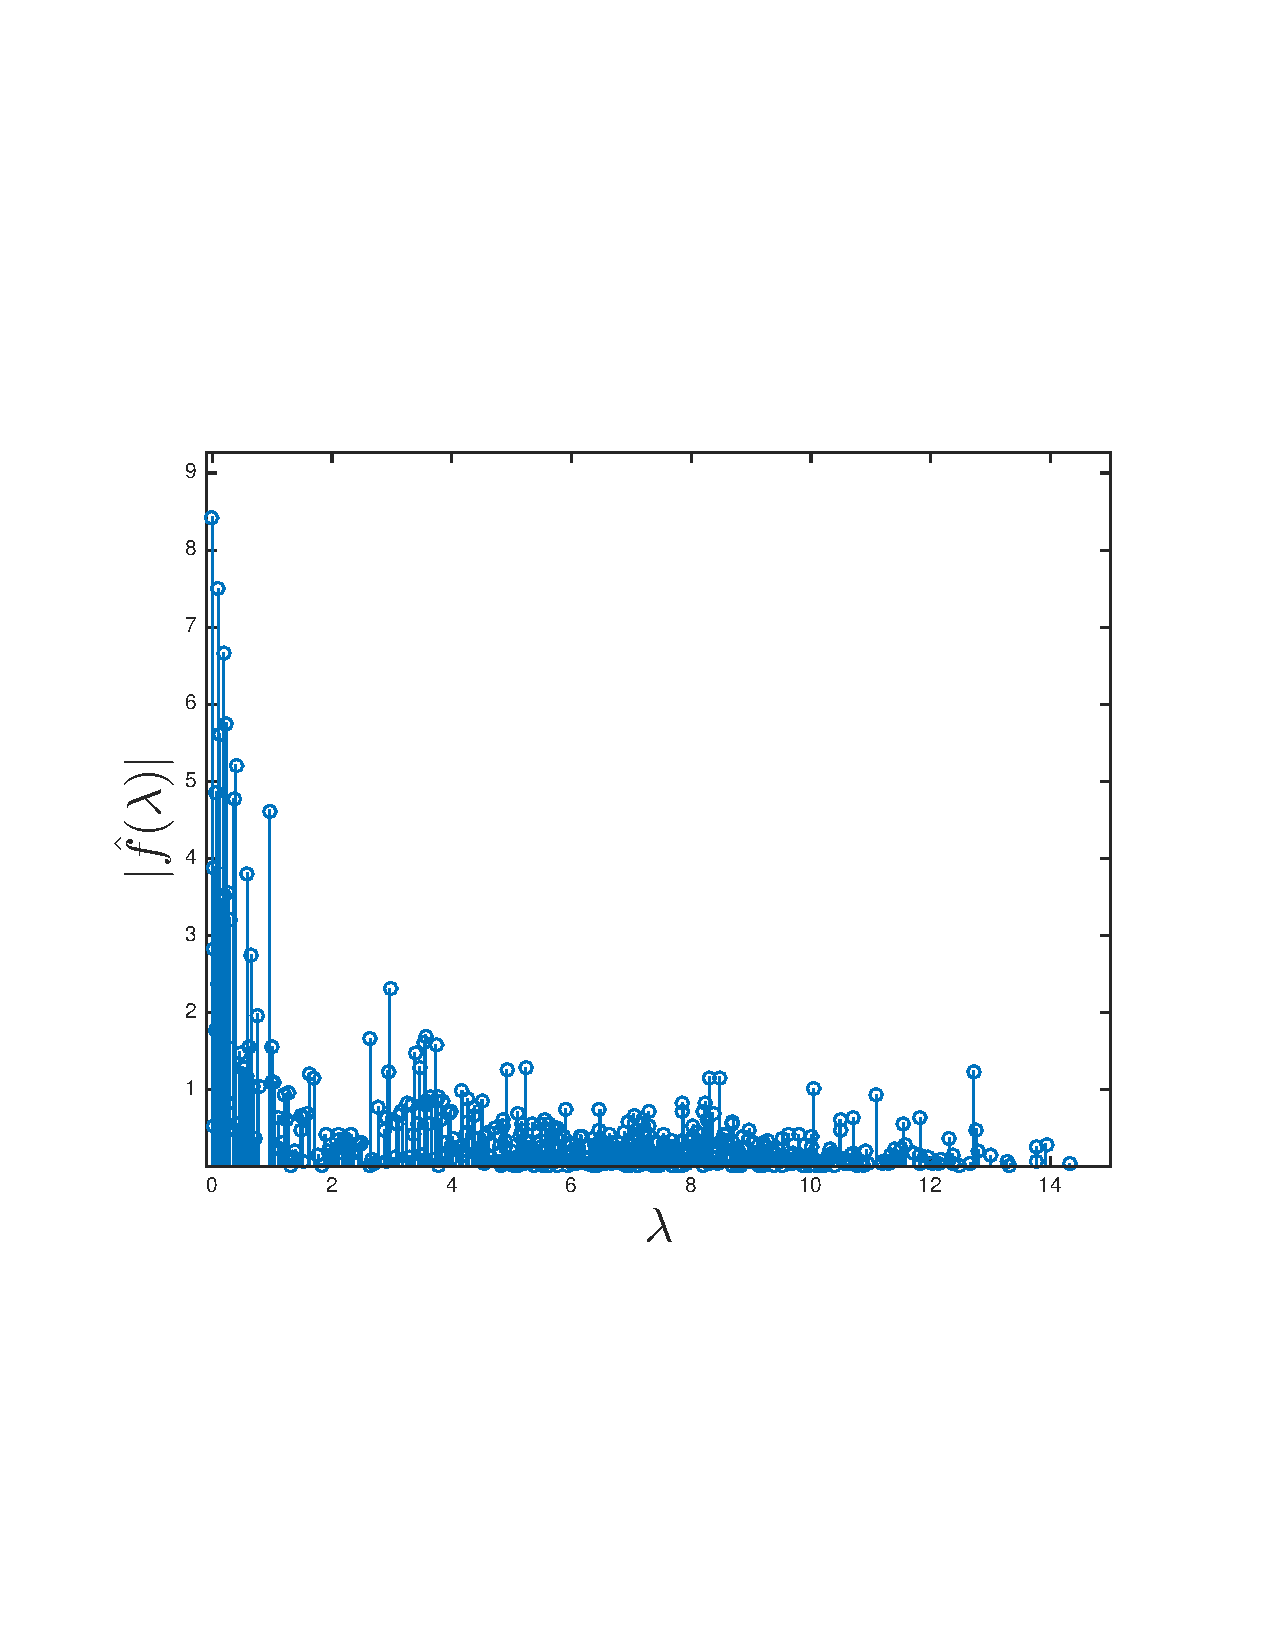
\includegraphics[width=.9\linewidth]{fig_comp_sig_hat}~}
\centerline{\small{(b)}}
\end{minipage} \\
\vspace{.07in}
\begin{minipage}[m]{0.48\linewidth}
\centerline{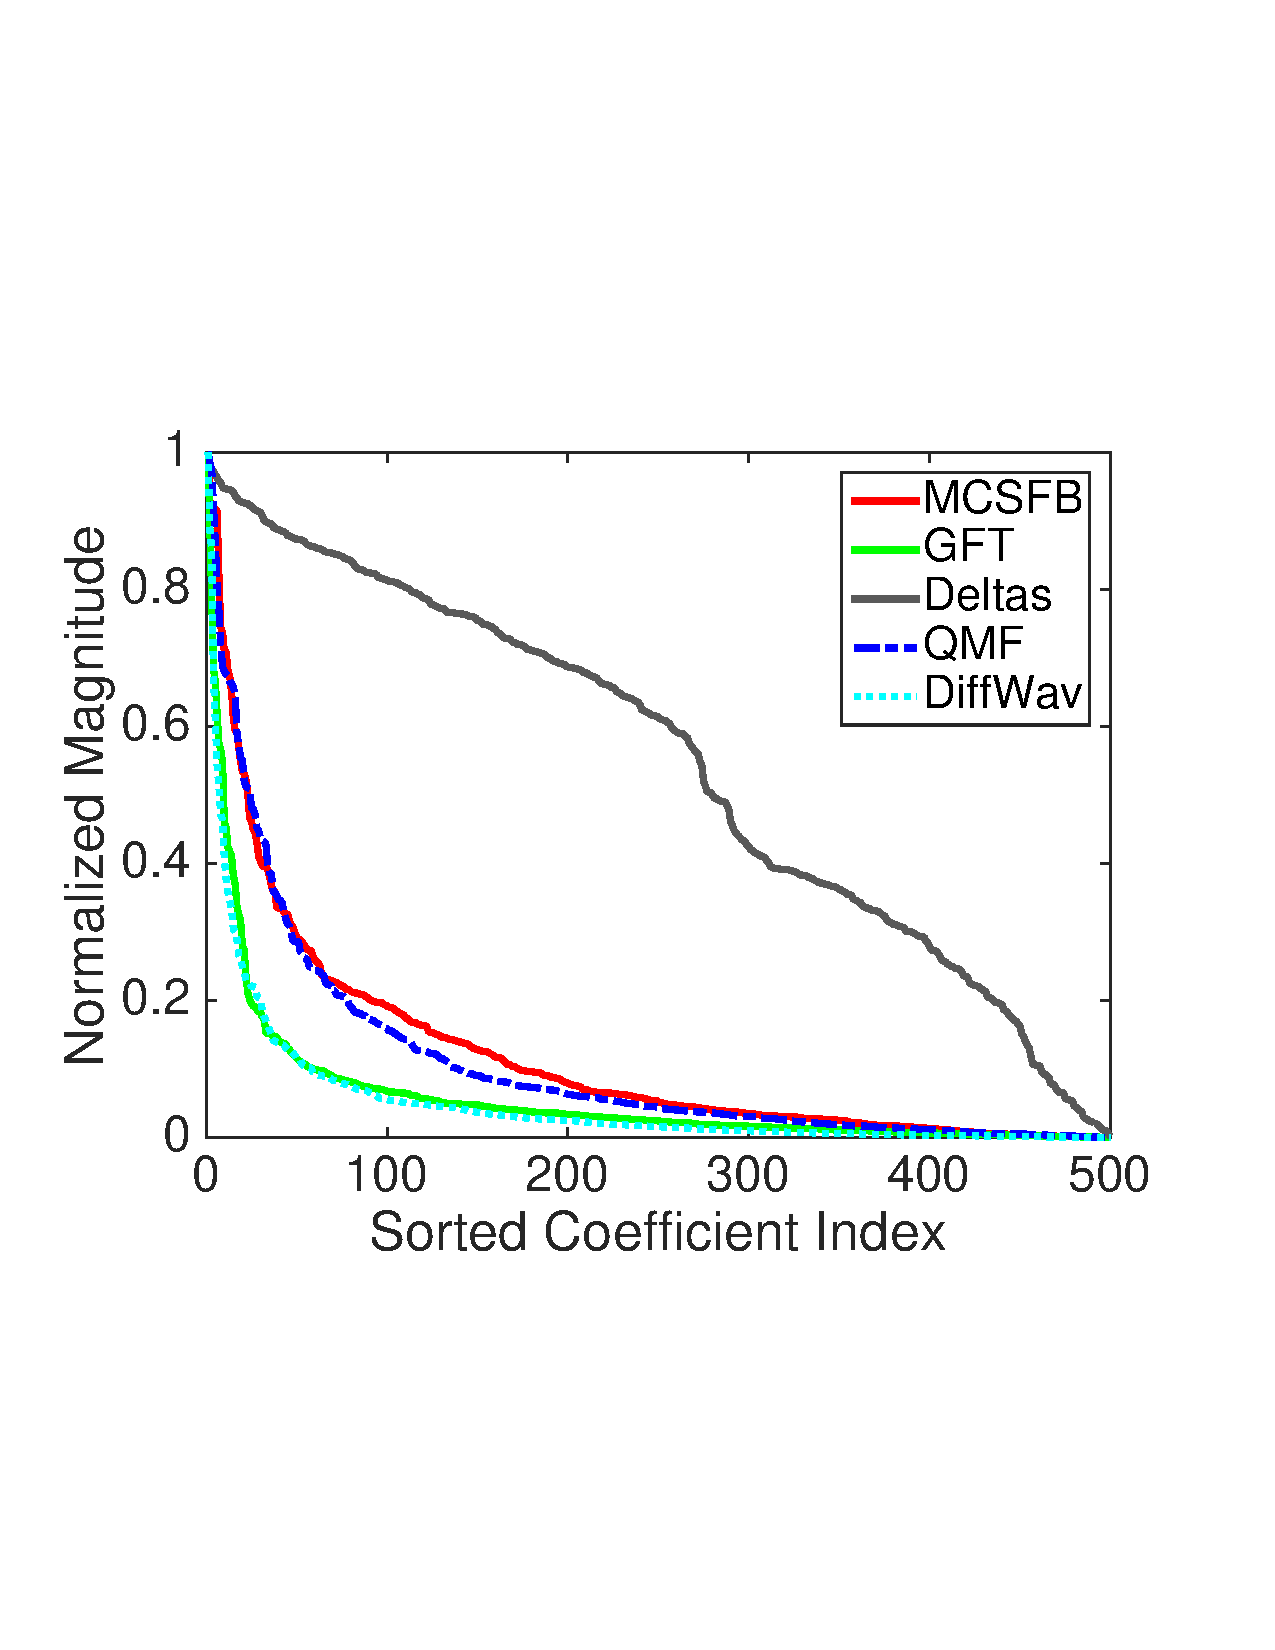
\includegraphics[width=.96\linewidth]{fig_comp_coeff2}}
\centerline{\small{(c)}}
\end{minipage}
\begin{minipage}[m]{0.48\linewidth}
\centerline{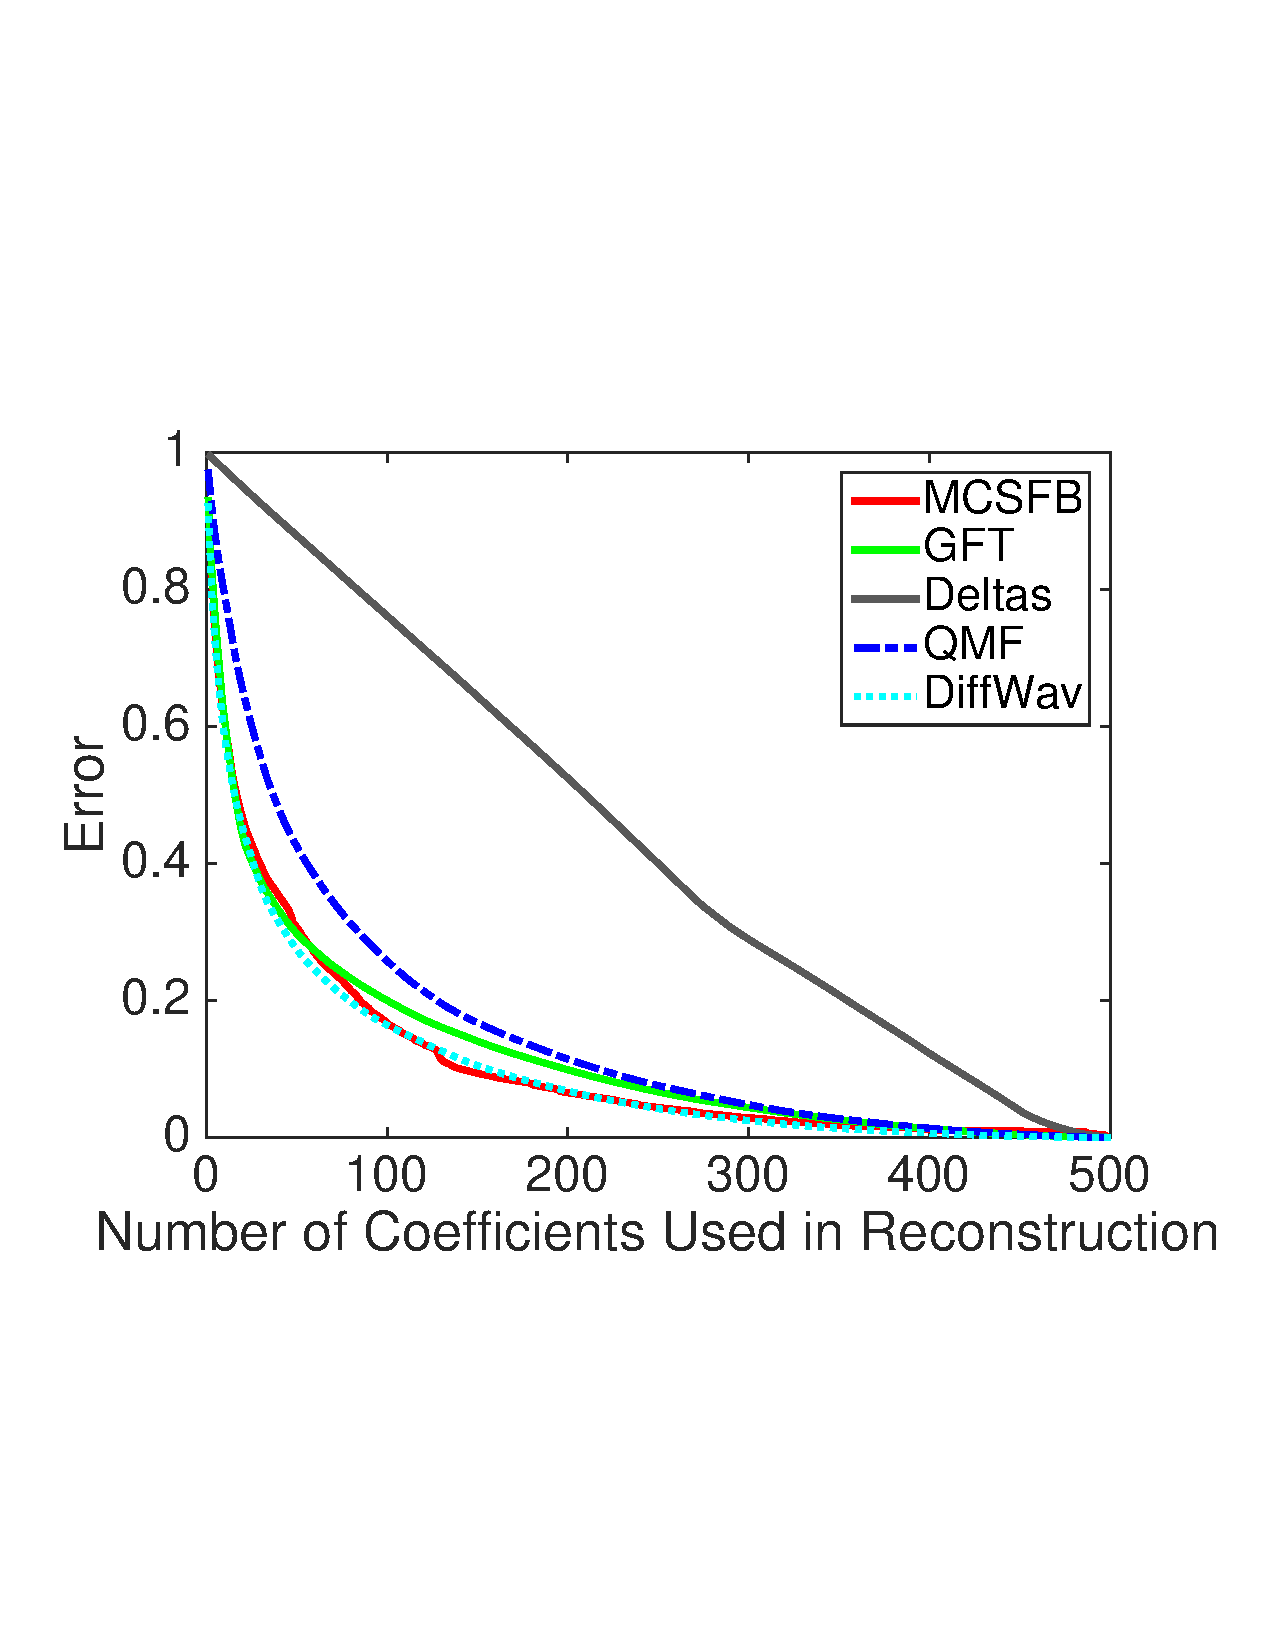
\includegraphics[width=.98\linewidth]{fig_comp_error}}
\centerline{\small{(d)}}
\end{minipage}
\caption{Compression example. (a)-(b) Piecewise-smooth signal from \cite[Fig. 11]{shuman_TSP_multiscale} in the vertex and graph spectral domains. (c) The normalized sorted magnitudes of the transform coefficients for the proposed $M$-channel critically sampled filter bank, the graph Fourier transform, the basis of Kronecker deltas, the quadrature mirror filterbank \cite{narang2012perfect}, and the diffusion wavelet transform \cite{coifman2006diffusion}. (d) The reconstruction errors  $\frac{\left|\left|{\bf f}_{\mbox{reconstruction}}-{\bf f}\right|\right|_2}{||{\bf f}||_2}$, as a function of the sparsity threshold $T$ in \eqref{Eq:sparse_coding}.} \label{Fig:comp}
\end{figure}


\section{Polynomial Filter Bank Design}
In the numerical examples in the previous sections, we have computed a full eigendecomposition of the graph Laplacian and subsequently used it for all three of the filtering, sampling, and interpolation operations; however, such an eigendecomposition does not scale well with the size of the graph as it requires ${\cal O}(N^3)$ operations with naive methods. In these next three sections, we develop a fast approximate version of the proposed transform that scales more efficiently for large, sparse graphs. 

\subsection{Approximation by polynomial filters} \label{Se:poly_approx}

Fast, approximate methods for computing $h_m(\L){\bf f}$ a function of sparse matrix times a vector, include approximating the function $h_m(\cdot)$ by a polynomial (e.g., via a truncated Chebyshev or Legendre expansion), approximating $h_m(\cdot)$ by a rational function, Krylov space methods (Lanczos in our case of a symmetric matrix $\L$), the matrix version of the Cauchy integral theorem (see, e.g., \cite{higham}\nocite{davies2005computing, frommer}-\cite{dubious} and references therein). The first three of these methods have been examined in graph signal processing settings \cite{hammond2011wavelets,PuyTGV15},  \cite{shuman_distributed_sipn}\nocite{susnjara, shi2015infinite}-\cite{loukas2015distributed}. While all of these could be used to approximate the filters in the analysis step of the proposed filter bank, we focus on order $K$ Chebyshev polynomial approximations of the form
\begin{align}\label{Eq:cheb}
\tilde{h}(\L){\bf f} := \sum_{k=0}^K \alpha_k \bar{T}_k(\L){\bf f}.
\end{align}
In \eqref{Eq:cheb}, $\bar{T}_k(\cdot)$ are Chebyshev polynomials shifted to the interval $[0,\lambda_{\max}]$. Thus,  $\bar{T}_0(\L){\bf f} = {\bf f}$, $\bar{T}_1(\L){\bf f} = \frac{2}{\lambda_{\max}}\L{\bf f}-{\bf f}$, and for $k\geq 2$, by the three term recurrence relation of Chebyshev polynomials, we have
\begin{align*}
\bar{T}_k(\L){\bf f} = \frac{4}{\lambda_{\max}}\left(\L-\frac{\lambda_{\max}}{2}{\bf I}\right)\bar{T}_{k-1}(\L){\bf f}-\bar{T}_{k-2}(\L){\bf f}.
\end{align*}


%{\color{blue}
The coefficients in \eqref{Eq:cheb} are often taken to be $\alpha_0=\frac{1}{2}c_0$ and $\alpha_k=c_k$ for $k=1,2,\ldots,K$, where  $\{c_k\}_{k=0,\ldots,K}$ are the truncated Chebyshev expansion coefficients 
%\cite{jay} formula
\begin{align*}
c_{k}&:=\langle h , \bar{T}_k \rangle \\&~= \frac{2}{\pi}\int_{0}^{\pi}\cos(k\phi)~h\Bigl(\frac{\lambda_{\max}}{2} \bigl(\cos(\phi) +1\bigr)\Bigr)~d\phi.
\end{align*}
However, the oscillations that arise in Chebyshev polynomial approximations of bandpass filters may result in larger values of $\tilde{h}_m(\lambda)\tilde{h}_{m^{\prime}}(\lambda)$, even when the ideal filters $h_m(\cdot)$ and $h_{m^{\prime}}(\cdot)$ have supports that do not come close to overlapping. This negates the orthogonality of the atoms across bands shown in \eqref{Eq:ortho_bands}. In an attempt to at least preserve \emph{near} orthogonality across bands, we 
% Note that if 
%\begin{itemize}
%%\item $c_k$ formula for truncated Chebyshev expansion
%\item However
%%\item To compute $g_i(\L)f$, Matrix function times a vector literature (2-3 general surveys, graph signal processing literature) the polynomial approximation method discussed in \cite{hammond2011wavelets,shuman_DCOSS_2011}
%%\item Approximate filtering, and theory showing that the error (i) clusters around boundaries, and (ii) only matters where there are eigenvalues, approximation error
%\item Use Jackson-Chebyshev, in attempt to preserve orthogonality across bands. Give equations, references, and explain damping
%%\item Another advantage of the approximation is that the value of the filtered signal at a given vertex is a weighted average of the signal values in a neighborhood around that vertex \cite{shuman2013emerging}. 
%\end{itemize}
%}
therefore use the Jackson-Chebyshev polynomial approximations from \cite{di2016efficient,puy_structured_sampling} that damp the Gibbs oscillations appearing in Chebyshev expansions. With the damping, $\alpha_0=\frac{1}{2}c_0$ and $\alpha_k=\gamma_{k,K}c_k$ for $k=1,2,\ldots,K$, where, as presented in \cite{di2016efficient}, 
\begin{align*}
\gamma_{k,K} &= \frac{\left(1-\frac{k}{K+2}\right)\sin\left(\frac{\pi}{K+2}\right)\cos\left(\frac{k\pi}{K+2}\right)}{\sin\left(\frac{\pi}{K+2}\right)} \\
&~~~~+~\frac{\frac{1}{K+2}\cos\left(\frac{\pi}{K+2}\right)\sin\left(\frac{k\pi}{K+2}\right)}{\sin\left(\frac{\pi}{K+2}\right)}.
\end{align*}
%{\color{blue} Reference 
Figure \ref{Fig:approx_filtering_error} shows the Jackson-Chebyshev polynomial approximations for ideal bandpass filters of two different graphs.\footnote{For the net25 graph, we have removed the self loops and added a single edge to connect the two connected components.}

%}
\begin{figure}[tbh]
\begin{minipage}[m]{0.49\linewidth}
\centerline{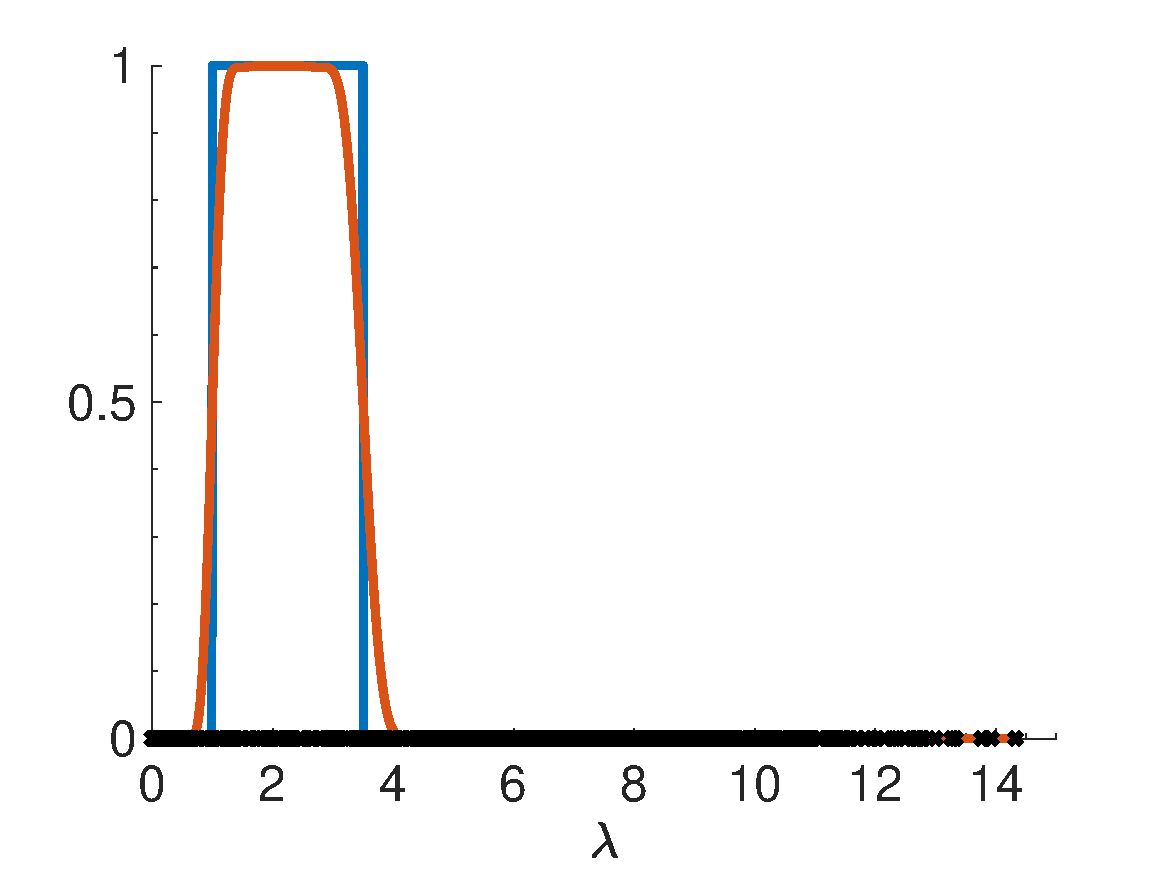
\includegraphics[width=1.1\linewidth]{fig_approx_filter_sensor}}
\centerline{~~\small{(a)}}
\end{minipage}
\begin{minipage}[m]{0.49\linewidth}
\centerline{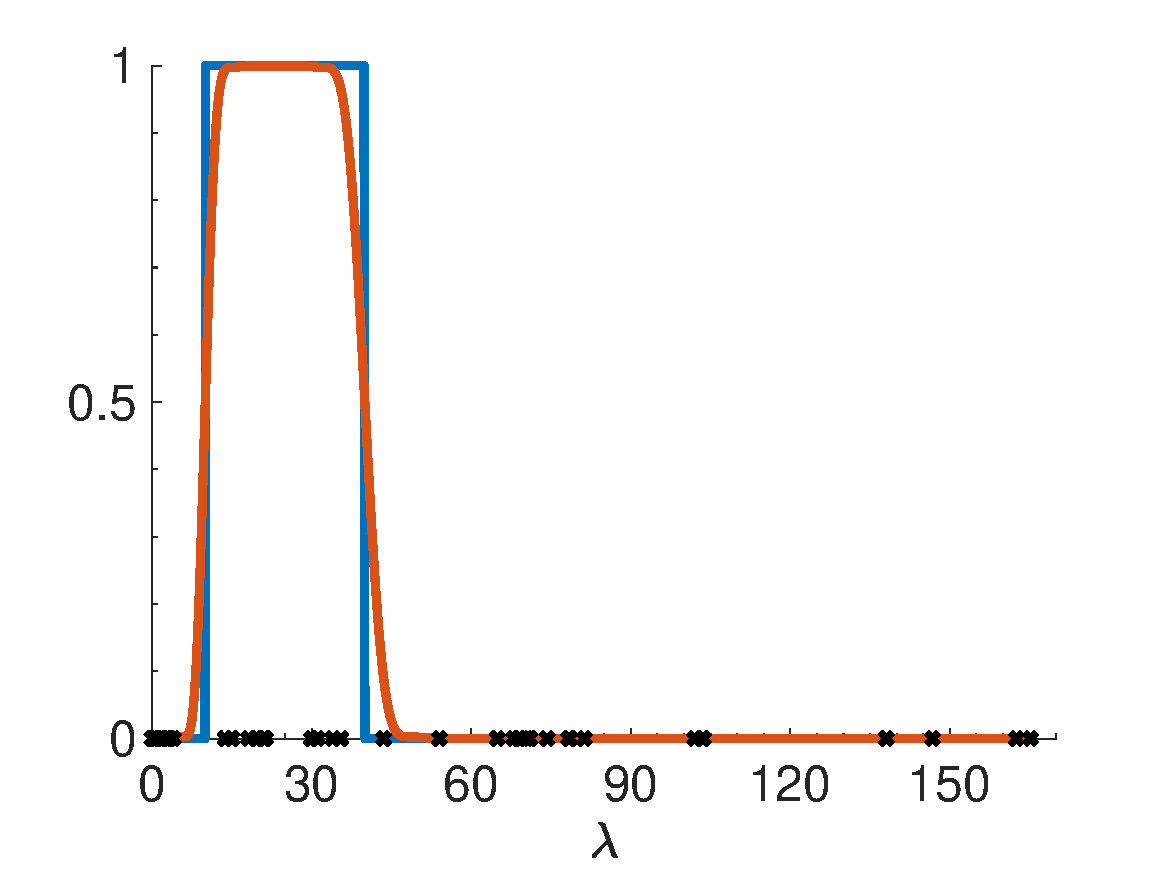
\includegraphics[width=1.1\linewidth]{fig_approx_filter_net25}}
\centerline{~~\small{(b)}}
\end{minipage} \\
\begin{minipage}[m]{0.49\linewidth}
\centerline{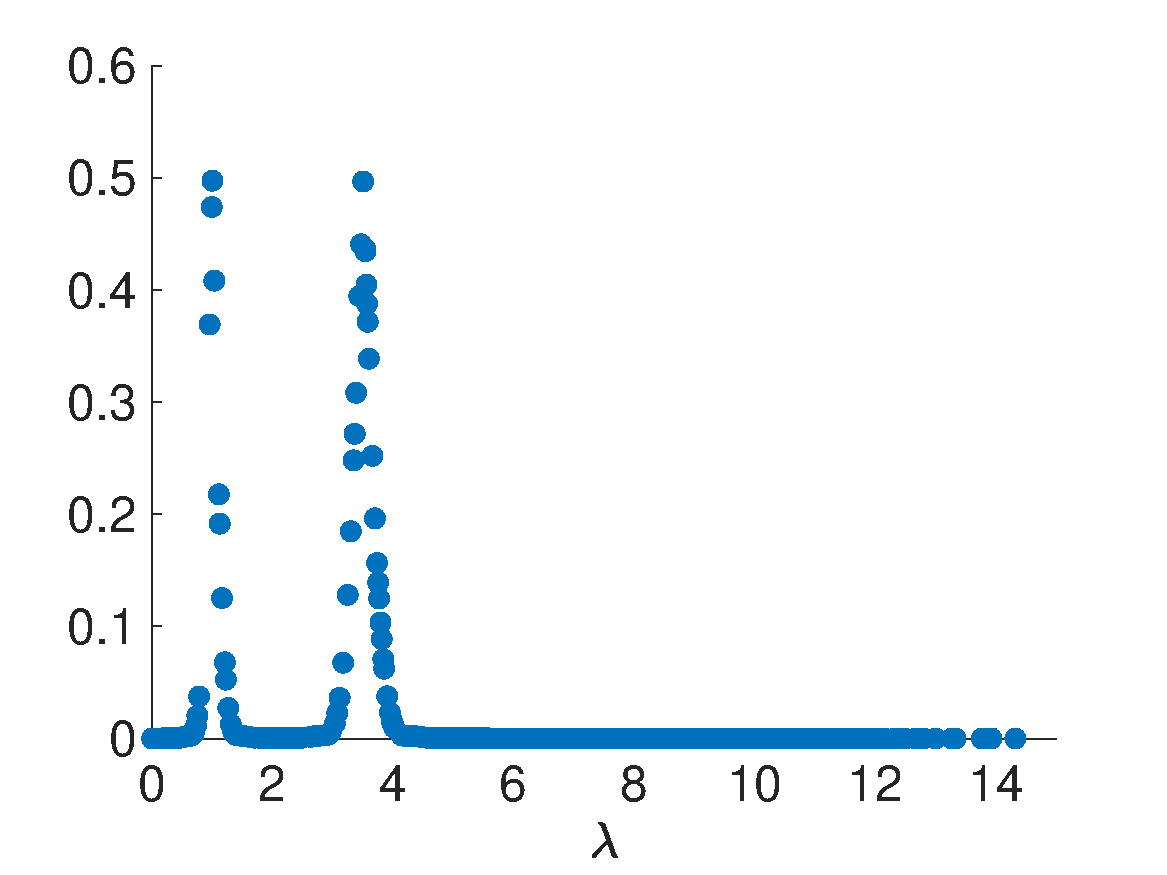
\includegraphics[width=1.1\linewidth]{fig_approx_filter_sensor_error}}
\centerline{~~\small{(c)}}
\end{minipage}
\begin{minipage}[m]{0.49\linewidth}
\centerline{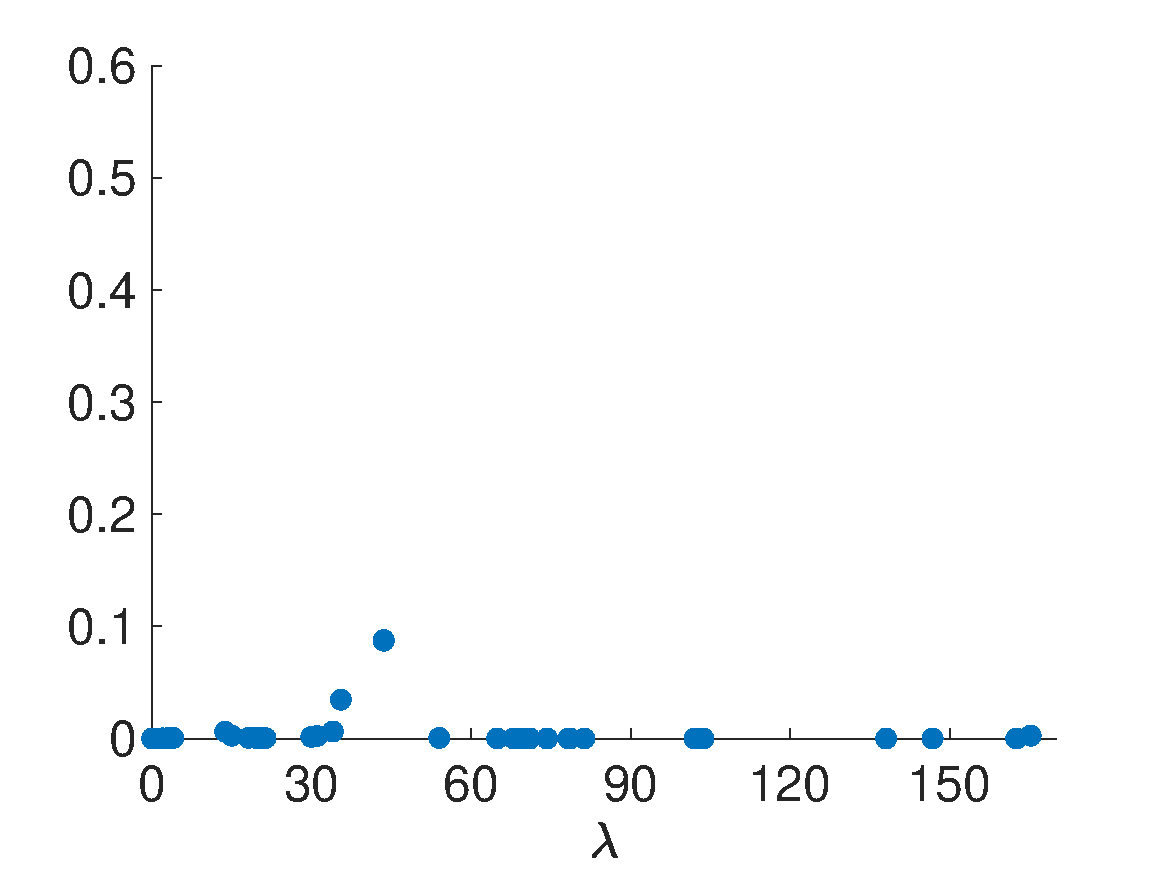
\includegraphics[width=1.1\linewidth]{fig_approx_filter_net25_error}}
\centerline{~~\small{(d)}}
\end{minipage}
\caption{Degree 80 Jackson-Chebyshev polynomial approximations for ideal bandpass filters on the (a) 500 vertex random sensor network of Figure \ref{Fig:part_examples} and (b) Andrianov net25 graph from \cite{davis2011university} with 9,520 vertices. In (c) and (d), we show the errors $|\tilde{h}(\lambda_{\l})-h(\lambda_{\l})|$ at each of the Laplacian eigenvalues of the corresponding graphs in (a) and (b).}
%\caption{{\color{red} Fix: check symmetry of second one, make the relative widths the same, show scatter plots of errors at eigenvalues, add Chebyshev?}
\label{Fig:approx_filtering_error}
\end{figure}

%{\protect\footnotemark} 
%\footnotetext{We have removed the self loops in the graph and added a single edge to connect the two connected components.}

\subsection{Filter bank design}

We can quantify the worst case error introduced when approximating  $h_m(\cdot)$ by an approximant $\tilde{h}_m(\cdot)$ as follows:
\begin{align} \label{Eq:poly_approx_error}
&||\tilde{h}_m(\L)-h_m(\L) ||_2  \nonumber \\ &~~~~~~~= \max_{\l \in \{0,1,\ldots,N-1\}}|\tilde{h}_m(\lambda_{\l})-h_m(\lambda_{\l}) |  \nonumber \\
 &~~~~~~~\leq \max_{\lambda \in [0,\lambda_{\max}]}|\tilde{h}_m(\lambda)-h_m(\lambda) |.
\end{align}
While approximation theory often aims to minimize the upper bound in \eqref{Eq:poly_approx_error}, only the errors exactly at the graph Laplacian eigenvalues affect the overall approximation error $||\tilde{h}_m(\L)-h_m(\L) ||_2$. Since, as seen in Figure \ref{Fig:approx_filtering_error}, the errors of the Jackson-Chebyshev polynomial approximation are concentrated around the discontinuities of $h_m(\cdot)$, a guiding principle when designing the filter bank to be more amenable to fast approximation is to choose the endpoints $\{\tau_m\}_{m=1,\ldots,M-1}$ of the bandpass filters to be in gaps in the graph Laplacian spectrum. Unfortunately, we do not have access to the exact graph Laplacian eigenvalues (the reason for introducing this approximation in the first place is that they are too expensive to compute for large graphs); however, we can efficiently estimate the density of the spectrum in order to design the filters in a way that aims to have the endpoints close to fewer eigenvalues of $\L$.

\subsubsection{Estimating the spectral density} \label{Se:spectral_density}

Lin et al. \cite{lin_spectral_density} provide an excellent overview of methods to approximate the \emph{spectral density function} \cite[Chapter 6]{van_mieghem}) (also called the \emph{Density of States} or \emph{empirical spectral distribution} \cite[Chapter 2.4]{tao_random_matrix}) of a matrix, which in our context for the graph Laplacian $\L$ is the probability measure 
\begin{align*}
p_{\lambda}(s):=\frac{1}{N}\sum_{\l=0}^{N-1} \Identity_{\left\{\lambda_{\l}=s\right\}}.
\end{align*}
Here, we use a variant of the Kernel Polynomial Method \cite{silver1994densities}\nocite{silver1996kernel}-\cite{wang1994calculating} described in \cite{lin_spectral_density} to estimate the \emph{cumulative spectral density function} or \emph{empirical spectral cumulative distribution}
\begin{align}
P_{\lambda}(z):=\frac{1}{N}\sum_{\l=0}^{N-1} \Identity_{\left\{\lambda_{\l}\leq z\right\}}.
\end{align}
The procedure{\color{red}, outlined in Algorithm  XXX,} starts by estimating $\lambda_{\max}$, for example via the power iteration. Then for each of $T$ linearly spaced points $\xi_i$ between 0 and $\lambda_{\max}$, we use Hutchinson's stochastic trace estimator \cite{hutchinson} to estimate $\eta_i$, the number of eigenvalues less than or equal to $\xi_i$. Defining the Heaviside function $\Theta_{\xi_i}(\lambda):=\Identity_{\left\{\lambda \leq \xi_i\right\}},$ we have
\begin{align}
\eta_i =\mbox{tr}\Bigl(\Theta_{\xi_i}(\L)\Bigr) 
&=\mathbb{E}[{\bf x}^{\top}\Theta_{\xi_i}(\L){\bf x}] \label{Eq:hutch1}\\
&\approx \frac{1}{J} \sum_{j=1}^J {{\bf x}^{(j)}}^{\top}\Theta_{\xi_i}(\L){\bf x}^{(j)} \label{Eq:hutch2} \\
&\approx \frac{1}{J} \sum_{j=1}^J {{\bf x}^{(j)}}^{\top}\tilde{\Theta}_{\xi_i}(\L){\bf x}^{(j)}. \label{Eq:hutch3}
\end{align}
In \eqref{Eq:hutch1}, ${\bf x}$ is a random vector with each component having an independent and identical standard normal distribution. Each vector  ${\bf x}^{(j)}$ in \eqref{Eq:hutch2} is chosen according to this same distribution, and in our experiments, we take the default number of vectors to be $J=30$. In \eqref{Eq:hutch3}, $\tilde{\Theta}_{\xi_i}$ is the Jackson-Chebyshev approximation to ${\Theta}_{\xi_i}$ discussed in Section \ref{Se:poly_approx}, with a default polynomial order of $K=30$. If we place the $J$ random vectors into the columns of an $N \times J$ matrix ${\bf X}$, the computational cost of estimating the spectral distribution is dominated by computing 
\begin{align} \label{Eq:hutch4}
\tilde{\Theta}_{\xi_i}(\L){\bf X}=\sum_{k=0}^K \alpha_k \bar{T}_k(\L){\bf X}
\end{align}
 for each $\xi_i$. Yet, %the $\alpha_k$'s for each ${\Theta}_{\xi_i}$ can be computed in closed form, and 
we only need to compute $\{ \bar{T}_k(\L){\bf X}\}_{k=0,1,\ldots,K}$ recursively once, as this sequence can be reused for each $\xi_i$, with different choices of the $\alpha_k$'s. Therefore, the overall computational cost is ${\cal O}(KJ|\E|)$.

As in \cite{shuman2013spectrum}, once we compute the eigenvalue count estimates $\{\eta_i\}$, we approximate the empirical spectral cumulative distribution $P_{\lambda}(\cdot)$ by performing monotonic piecewise cubic interpolation \cite{fritsch} on the series of points $\left\{\left(\xi_i,\frac{\eta_i}{N}\right)\right\}_{i=1,2,\ldots,T}$. We denote the result as $\tilde{P}_{\lambda}(\cdot)$.




\subsubsection{Choosing initial band ends}

When selecting the band ends $\{\tau_m\}$ for each of the $M$ ideal filters, we consider two factors: spectrum-adaptation and spacing. In our implementation, the filter bank can either be adapted to the spectral distribution or just to the support of the spectrum $[0,\lambda_{\max}]$, and it can be either evenly or logarithmically spaced (four options in all). For example, if the filter bank is only adapted to the support of the spectrum and is evenly spaced, then $\tau_m=\frac{m}{M}\lambda_{\max}$. Figure \ref{Fig:fb_design}(a) shows a spectrum-adapted, logarithmically spaced choice with $\tau_m=\tilde{P}^{-1}_{\lambda}\Bigl(\frac{1}{2}^{M-m}\Bigr)$ for $m=1,2,\ldots,M$, such that approximately half of the eigenvalues are in the highest band, a quarter in the next highest band, and so forth. 

\begin{figure}[tb]
\begin{minipage}[m]{0.49\linewidth}
\centerline{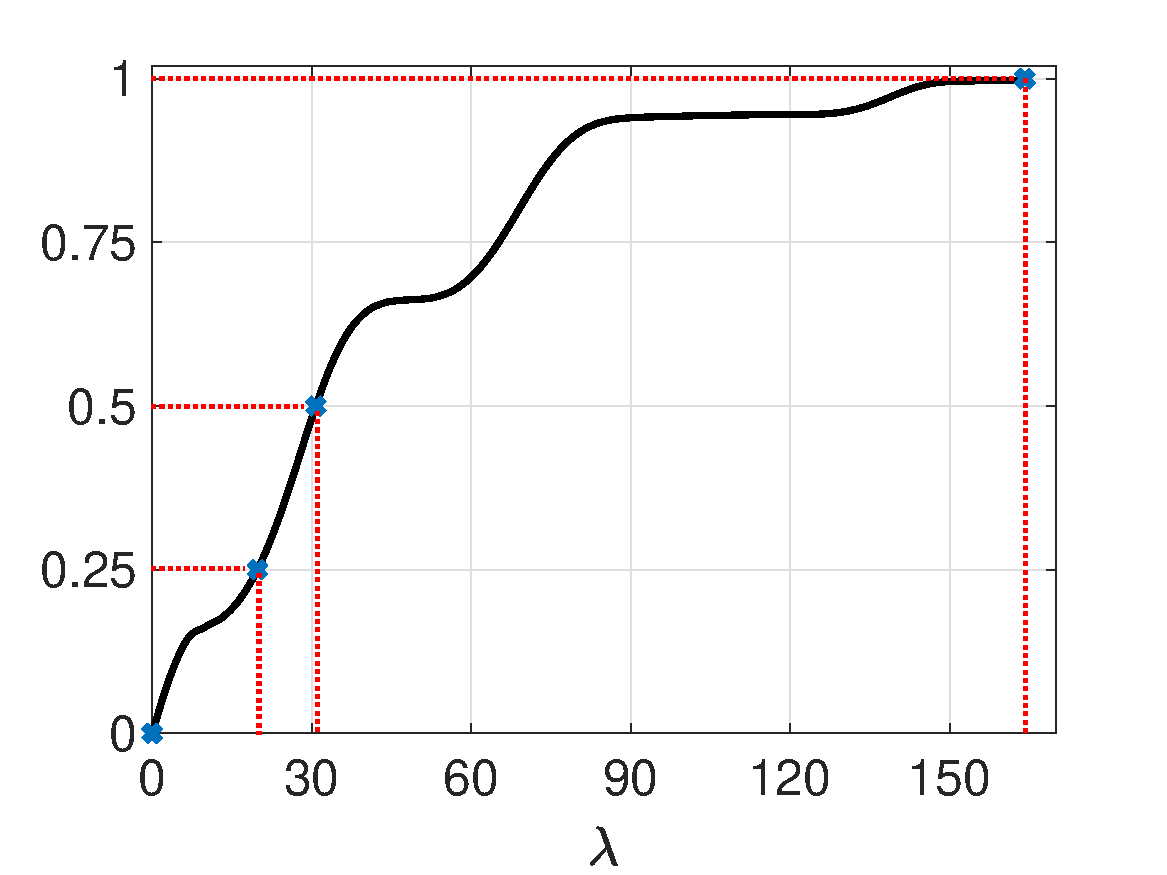
\includegraphics[width=1.1\linewidth]{fig_cdf}}
\centerline{~~\small{(a)}}
\end{minipage}
\begin{minipage}[m]{0.49\linewidth}
\centerline{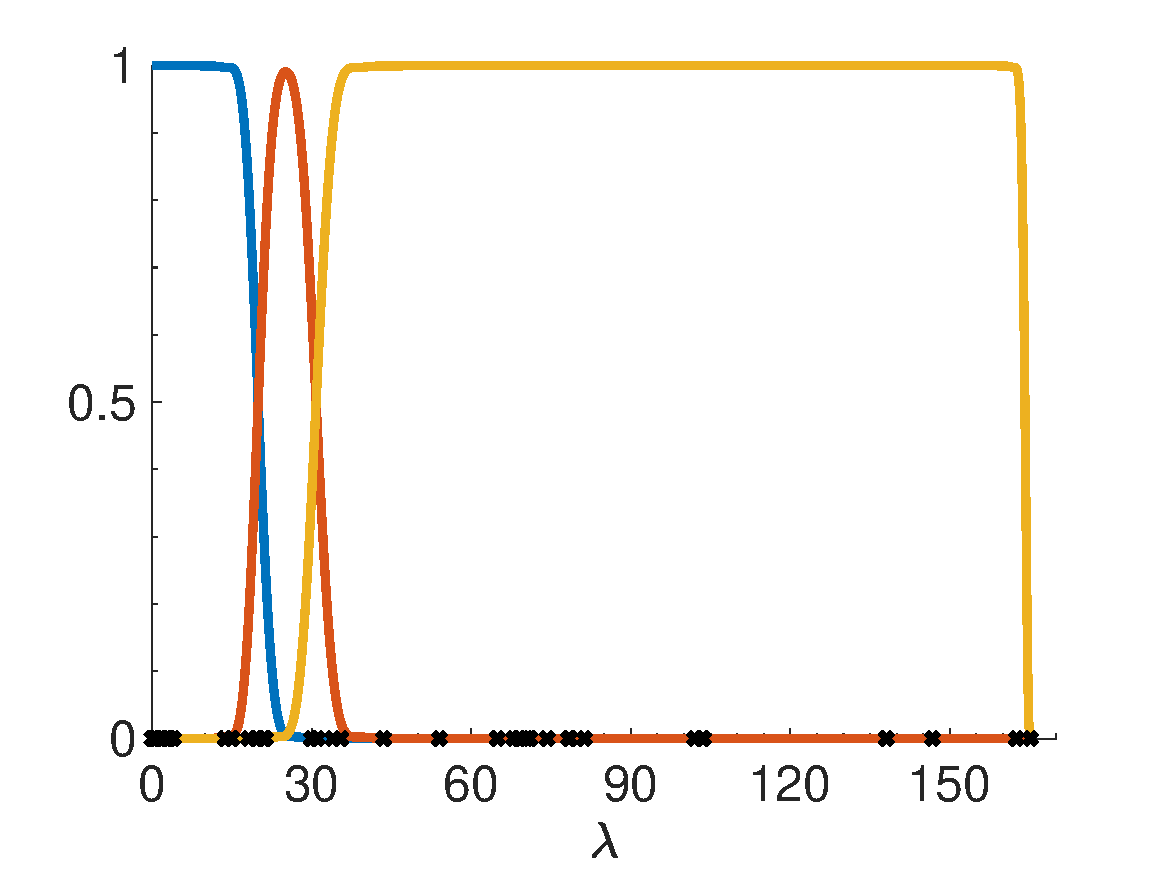
\includegraphics[width=1.1\linewidth]{fig_orig_fb}}
\centerline{~~\small{(b)}}
\end{minipage} \\
\begin{minipage}[m]{0.49\linewidth}
\centerline{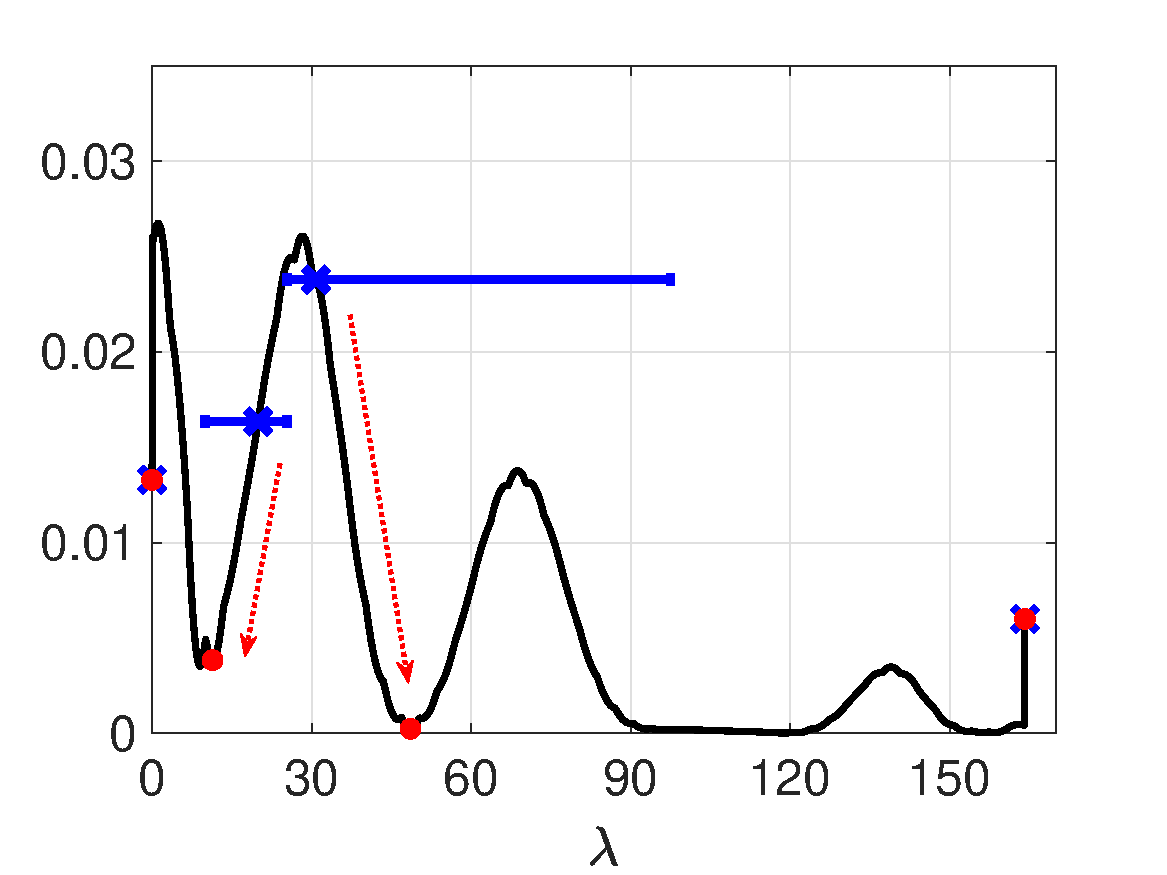
\includegraphics[width=1.1\linewidth]{fig_pdf}}
\centerline{~~\small{(c)}}
\end{minipage}
\begin{minipage}[m]{0.49\linewidth}
\centerline{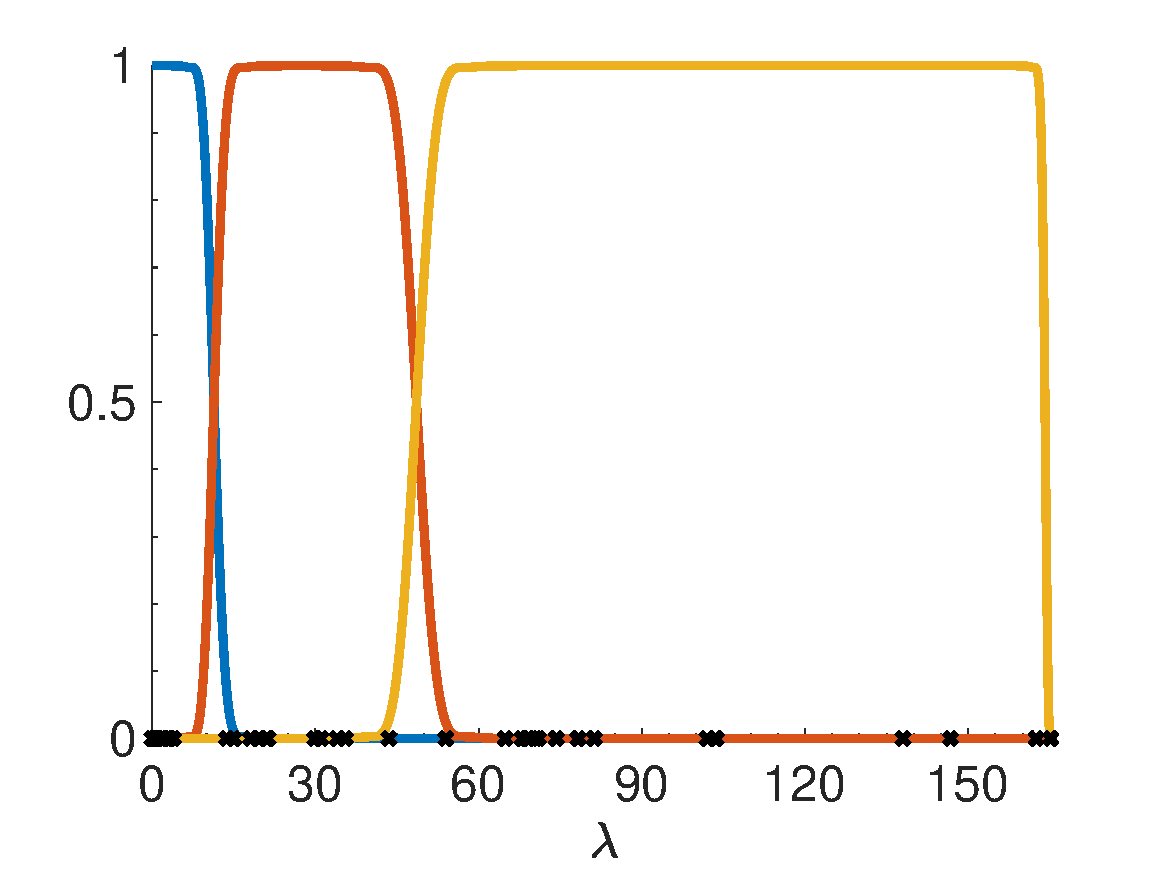
\includegraphics[width=1.1\linewidth]{fig_updated_fb}}
\centerline{~~\small{(d)}}
\end{minipage}
\caption{{(a) The approximate cumulative spectral density function, $\tilde{P}_{\lambda}(\cdot),$ for the net25 graph described in Figure \ref{Fig:approx_filtering_error}. The blue X marks correspond to the initial choice of band endpoints computed by taking the inverse of logarithmically spaced points on the vertical axis. (b) The degree 80 Jackson-Chebyshev approximations to the ideal filters defined by the initial choice of band ends from (a). (c) The objective function of \eqref{Eq:adjustment} (a discrete approximation of the spectral density function $p_{\lambda}(\cdot)$) with $\Delta=.001$. The blue horizontal lines correspond to the search intervals ${\cal I}_1$ and ${\cal I}_2$, and the red circles represent the adjusted band ends $\{\tau_m\}_{m=0,1,2,3}$. (d) The degree 80 Jackson-Chebyshev approximations to the ideal filters defined by the adjusted choice of band ends. Note that the errors between the approximate filters and ideal bandpass filters are concentrated in regions with fewer eigenvalues (gaps in the spectrum).}}\label{Fig:fb_design}
\end{figure}

\subsubsection{Adjusting the band ends} \label{Se:adjust}

In order to make the filters more amenable to approximation, we then adjust the initial choice of band endpoints so that they lie in lower density regions of the spectrum. Specifically, for each $m=1,2,\ldots,M-1$ and some choice of $\Delta>0$, we let the final endpoint be
\begin{align} \label{Eq:adjustment}
\tau_m^* = \argmin_{\tau \in {\cal I}_m} \left\{\frac{\tilde{P}_{\lambda}(\tau+\Delta)-\tilde{P}_{\lambda}(\tau-\Delta)}{2\Delta}\right\},
\end{align}
%search for the minimizer of $\frac{\tilde{P}_{\lambda}(\cdot)}{2 \Delta}$ 
where ${\cal I}_m$ is an interval around the initial choice of $\tau_m$. Figure \ref{Fig:fb_design}(c) shows the objective function in \eqref{Eq:adjustment}, along with the initial band ends, search intervals, and adjusted band ends. Comparing Figure \ref{Fig:fb_design}(b) and Figure \ref{Fig:fb_design}(d), we 
see that adjusting the band ends leads to fewer eigenvalues falling close to the borders of the filters, reducing the error incurred by the polynomial approximation process.
 





%\begin{itemize}
%\item refer back to error equation, Design to aim for spectral gaps, more amenable to polynomial approximation
%\item Don't know where these gaps are, but can estimate the spectral distribution
%\item References, and KPM, approximation of the eigenvalue distribution based on the spectrum slicing method of \cite[Section 3.3]{parlett}
%\item Set the initial band ends either logarithmically or evenly spaced, spectrum-adapted or not, similar to the tight warped filter bank design of \cite{shuman2013spectrum}.
%\item Then search for local minima in the pdf 
%\end{itemize}
%One possibility for efficiently designing the filter bank without full knowledge of the spectrum is to use . These can either be adapted to the width of the spectrum using only an estimate of the maximum eigenvalue, or to an . In either case, the filters can then be applied using t. %However, the interpolation step needs to be adjusted accordingly. 

%Issues that arise in this context include designing the filter bank to be , 




\section{Non-Uniform Random Sampling and Reconstruction}
Both the partitioning of the vertices into uniqueness sets described in Algorithm 1 and the synthesis via interpolation in \eqref{Eq:synth} require a full eigendecomposition of the graph Laplacian to compute the matrix ${\bf U}$. In this section, we examine more efficient sampling and reconstruction methods that do not require the full eigendecomposition.


\subsection{Sampling distribution}
Two broad approaches to more efficient sampling have recently been investigated: greedy methods \cite{chen2015discrete,anis2014towards,tsitsvero2016uncertainty,anis2016efficient} and random sampling methods \cite{shomorony,PuyTGV15,chen2016signal}. Reference \cite{anis2016efficient} has a nice review of the computational complexities of the various greedy routines for identifying uniqueness sets. Most of these are designed specifically for lowpass signals. 
 
We adapt the non-uniform random sampling method of \cite{PuyTGV15}, which scales more efficiently than greedy methods. Namely, for the $m^{th}$ band, we identify the downsampling set $\V_m$ by sampling the vertices $\V$ {\color{red} without replacement} according to a discrete probability distribution ${\boldsymbol \omega}_m$. To minimize the graph weighted coherence, it is ideal to take ${\boldsymbol \omega}_m(i) \propto ||{\bf U}_{{\cal R}_m}^{\top} {\boldsymbol \delta}_i ||_2^2$ \cite{PuyTGV15}; however, we do not have access to ${\bf U}_{{\cal R}_m}$. Instead, we take 
\begin{align}\label{Eq:samp_dist}
{\boldsymbol \omega}_m(i) \propto ||(\tilde{h}_m(\L){\bf X})^{\top} {\boldsymbol \delta}_i ||_2^2,
\end{align}
which \cite{PuyTGV15} shows is an unbiased estimator of $||{\bf U}_{{\cal R}_m}^{\top} {\boldsymbol \delta}_i ||_2^2$ when ${\bf X}$ is the random matrix from \eqref{Eq:hutch4}. Since we already compute and store the series of matrices $\bar{T}_k(\L){\bf X}$ for the spectral density estimation of Section \ref{Se:spectral_density}, we just need to compute the polynomial approximation coefficients $\{\alpha_k\}$ in \eqref{Eq:hutch4} for $h_m(\lambda)$ in order to compute $\tilde{h}_m(\L){\bf X}$.

%\begin{itemize}
%%\item Fast sampling and reconstruction. Two main approaches to sampling: greedy and random
%%\item Most work on lowpass/smooth signals
%%\item Estimating number of measurements for each band
%\item Review of non-uniform random sampling literature
%%\item Reconstruction - emphasize change from only lowpass bands
%%\item {\color{red} Solving the reconstruction equation efficiently and robustly}
%\end{itemize}

% The random sampling method proposed in \cite{PuyTGV15} does not require the full eigendecomposition of the graph Laplacian and therefore scales significantly better with the size of the graph.
%We are currently examining whether there is a way to extend the approach of \cite{PuyTGV15} to non-uniformly randomly sample in a manner that leads with high probability to uniqueness sets for higher bands of the graph Laplacian spectrum. 


{\color{red}
\begin{itemize}
\item Add intuition about which nodes receive high weights and diagram of the matrix to support that. Then refer to figures.
\item Check that embedding theorem works for upper bands as well and mention
\item Note that the benefits of non-uniform sampling come when eigenvectors are more localized (c.f., Section 5.1.2 of Gilles' paper); this is especially important for high pass filters
\item Link to literature on column subset selection (statistical leverage)
\item Note that for any walk regular graph, optimal sampling distribution is uniform; give some examples (cycle, path, grid, vertex transitive graphs, etc.); cite godsil paper on symmetry and eigenvectors
\end{itemize}
}

\subsection{Number of samples}

To yield a critically sampled transform, one option is to choose the number of samples for each band to be in correspondence with the initial filter bank design. For example, if the filter bank is designed to be adapted to the spectrum with logarithmic spacing, we can choose $\frac{N}{2}$ samples for the highest band, $\frac{N}{4}$ for the next highest, and so forth. However, the adjustments we make in Section \ref{Se:adjust} affect the number of eigenvalues contained in each band. Since we have an estimate of the cumulative spectral distribution, one approximation for the number of samples in the adjusted $m^{th}$ band is to round $N \cdot (\tilde{P}_{\lambda}(\tau_{m})-\tilde{P}_{\lambda}(\tau_{m-1}))$. As a band end $\tau_m$ may fall at a point where $\tilde{P}_\lambda$ has been interpolated via cubic functions, another option is to estimate the number of eigenvalues between $\tau_{m-1}$ and $\tau_m$, once again with the stochastic trace estimator in \eqref{Eq:hutch3}, except using the bandpass filter $h_m(\lambda)$ from \eqref{Eq:bandpass}. We already compute $\tilde{h}_m(\L){\bf X}$ to calculate the sampling distribution in \eqref{Eq:samp_dist}. We can substitute the columns $\tilde{h}_m(\L){\bf x}^{(j)}$ of this matrix into 
%Since we have already computed and stored the series of matrices $\bar{T}_k(\L){\bf X}$, we just need to compute the polynomial approximation coefficients $\{\alpha_k\}$ in \eqref{Eq:hutch4} for  $h_m(\lambda)$, and substitute the resulting $\tilde{h}_m(\L){\bf x}^{(j)}$ values into 
\eqref{Eq:hutch3} for an estimate of the number of eigenvalues in the $m^{th}$ band. An added benefit of this extra step is that the thresholds $\{\tau_m\}$ are chosen to be in areas of low spectral density, which improves the accuracy of the eigenvalue count estimate \cite{di2016efficient}. If critical sampling is desired, we can make small adjustments to ensure the total number of samples is equal to $N$. Our default is to add samples to the lowest band if the estimated total is lower than $N$, and remove samples from the highest band if the estimated total is higher than $N$.

Note that due to the polynomial approximation, the dimension of $\hbox{col}(\tilde{h}_m(\L))$ is at least as large as the dimension of $\hbox{col}({h}_m(\L))$, with the difference depending on the number of Laplacian eigenvalues just outside the end points of $h_m(\cdot)$ and the degree of approximation used for $\tilde{h}_m(\cdot)$. Therefore, we expect that to perfectly reconstruct signals in $\hbox{col}(\tilde{h}_m(\L))$, we need more samples than the number of eigenvalues in the support of $h_m(\cdot)$. In Section \ref{Se:ill2}, we explore how the reconstruction error is reduced as we increase the number of samples in each band. The tradeoff is the loss of critical sampling, as the total number of samples extends beyond $N$. 


%{\color{red} In practice, these two methods of estimating the number of eigenvalues in each band do not }

%\begin{itemize}
%\item Would expect critical sampling won't work with approximate filtering, because actual support of each projection is wider
%\item Review number of samples guarantee from \cite{PuyTGV15} with high probability; how does this scale across channels
%%\item $\tilde{P}_{\lambda}(\tau_{m})-\tilde{P}_{\lambda}(\tau{m-1})$
%%\item However, since we have also computed and stored the series of matrices $\bar{T}_k(\L){\bf X}$ in XXX, we can estimate the number of samples in each band by 
%\item With either of these, we can make a small adjustment to ensure the filter bank is critically sampled
%%\item Or just use design numbers (e.g., logarithmically spaced). put first, doesn't account for adjustments
%%\item In practice
%%\item 
%\end{itemize}
\subsection{Interpolation}
The exact interpolation \eqref{Eq:synth} requires the eigenvector matrix ${\bf U}$, and in case $U_{\V_m,{\cal R}_m}$ is not full rank, the standard least squares reconstruction for the $m^{th}$ channel
\begin{align}
{\bf f}_{m,{rec}}=\mathbf{U}_{{\cal R}_m}(\mathbf{U}_{\V_m,{\cal R}_m}^{\top}\mathbf{U}_{\V_m,{\cal R}_m})^{-1}\mathbf{U}_{\V_m,{\cal R}_m}^{\top}{\bf y}_{\V_m}
\end{align}
also requires ${\bf U}_{{\cal R}_m}$. One option explored in \cite{halko,paratte} is to leverage $\{\bar{T}_k(\L){\bf X}\}$ again to approximate the column space of ${\bf U}_{{\cal R}_m}$ by filtering at least $|{\cal R}_m|$ standard normal random vectors with the filter $\tilde{h}_m(\cdot)$, possibly followed by orthonormalization via QR factorization.

A second approach suggested in \cite{PuyTGV15} to efficiently reconstruct lowpass signals is to relax the optimization problem
\begin{align*}
\min_{{\bf z} \in \hbox{col}({\bf U}_{{\cal R}_m})} ||{\boldsymbol \Omega}_{m,\V_m}^{-\frac{1}{2}}\left({\bf M_m z}-{{\bf y}_{\V_m}} \right) ||_2
\end{align*} 
to 
\begin{align}\label{Eq:approx_rec_opt}
\min_{{\bf z} \in \R^N} ||{\boldsymbol \Omega}_{m,\V_m}^{-\frac{1}{2}}\left({\bf M_m z}-{{\bf y}_{\V_m}} \right) ||_2+{\bf z}^{\top}\varphi_m(\L){\bf z},
\end{align} 
where ${\boldsymbol \Omega}_{m,\V_m}$ is a $|\V_m| \times |\V_m|$  diagonal matrix with the $m^{th}$ channel sampling weights of $\V_m$ along the diagonal. The regularization term ${\bf z}^{\top}\varphi_m(\L){\bf z}$ in \eqref{Eq:approx_rec_opt} penalizes reconstructions with support outside of the desired spectral band. For lowpass signals, Puy et al. \cite{PuyTGV15} take the penalty function $\varphi_m(\lambda)$ to be a nonnegative, nondecreasing polynomial, such as $\kappa \lambda^l$, with $\kappa>0$ and $l$ a positive integer. For more general classes of signals (i.e., the midpass and highpass signals output from the higher bands of the proposed filter bank), it is important to keep the nonnegativity property, in order to ensure that $\varphi_m(\L)$ is positive semi-definite and the optimization problem \eqref{Eq:approx_rec_opt} is convex. However, we can drop the nondecreasing requirement, and instead choose penalty functions concentrated outside the $m^{th}$ spectral band. Options we explore include (i) $\varphi_m(\lambda)=\kappa\left[1-\tilde{h}(\lambda)\right]$; (ii) $\varphi_m(\lambda)=\frac{1}{\tilde{h}(\lambda)+\epsilon}-\frac{1}{1+\epsilon}$ {\color{red} Check nonnegativity}; and (iii) {\color{red} Spline approach of Saad. See Figure \ref{Fig:penalty} for example graphs of these penalty functions.}

\begin{figure}[tb]
\begin{minipage}[m]{0.49\linewidth}
\centerline{\small{$K=20$}}
\centerline{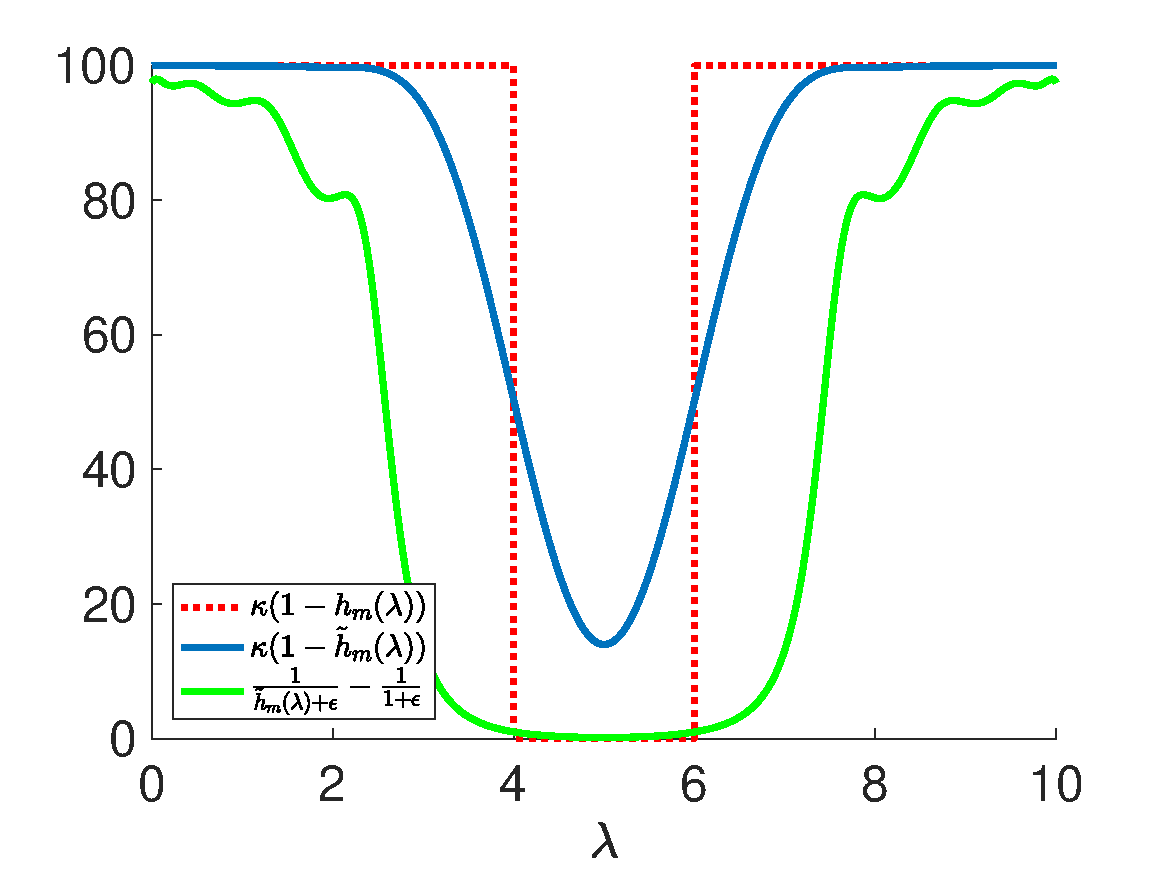
\includegraphics[width=1.1\linewidth]{fig_reg_filters_20}}
\centerline{~~\small{(a)}}
\end{minipage}
\begin{minipage}[m]{0.49\linewidth}
\centerline{\small{$K=50$}}
\centerline{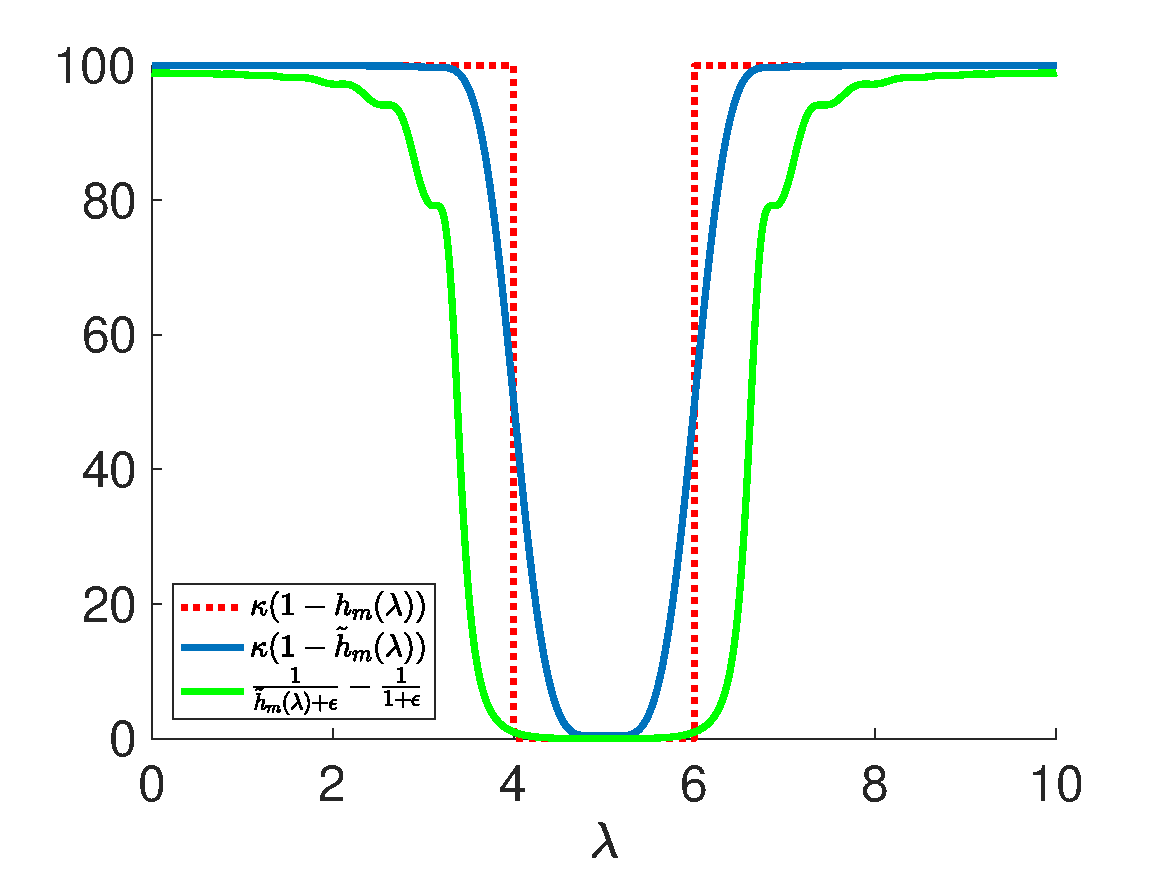
\includegraphics[width=1.1\linewidth]{fig_reg_filters_50}}
\centerline{~~\small{(b)}}
\end{minipage} 
\caption{Example penalty filters $\varphi_m$ for the regularization term in \eqref{Eq:approx_rec_opt}, with $\epsilon=\frac{1}{\kappa}=0.01$. Here, $\tilde{h}_m$ is a Jackson-Chebyshev polynomial approximation of $h_m$ of degree 20 and 50 in (a) and (b), respectively.}\label{Fig:penalty}
\end{figure}

From the first-order optimality conditions, the solution to \eqref{Eq:approx_rec_opt} is the solution to the linear system of equations
\begin{align}\label{Eq:approx_rec_sol}
\Bigl(M_m^{\top}{\boldsymbol \Omega}_{m,\V_m}^{-1}M_m+\varphi_m(\L)\Bigr){\bf  z}=M_m^{\top}{\boldsymbol \Omega}_{m,\V_m}^{-1}{\bf y}_{\V_m},
\end{align}
which can be solved, for example, with the preconditioned conjugate gradient method. {\color{red}Add more details? Preconditioner? How to compute $\varphi_m(\L){\bf z}$.}

%\begin{itemize}
%%\item standard with U
%%\item one option is to leverage $\{\bar{T}_k(\L){\bf X}\}$ again to approximate the column space
%%\item Another is to follow Gilles' approach (optimization problem, relaxation)
%\item Solution
%%\item They take nonnegative and nondecreasing for lowpass priors. The nonnegative is important to keep the problem convex, but we can use any penalty function that 
%%\item Example penalty functions: $1-\tilde{h}(\lambda)$, $\frac{1}{h(\lambda)+\epsilon}-\frac{1}{1+\epsilon}$, spline based approach of Saad. 
%\item how to solve the solution
%%Compare these empirically in the next section.
%\end{itemize}

%If $y_{\V_m}$ are the analysis coefficients of the $m^{th}$ branch, the standard least squares reconstruction is to solve $x_m^*=\argmin_{x \in \R^{k_m}} ||\mathbf{U}_{{\cal R}_m}x - y_{\V_m} ||_2$, and let $f_{m,{rec}}(\V_m)=y_{\V_m}$ and $f_{m,{rec}}(\V_m^c)=\mathbf{U}_{\V_m^c,{\cal R}_m}x_m^*$; however, this requires a full eigendcomposition of $\L$ to get $\mathbf{U}$. Our ongoing work includes developing an efficient optimization algorithm that directly uses a function of $\L$ rather than $\mathbf{U}$ to stably reconstruct signals supported on a specific spectral band from its samples. 


{\color{red}
[Say something about which option we choose and why, and point to empirical comparison in the next section.]
The analysis and synthesis operations for the proposed scalable $M$-channel filter bank are summarized in Algorithms XXX and ZZZ, respectively.

\begin{itemize}
\item Theoretical analysis of reconstruction error
\item Reconstruction robustness to noisy or thresholded filter bank coefficients (see, e.g., \cite[Section III.B]{anis2016efficient} for more on reconstruction stability)
\end{itemize}
}
%\subsection{Reconstruction robustness to noisy or thresholded filter bank coefficients} \label{Se:noisy_ext}
%For any partition into uniqueness sets, the proposed transform perfectly recovers the signal from the analysis coefficients. However, the choice of the downsampling patterns and interpolation method can dramatically affect the stability of the reconstruction if the analysis coefficients are corrupted by noise or are only partially available, or approximate filters are used to speed up the transform . Thus, we plan to investigate the role of the initial choice of the $\gamma_i$'s in Algorithm \ref{Al:uniqueness} in improving the stability of the reconstruction.
{\color{red}
\section{Properties of the Fast M-CSFB Transform}
\subsection{Joint vertex-frequency localization of the atoms}
\subsection{Computational complexity}
}
{\color{blue}
\section{Illustrative Examples II: Approximate Calculations} \label{Se:ill2}
\begin{itemize}
\item Reconstruction of bandpass signal. Tradeoff between number of samples and reconstruction error. Show different methods? 
\item Repeat bunny compression example. Much worse?
\item Make sure to have some very large examples and show computation times
\end{itemize}
}


\section{Conclusion and Extensions}
\label{Sec:ongoing}
{\color{red} %Eliminate once we've covered all of these issues elsewhere.}

Insert key findings here
\begin{itemize}
\item Leveraged the computation of $\{\bar{T}_k(\L){\bf X}\}$ in multiple ways 
\item Can be seen as a coarse, fast GFT, maybe compare to that literature
\end{itemize}
}

%\subsection{Iterated filter bank} 
As with the classical wavelet construction, it is possible to iterate the filter bank on the output from the lowpass channel.
This could be beneficial, for example, in the case that we want to visualize the graph signal at different resolutions on  a sequence of coarser and coarser graphs. An interesting question for future work is how iterating the filter bank with fewer channels at each step compares to a single filter bank with more channels and each filter supported on a smaller region of the spectrum.


\balance
\bibliographystyle{IEEEtran}
{\small \bibliography{mcsfb_refs}}


\end{document}
